\documentclass[11pt,a4paper]{article}

\usepackage[utf8]{inputenc}
\usepackage[T1]{fontenc}
\usepackage[spanish,es-nodecimaldot]{babel}
\usepackage{lmodern}
\usepackage{microtype}
\usepackage[margin=2.05cm,headheight=16pt]{geometry}
\usepackage{amsmath,amssymb,mathtools}
\usepackage{graphicx}
\usepackage{booktabs,tabularx,longtable,array}
\usepackage{enumitem}
\usepackage{xcolor}
\usepackage{float}
\usepackage{caption}
\usepackage{subcaption}
\usepackage[most]{tcolorbox}
\usepackage{titlesec}
\usepackage{fancyhdr}
\usepackage{xurl}
\usepackage{hyperref}

\graphicspath{{../doc_figures/}}

\definecolor{Navy}{HTML}{12355B}
\definecolor{Blue}{HTML}{1C6E8C}
\definecolor{Teal}{HTML}{0F8B8D}
\definecolor{Gold}{HTML}{D99B2B}
\definecolor{Ink}{HTML}{25313C}
\definecolor{SoftBlue}{HTML}{EDF6FA}
\definecolor{SoftGold}{HTML}{FFF7E6}
\definecolor{SoftGray}{HTML}{F3F5F7}
\definecolor{SoftRed}{HTML}{FFF0EF}
\definecolor{Red}{HTML}{A33A32}
\definecolor{Green}{HTML}{287A55}

\hypersetup{
  colorlinks=true,
  linkcolor=Navy,
  citecolor=Teal,
  urlcolor=Blue,
  pdftitle={Manual teorico pedagogico de sistemas dinamicos y caos},
  pdfauthor={Toolbox Chaos}
}
\urlstyle{same}

\setlength{\parindent}{0pt}
\setlength{\parskip}{0.45em}
\setlist[itemize]{leftmargin=1.35em,itemsep=0.18em,topsep=0.25em}
\setlist[enumerate]{leftmargin=1.6em,itemsep=0.22em,topsep=0.25em}
\renewcommand{\arraystretch}{1.18}

\titleformat{\section}
  {\Large\sffamily\bfseries\color{Navy}}
  {\thesection}{0.65em}{}
\titleformat{\subsection}
  {\large\sffamily\bfseries\color{Blue}}
  {\thesubsection}{0.55em}{}
\titleformat{\subsubsection}
  {\normalsize\sffamily\bfseries\color{Teal}}
  {}{0pt}{}

\pagestyle{fancy}
\fancyhf{}
\fancyhead[L]{\sffamily\small Toolbox Chaos}
\fancyhead[R]{\sffamily\small Manual teórico pedagógico}
\fancyfoot[L]{\sffamily\scriptsize Sistemas dinámicos y análisis numérico}
\fancyfoot[R]{\sffamily\small \thepage}
\renewcommand{\headrulewidth}{0.4pt}

\newcommand{\R}{\mathbb{R}}
\newcommand{\dist}{\operatorname{dist}}
\newcommand{\code}[1]{\texttt{#1}}
\newcommand{\gui}[1]{\textsf{\emph{#1}}}
\newcommand{\term}[1]{\textcolor{Navy}{\emph{#1}}}
\newcommand{\dd}{\,\mathrm{d}}

\newtcolorbox{objectivebox}{
  enhanced,breakable,colback=SoftBlue,colframe=Blue,
  boxrule=0.75pt,arc=1.5mm,left=2mm,right=2mm,top=1.5mm,bottom=1.5mm,
  title={Objetivo de aprendizaje},fonttitle=\sffamily\bfseries
}
\newtcolorbox{activitybox}[1]{
  enhanced,breakable,colback=SoftGold,colframe=Gold,
  boxrule=0.75pt,arc=1.5mm,left=2mm,right=2mm,top=1.5mm,bottom=1.5mm,
  title={#1},fonttitle=\sffamily\bfseries
}
\newtcolorbox{evidencebox}[1]{
  enhanced,breakable,colback=SoftGray,colframe=Navy,
  boxrule=0.7pt,arc=1.5mm,left=2mm,right=2mm,top=1.5mm,bottom=1.5mm,
  title={#1},fonttitle=\sffamily\bfseries
}
\newtcolorbox{warningbox}{
  enhanced,breakable,colback=SoftRed,colframe=Red,
  boxrule=0.7pt,arc=1.5mm,left=2mm,right=2mm,top=1.5mm,bottom=1.5mm,
  title={Límite de interpretación},fonttitle=\sffamily\bfseries
}
\newcommand{\didactic}[1]{%
  \par\medskip\noindent{\sffamily\itshape\color{Teal}#1.}\enspace}
\newcommand{\lecturaseccion}[1]{%
  \par\noindent{\sffamily\scriptsize\color{Teal}Lectura complementaria}\footnote{%
  \textbf{Lectura complementaria.} #1}\par}

\begin{document}

\pagenumbering{roman}
\begin{titlepage}
\pagecolor{SoftBlue}
\color{Ink}
\vspace*{1.2cm}
{\sffamily\Large\color{Blue} Toolbox Chaos}\par
\vspace{0.55cm}
{\sffamily\bfseries\fontsize{28}{33}\selectfont
Manual teórico pedagógico\par}
\vspace{0.35cm}
{\sffamily\fontsize{17}{22}\selectfont
  Sistemas dinámicos, caos e interpretación responsable de resultados\\
  numéricos\par}
\vspace{0.9cm}
\begin{tcolorbox}[colback=white,colframe=Teal,boxrule=1pt,arc=2mm]
Este manual desarrolla los conceptos matemáticos que permiten leer las gráficas de
Toolbox Chaos. Cada unidad parte de una
intuición, formula el concepto, lo conecta con una pestaña de la interfaz y termina
con una actividad de contraste. La meta es construir evidencia mediante cálculos,
gráficas y criterios de interpretación.
\end{tcolorbox}
\vfill
{\sffamily\large Contenido temático}\par
\vspace{0.3cm}
\begin{tabularx}{\textwidth}{>{\sffamily\bfseries\color{Navy}}p{0.25\textwidth}X}
Fundamentos & Estado, modelado, flujos de una y dos dimensiones, estabilidad, oscilaciones e integración numérica.\\
Caos y diagnósticos & Mapas, bifurcaciones, cuencas, Lyapunov, espectros, recurrencia y dimensión.\\
Sistemas y aplicaciones & Lorenz, Rössler, Chua, Duffing--Ueda, retardo, alta dimensión y orden fraccionario.\\
Curso y proyecto & Secuencia de 16 unidades, laboratorios reproducibles, actividades y proyecto integrador.\\
\end{tabularx}
\vfill
{\small\sffamily Edición pedagógica independiente. Las figuras son productos del
propio software o esquemas elaborados para este manual; las figuras de los libros
citados permanecen en sus fuentes originales.}
\end{titlepage}
\nopagecolor
\pagenumbering{arabic}

\tableofcontents
\vfill
\begin{evidencebox}{Tres rutas de lectura}
\textbf{Ruta conceptual:} unidades 1--7 para construir el lenguaje geométrico y
algebraico. \textbf{Ruta computacional:} unidades 8--14 para integrar, diagnosticar
y contrastar datos. \textbf{Ruta de investigación:} unidades 15--16, proyecto final,
banco de problemas y guía de comunicación. En cualquiera de las rutas conviene leer
primero la pregunta de interpretación y cerrar cada práctica con su control numérico.
\end{evidencebox}
\newpage

\section*{Uso del manual teórico}
\addcontentsline{toc}{section}{Organización y criterios de estudio}

La teoría de sistemas dinámicos combina tres lenguajes: ecuaciones, geometría y
datos numéricos. Conviene pasar continuamente de uno a otro. Strogatz propone
construir primero intuición geométrica y después formalizarla; Devaney muestra que
las propiedades globales requieren hipótesis precisas; Sprott explota el cálculo y la
visualización como laboratorio para descubrir patrones \cite{strogatz2024,devaney1989,sprott1993}.
Aquí se integran esas tres miradas.

% Plan curricular. Se incluye desde manual_teorico_pedagogico.tex.

\subsection*{Programa de sistemas dinámicos y caos}
\phantomsection
\addcontentsline{toc}{subsection}{Plan de curso: de los modelos a la evidencia dinámica}

\begin{objectivebox}
Al concluir esta ruta de dieciséis unidades, la persona estudiante podrá formular y
adimensionalizar modelos, analizar equilibrios y bifurcaciones, distinguir flujos de
mapas, interpretar retratos, series y diagramas, y construir diagnósticos de caos con
controles numéricos explícitos. El producto final será un expediente reproducible que
conecte ecuaciones, algoritmos, gráficas y límites
de la evidencia.
\end{objectivebox}

\paragraph{Duración, modalidad y perfil de ingreso.}
El curso está diseñado para licenciatura avanzada, ingeniería o primer posgrado. Se
propone una duración de dieciséis semanas, con dos horas de teoría, una de discusión y
dos de laboratorio por semana. Puede impartirse en catorce semanas fusionando las
unidades 1--2 y 14--15. Cada práctica conserva sistema, parámetros, condición inicial,
integrador, paso, horizonte, transitorio y versión del software.

\paragraph{Prerrequisitos verificables.}
El curso comienza con una introducción al caos. Se requieren cálculo diferencial e integral,
álgebra lineal elemental, números complejos y lectura de ecuaciones diferenciales de
primer orden. Antes de iniciar se debe poder: calcular traza, determinante y
autovalores de una matriz \(2\times2\); derivar un polinomio; distinguir unidades de
valores numéricos; representar \(y=f(x)\); y reconocer sus intersecciones con \(y=x\).

\begin{activitybox}{Diagnóstico de entrada}
Para \(A=\left(\begin{smallmatrix}0&1\\-2&-3\end{smallmatrix}\right)\), calcule
\(\operatorname{tr}A\), \(\det A\) y los autovalores. Para
\(\dot x=x(1-x)\), encuentre los equilibrios y determine el signo de \(\dot x\) en
los intervalos que separan. Finalmente explique por qué \(x(t)\) contra \(t\) y
\(y\) contra \(x\) responden preguntas distintas. El diagnóstico asigna lecturas de
nivelación y se mantiene separado de la calificación.
\end{activitybox}

\lecturaseccion{Nivelación: Morris W. Hirsch, Stephen Smale y Robert L. Devaney,
\emph{Differential Equations, Dynamical Systems, and an Introduction to Chaos},
3.\textsuperscript{a} ed., capítulo 1, ``First-Order Equations'', y capítulos 2--4,
``Planar Linear Systems'', ``Phase Portraits for Planar Systems'' y
``Classification of Planar Systems''; Steven H. Strogatz, \emph{Nonlinear Dynamics
and Chaos with Applications to Physics, Biology, Chemistry, and Engineering},
2.\textsuperscript{a} ed., secciones 2.1, ``A Geometric Way of Thinking'', y 5.1,
``Definitions and Examples''.}

\paragraph{Competencias evaluables.}
\begin{description}
  \item[RA1.] Traducir una situación a variables, parámetros, ecuaciones y escalas
  adimensionales, declarando las hipótesis del modelo.
  \item[RA2.] Analizar flujos unidimensionales con líneas de fase, estabilidad,
  potenciales y formas normales.
  \item[RA3.] Clasificar sistemas lineales planos y usar el Jacobiano para formular
  predicciones locales en sistemas no lineales.
  \item[RA4.] Construir nullclines, retratos y mapas de retorno, y aplicar criterios
  de existencia o exclusión de ciclos.
  \item[RA5.] Reconocer bifurcaciones y rutas al caos, distinguiendo un barrido
  numérico con una demostración.
  \item[RA6.] Analizar mapas mediante iteración, telarañas, multiplicadores y
  dinámica simbólica.
  \item[RA7.] Comparar Lorenz, Rössler, Chua y Duffing--Ueda desde ecuaciones,
  disipación, simetrías, series y proyecciones.
  \item[RA8.] Interpretar Lyapunov, FFT/PSD y dimensiones con estudios de
  convergencia y sensibilidad.
  \item[RA9.] Delimitar modelos con retardo, alta dimensión, dinámica conservativa,
  caos transitorio, sincronización, control y memoria fraccionaria.
  \item[RA10.] Comunicar un experimento con datos suficientes para repetirlo y
  auditar sus afirmaciones.
\end{description}

\paragraph{Evaluación.}
\begin{longtable}{>{\raggedright\arraybackslash}p{0.29\linewidth}
                  >{\centering\arraybackslash}p{0.11\linewidth}
                  >{\raggedright\arraybackslash}p{0.50\linewidth}}
\toprule
Producto & Peso & Evidencia mínima \\
\midrule
\endhead
Problemas analíticos & \(15\%\) & Derivación, hipótesis, unidades y clasificación.\\
Ocho bitácoras de laboratorio & \(25\%\) & Contrato numérico, datos, figura,
interpretación y contraste.\\
Dos estudios de caso & \(20\%\) & Un mapa y un flujo, cada uno con tres vistas y un
indicador cuantitativo.\\
Examen conceptual y algebraico & \(15\%\) & Definiciones operativas, cálculos locales
y lectura crítica de gráficas.\\
Proyecto integrador & \(25\%\) & Pregunta, protocolo, reproducción cruzada, datos,
discusión de incertidumbre y defensa.\\
\bottomrule
\end{longtable}

\begin{evidencebox}{Regla transversal de suficiencia}
Una captura aislada sólo demuestra que se produjo una imagen. Una conclusión dinámica
requiere el sistema identificado, el contrato numérico, al menos un contraste
pertinente y una interpretación compatible con el algoritmo. En todo el curso se
separan observación, diagnóstico numérico y afirmación matemática.
\end{evidencebox}

\paragraph{Secuencia de las dieciséis unidades.}
{\small
\setlength{\tabcolsep}{4pt}
\begin{longtable}{>{\centering\arraybackslash}p{0.045\linewidth}
                  >{\raggedright\arraybackslash}p{0.23\linewidth}
                  >{\raggedright\arraybackslash}p{0.30\linewidth}
                  >{\raggedright\arraybackslash}p{0.27\linewidth}}
\toprule
U & Núcleo & Resultado observable & Laboratorio \\
\midrule
\endhead
1 & Estado, órbita, flujo y mapa & Distingue tiempo, iteración y proyección &
Lorenz en tres vistas coordinadas.\\
2 & Modelado y escalamiento & Obtiene grupos adimensionales & Duffing en
\gui{Crear sistema}.\\
3 & Flujos 1D y formas normales & Construye líneas de fase &
\(\dot x=\mu-x^2\) y \(\dot x=\mu x-x^3\).\\
4 & Sistemas lineales 2D & Usa el plano traza--determinante & Nodo, silla, centro y
foco.\\
5 & Jacobiano y nullclines & Conecta geometría global y predicción local &
Modelo de interacción de dos poblaciones.\\
6 & Osciladores y ciclos límite & Aplica Poincaré--Bendixson y retorno & Normal radial
y van der Pol.\\
7 & Bifurcaciones locales & Clasifica saddle--node, transcrítica, pitchfork y Hopf &
Barridos manuales y \gui{Bifurcación}.\\
8 & Integración y error & Separa sensibilidad de error numérico &
\gui{Comparar metodos} con Lorenz.\\
9 & Logística y Hénon & Usa telarañas, multiplicadores y órbitas & Mapas 1D y 2D.\\
10 & Rutas al caos y Lyapunov & Relaciona cascadas, ventanas y expansión &
\gui{Bifurcación} y \gui{Lyapunov}.\\
11 & Flujos clásicos & Compara mecanismos y geometrías & Lorenz, Rössler, Chua y
Duffing--Ueda.\\
12 & Fractales, cuencas y dimensión & Estima escalamiento y discute fronteras &
\gui{Cuenca de atracción}.\\
13 & Series, FFT y reconstrucción & Distingue espectro de reconstrucción &
\gui{Espectro} y retardos.\\
14 & Retardo, alta dimensión y transitorios & Reconoce estado-historia e hipercaos &
Mackey--Glass y Lorenz--96.\\
15 & Conservación, sincronía, control y ocultos & Delimita métodos y afirmaciones &
Energía, error de sincronía y cuencas.\\
16 & Proyecto integrador & Defiende una cadena completa de evidencia &
Reproducción cruzada.\\
\bottomrule
\end{longtable}
}

\subsubsection*{Unidades 1--2. Lenguaje de estado, modelado y escalamiento}
\textbf{Resultado.} Dado un fenómeno, la persona identifica un estado suficiente,
distingue flujo \(\dot{\mathbf{x}}=\mathbf f(\mathbf{x};\boldsymbol\mu)\) de mapa
\(\mathbf{x}_{n+1}=\mathbf F(\mathbf{x}_n;\boldsymbol\mu)\), y obtiene escalas
\(x=L u\), \(t=t_c\tau\). \textbf{Práctica.} Genere Lorenz con
\((\sigma,\rho,\beta)=(10,28,8/3)\), \(\mathbf{x}_0=(1,1,1)\), RK4,
\(dt=0.01\), \(T=50\); use la misma trayectoria en \gui{Atractor 3D},
\gui{Retratos 2D} y \gui{Series temporales}. Después adimensionalice Duffing y
programe su forma de primer orden en \gui{Crear sistema}.
\textbf{Lectura de gráfica.} Un cruce en \(x\)-\(y\) puede separar estados distintos
en \(z\); una amplitud adimensional debe traducirse mediante \(L\).
\textbf{Criterio de interpretación.} El caos requiere diagnósticos adicionales a una proyección, y la adimensionalización debe acompañarse de un análisis de la incertidumbre del modelo.
\lecturaseccion{Steven H. Strogatz, \emph{Nonlinear Dynamics and Chaos with
Applications to Physics, Biology, Chemistry, and Engineering},
2.\textsuperscript{a} ed., capítulo 1 y sección 6.1, ``Phase Portraits''; Robert C.
Hilborn, \emph{Chaos and Nonlinear Dynamics: An Introduction for Scientists and
Engineers}, 2.\textsuperscript{a} ed., capítulo 3 y apéndice G, ``The Duffing
Oscillator''; Tamás Tél y Márton Gruiz, \emph{Chaotic Dynamics: An Introduction
Based on Classical Mechanics}, apéndice A, apartados sobre ecuaciones adimensionales.}

\subsubsection*{Unidades 3--4. Flujos elementales y clasificación lineal}
\textbf{Resultado.} Para \(\dot x=f(x;\mu)\), se construyen línea de fase y
estabilidad mediante \(f'(x^*)\). Para \(\dot{\mathbf{x}}=A\mathbf{x}\), se usan
\(\tau=\operatorname{tr}A\), \(\Delta=\det A\) y
\(\tau^2-4\Delta\). \textbf{Práctica.} Simule \(\dot x=\mu-x^2\) para
\(\mu=-0.25,0,0.25\). Después compare la silla
\(\operatorname{diag}(1,-1)\), el nodo \(\operatorname{diag}(-1,-2)\), el centro
\(\left(\begin{smallmatrix}0&-1\\1&0\end{smallmatrix}\right)\) y el foco
\(\left(\begin{smallmatrix}-1&2\\-2&-1\end{smallmatrix}\right)\).
\textbf{Lectura de gráfica.} La dirección de flechas y el acercamiento al equilibrio
deben coincidir con los signos calculados. \textbf{Evidencia de convergencia.} Una serie casi
horizontal en tiempo finito requiere una prueba de convergencia; la clasificación lineal
aporta una descripción del entorno local de un campo no lineal.
\lecturaseccion{Steven H. Strogatz, \emph{Nonlinear Dynamics and Chaos with
Applications to Physics, Biology, Chemistry, and Engineering},
2.\textsuperscript{a} ed., secciones 2.1--2.4, 3.1--3.4 y 5.1--5.2; Morris W.
Hirsch, Stephen Smale y Robert L. Devaney, \emph{Differential Equations, Dynamical
Systems, and an Introduction to Chaos}, 3.\textsuperscript{a} ed., capítulos 2--4.}

\subsubsection*{Unidades 5--7. Geometría plana, oscilaciones y bifurcaciones}
\textbf{Resultado.} Se trazan nullclines, se calcula el Jacobiano y se distinguen
familias conservativas de ciclos límite aislados. Se derivan las ramas de las formas
normales saddle--node, transcrítica, pitchfork y Hopf.
\textbf{Práctica.} Estudie
\(\dot x=x(1-x-y)\), \(\dot y=y(x-\tfrac12)\), y la normal
\(\dot r=r(1-r^2)\), \(\dot\theta=1\). Para cada bifurcación use
\(\mu=-0.2,0,0.2\); contraste Lorenz a ambos lados de \(\rho=1\) en
\gui{Autovalores}. \textbf{Lectura de gráfica.} Una nullcline marca una componente nula,
mientras que un ciclo estable atrae transversalmente.
\textbf{Evidencia de forma normal.} Una nube de barrido requiere ecuaciones reducidas,
hipótesis de no degeneración y verificación de genericidad.
\lecturaseccion{Morris W. Hirsch, Stephen Smale y Robert L. Devaney,
\emph{Differential Equations, Dynamical Systems, and an Introduction to Chaos},
3.\textsuperscript{a} ed., capítulos 8--10; Steven H. Strogatz,
\emph{Nonlinear Dynamics and Chaos with Applications to Physics, Biology, Chemistry,
and Engineering}, 2.\textsuperscript{a} ed., secciones 6.2--6.3, 7.2--7.6 y
8.1--8.2.}

\subsubsection*{Unidad 8. Integración, transitorios y refinamiento}
\textbf{Resultado.} Se distingue el error de discretización de la separación dinámica.
\textbf{Práctica.} En \gui{Comparar metodos}, calcule Lorenz con Euler, Heun y RK4
para \(dt=0.02,0.01,0.005\), manteniendo \(T\) y el estado inicial. Compare tiempo de
separación y una estadística después del transitorio.
\textbf{Lectura de gráfica.} Las curvas pueden separarse tarde y conservar distribución
y geometría. \textbf{Criterio de refinamiento.} La validez se apoya en observables
convergentes, pasos refinados y horizontes ampliados.
\lecturaseccion{Kathleen T. Alligood, Tim D. Sauer y James A. Yorke,
\emph{Chaos: An Introduction to Dynamical Systems}, apéndice B, apartados sobre
solución de EDO, error y paso adaptativo; Robert L. Devaney, \emph{A First Course in
Chaotic Dynamical Systems: Theory and Experiment}, 2.\textsuperscript{a} ed.,
sección 3.6, ``The Computer May Lie''.}

\subsubsection*{Unidades 9--10. Mapas, rutas al caos y expansión}
\textbf{Resultado.} Se usa \(|f'(x^*)|\) para puntos fijos y
\(\lambda_N=N^{-1}\sum_{n=0}^{N-1}\log|f'(x_n)|\) para expansión finita.
\textbf{Práctica.} Itere la logística con \(x_0=0.2\),
\(r=2.8,3.2,3.5,4\); descarte 500 y conserve 500 iteraciones. Compare con Hénon.
Localice una ventana en \gui{Bifurcación}; para Lorenz repita \gui{Lyapunov} con dos
pasos y dos horizontes. \textbf{Lectura de gráfica.} Telarañas muestran iteración;
ramas muestran valores asintóticos muestreados.
\textbf{Evidencia para flujos y expansión.} La interpretación distingue mapas de
flujos y contrasta un exponente finito positivo con indicadores adicionales y refinamientos.
\lecturaseccion{Kathleen T. Alligood, Tim D. Sauer y James A. Yorke,
\emph{Chaos: An Introduction to Dynamical Systems}, secciones 1.1--1.7, 3.1--3.2,
5.1--5.3 y capítulo 12; Steven H. Strogatz, \emph{Nonlinear Dynamics and Chaos with
Applications to Physics, Biology, Chemistry, and Engineering},
2.\textsuperscript{a} ed., secciones 10.1--10.7 y 12.2.}

\subsubsection*{Unidad 11. Cuatro flujos canónicos}
\textbf{Resultado.} Se comparan términos, disipación, simetrías, forzamiento y
geometría de Lorenz, Rössler, Chua y Duffing--Ueda.
\textbf{Práctica.} Use los presets registrados; anote valores cargados; genere
\gui{Atractor 3D}, \gui{Retratos 2D} y \gui{Series temporales}; repita con \(dt/2\).
\textbf{Lectura de gráfica.} El número de lóbulos y la apariencia de espiral funcionan
como descriptores visuales. \textbf{Equivalencia entre representaciones.} Proyecciones
parecidas requieren verificar las condiciones de conjugación y equivalencia física.
\lecturaseccion{Julien C. Sprott, \emph{Elegant Chaos: Algebraically Simple Chaotic
Flows}, capítulos 2--3, apartados sobre Duffing, Lorenz, Rössler, sistemas de Sprott
y Chua; Kathleen T. Alligood, Tim D. Sauer y James A. Yorke,
\emph{Chaos: An Introduction to Dynamical Systems}, capítulo 9, apartados sobre
Lorenz, Rössler, Chua y flujos forzados.}

\subsubsection*{Unidades 12--13. Geometría fractal y señales}
\textbf{Resultado.} Se estima
\(D_B\simeq\Delta\log N(\varepsilon)/\Delta\log(1/\varepsilon)\), se distingue FFT
de PSD y se construyen vectores de retardo
\(\mathbf y_n=(s_n,s_{n-\tau},\ldots,s_{n-(m-1)\tau})\).
\textbf{Práctica.} Refine una \gui{Cuenca de atracción} de \(100^2\) a \(200^2\).
Reutilice Lorenz en \gui{Espectro}, compare Welch y amplitud, y construya una nube
\((x_n,x_{n-\tau})\) desde datos exportados.
\textbf{Lectura de gráfica.} Busque intervalos de escala, picos, banda y estructura
que persista. \textbf{Criterio de interpretación.} La fractalidad, el caos y la dimensión \(m\) requieren pruebas específicas además de rugosidad, banda ancha o una reconstrucción visual.
\lecturaseccion{Kathleen T. Alligood, Tim D. Sauer y James A. Yorke,
\emph{Chaos: An Introduction to Dynamical Systems}, secciones 4.1, 4.4--4.7 y
capítulo 13; Robert C. Hilborn, \emph{Chaos and Nonlinear Dynamics: An Introduction
for Scientists and Engineers}, 2.\textsuperscript{a} ed., capítulos 9--10 y
apéndice A, ``Fourier Analysis''.}

\subsubsection*{Unidades 14--15. Extensiones y límites de alcance}
\textbf{Resultado.} Se establecen las historias requeridas por ecuaciones con retardo,
los criterios para identificar hipercaos y la adaptación de los análisis a sistemas
conservativos, sincronizados, controlados o con memoria fraccionaria.
\textbf{Práctica.} Compare Mackey--Glass y Lorenz--96; duplique \(T\) antes de
clasificar una irregularidad larga. Mida la deriva de
\(H=(x^2+v^2)/2\) en el oscilador armónico y un error de sincronía
\(\|\mathbf x_1-\mathbf x_2\|\). Examine \gui{Coexistencia} separando observación,
clasificación numérica y afirmación matemática.
\textbf{Lectura de gráfica.} Una proyección pierde dimensiones y un transitorio puede
imitar un atractor. \textbf{Alcance de la interfaz.} Toolbox Chaos organiza simulaciones;
la estabilidad global y la eficacia de control requieren sus análisis y evidencias específicas.
\lecturaseccion{Julien C. Sprott, \emph{Elegant Chaos: Algebraically Simple Chaotic
Flows}, capítulos 4, 6, 8 y 9; Robert C. Hilborn, \emph{Chaos and Nonlinear Dynamics:
An Introduction for Scientists and Engineers}, 2.\textsuperscript{a} ed., capítulos
8 y 12; Kai Diethelm, \emph{The Analysis of Fractional Differential Equations},
capítulos sobre problemas de Caputo y métodos predictor--corrector.}

\subsubsection*{Unidad 16. Proyecto integrador}
\textbf{Resultado.} Cada equipo conecta predicción algebraica, protocolo, tres
representaciones, indicador, control de robustez y límites de la conclusión.
\textbf{Práctica.} Otro equipo recibe la carpeta, repite el protocolo a partir de la
bitácora escrita, registra ambigüedades y compara un observable acordado.
\textbf{Producto.} Informe con pregunta, antecedentes, ecuaciones, hipótesis, cálculo,
configuración, datos, pies autosuficientes, discusión y conclusiones graduadas.
\textbf{Alcance de la reproducción.} La inferencia empírica se sustenta con ejecuciones
reproducibles y conserva un alcance distinto del de una demostración teórica.
\lecturaseccion{Edward N. Lorenz, \emph{The Essence of Chaos}, capítulos 1--5 y
apéndices ``The Butterfly Effect'', ``Mathematical Excursions'' y ``Glossary'';
Robert C. Hilborn, \emph{Chaos and Nonlinear Dynamics: An Introduction for Scientists
and Engineers}, 2.\textsuperscript{a} ed., capítulos 9--10.}

\paragraph{Rúbrica común.}
\begin{longtable}{>{\raggedright\arraybackslash}p{0.20\linewidth}
                  >{\raggedright\arraybackslash}p{0.34\linewidth}
                  >{\raggedright\arraybackslash}p{0.36\linewidth}}
\toprule
Criterio & Desempeño sólido & Señal de revisión \\
\midrule
\endhead
Modelo y álgebra & Ecuaciones, símbolos, unidades e hipótesis comprobables &
Modelo implícito o cálculo con hipótesis aún por declarar.\\
Reproducibilidad & Estado, método, paso, tiempo, transitorio y versión &
Captura aislada o valores pendientes de registrar.\\
Lectura de gráficas & Ejes, variable, proyección, régimen y rasgo señalado &
Descripción estética desconectada de la ecuación.\\
Robustez & Refinamiento, horizonte o semilla comparados con criterio &
Una ejecución tratada como definitiva.\\
Alcance & Conclusión graduada y evidencia pendiente por documentar &
Uso de prueba, atractor o caos más allá de la evidencia.\\
\bottomrule
\end{longtable}

\begin{warningbox}
Cada pestaña opera dentro de un conjunto definido de sistemas. Algunas herramientas aceptan
flujos ODE enteros registrados o dimensiones específicas. El estado
\gui{No disponible} comunica el contrato del algoritmo y orienta la selección de una
herramienta compatible con la afirmación que se desea evaluar.
\end{warningbox}

\paragraph{Plantilla de bitácora.}
Cada entrada responde, en este orden: pregunta; ecuación y parámetros; predicción
algebraica; configuración de Toolbox Chaos; datos y figura; observación; diagnóstico;
prueba de robustez; conclusión acotada; y siguiente experimento.


En cada actividad se recomienda anotar cuatro datos mínimos: sistema y parámetros,
condición inicial, método y paso, y horizonte temporal. Ese contrato numérico permite
asociar cada gráfica con un experimento definido y reproducir su figura.

\noindent\emph{Convención para la interfaz.} Los nombres de pestañas, botones y
opciones aparecen en tipografía sans serif cursiva,
por ejemplo \gui{Atractor 3D} o \gui{Calcular bifurcación}. Esos nombres indican dónde
realizar el experimento; la explicación matemática permanece en este manual.

\section{Estado, órbitas y espacio de fases}
\lecturaseccion{Steven H. Strogatz, \emph{Nonlinear Dynamics and Chaos}, capítulos 1--2; Morris W. Hirsch, Stephen Smale y Robert L. Devaney, \emph{Differential Equations, Dynamical Systems, and an Introduction to Chaos}, capítulos 1--3.}

El primer paso consiste en distinguir el estado instantáneo de una trayectoria
completa y reconocer qué información conserva o pierde una proyección del espacio de
fases. Una fotografía de un péndulo muestra su posición, mientras que el estado
incorpora la información necesaria para continuar
la evolución según el modelo. Al reunir todos los estados posibles se obtiene el mapa
geométrico del problema, es decir, el espacio de fases. En términos matemáticos, sea
$X\subseteq\R^n$ el espacio de estados. Un estado es un vector
$\mathbf{x}=(x_1,\dots,x_n)\in X$. La evolución desde $\mathbf{x}_0$ produce una
\term{órbita}. Para tiempo continuo se escribe
\[
  \mathcal O(\mathbf{x}_0)=\{\Phi_t(\mathbf{x}_0):t\ge 0\},
\]
donde $\Phi_t:X\to X$ es el flujo. Para tiempo discreto,
\[
  \mathcal O(\mathbf{x}_0)=\{F^n(\mathbf{x}_0):n=0,1,2,\dots\}.
\]
Una curva en $X$ es una trayectoria; una curva de $x_i(t)$ contra $t$ es una
serie temporal. Son representaciones distintas del mismo experimento.

Esta distinción organiza la lectura de la interfaz. En \gui{Atractor 3D} se observa
una proyección tridimensional de la órbita; en
\gui{Retratos 2D} se muestran pares de coordenadas; en \gui{Series temporales} se
conserva el orden temporal. El botón \gui{Usar última trayectoria} permite contrastar
las vistas conservando el mismo experimento. Para Lorenz con $\sigma=10$, $\rho=28$,
$\beta=8/3$, la serie $x(t)$ registra
cuándo cambia la trayectoria entre regiones, mientras que la vista $(x,y,z)$ revela
los dos lóbulos. La proyección $(x,y)$ puede ocultar cruces aparentes: dos puntos con
el mismo $(x,y)$ pueden tener distinto $z$.

\begin{figure}[H]
\centering
\begin{subfigure}[t]{0.34\textwidth}
  \centering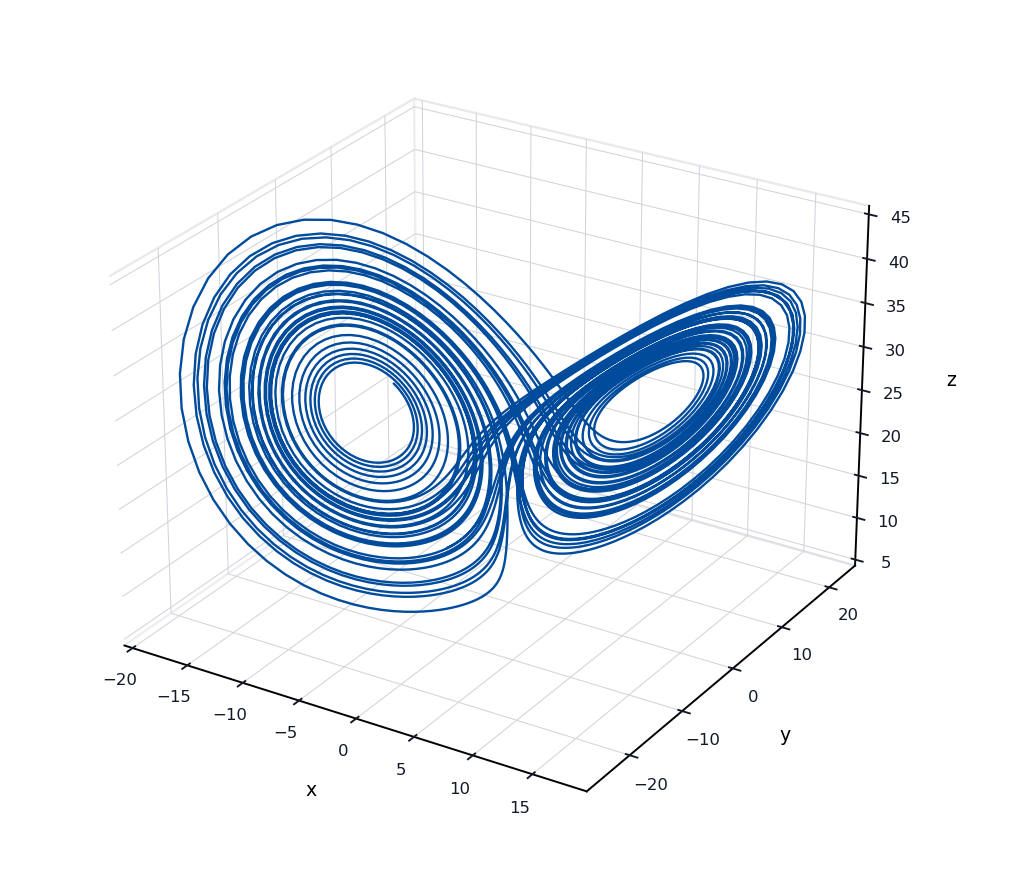
\includegraphics[width=\linewidth]{lorenz_attractor.png}
  \caption{Órbita proyectada en tres dimensiones.}
\end{subfigure}\hfill
\begin{subfigure}[t]{0.62\textwidth}
  \centering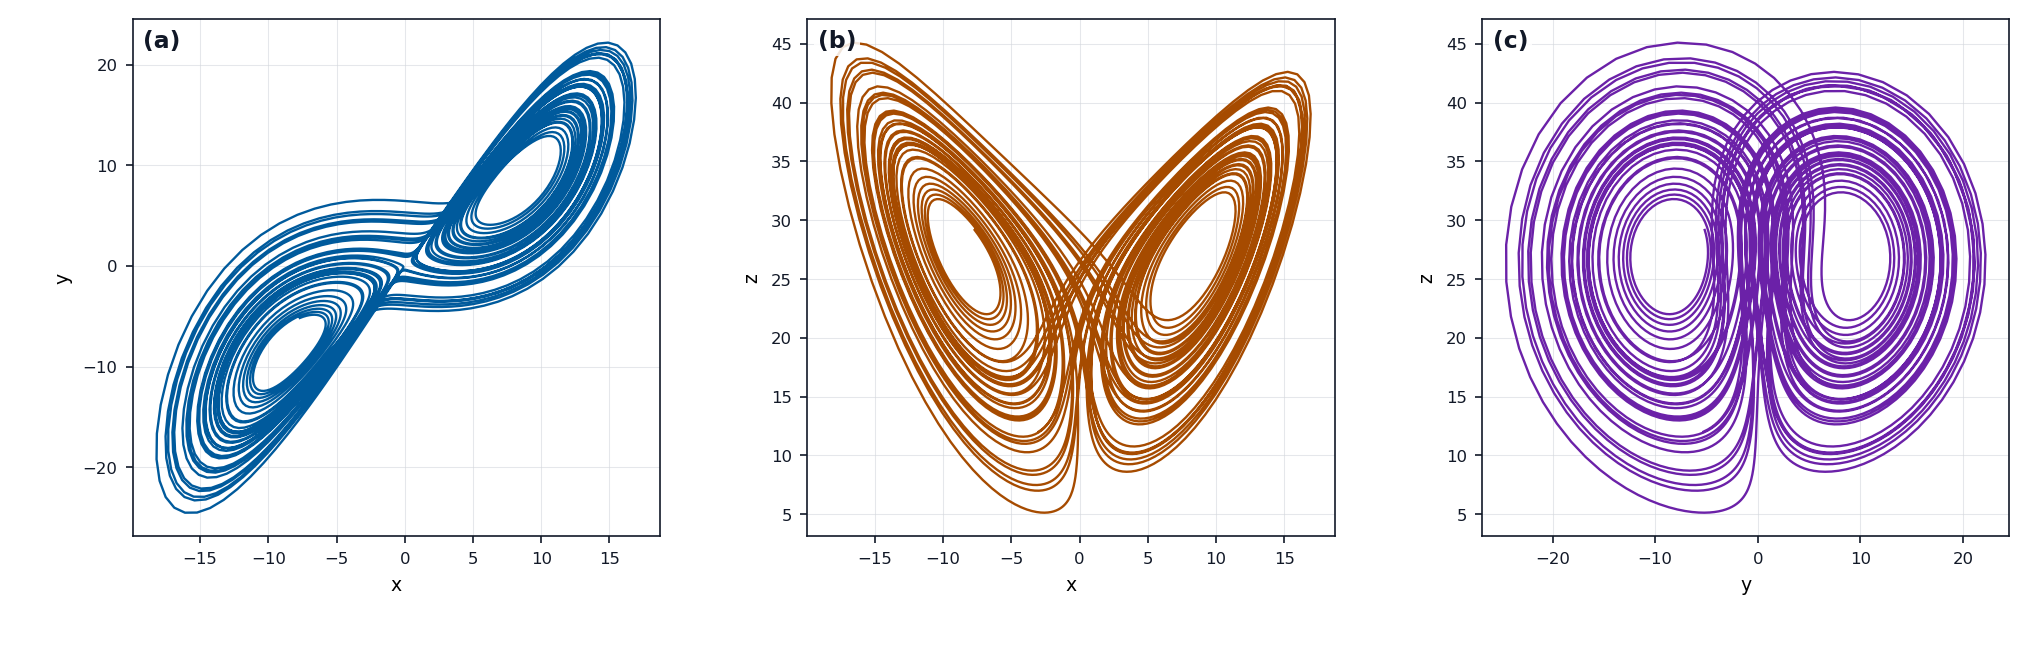
\includegraphics[width=\linewidth]{lorenz_phase_portraits_2d_grid.png}
  \caption{Tres proyecciones del mismo conjunto de estados.}
\end{subfigure}
\caption{Una representación geométrica debe leerse junto con las coordenadas que conserva.}
\label{fig:state-orbit}
\end{figure}

De estas representaciones puede describirse la región visitada, la simetría visible y
la relación entre
coordenadas. La caracterización de caos, atracción y dimensión requiere diagnósticos
adicionales a la forma complicada de la curva. Un cruce en una proyección requiere verificar la intersección en el espacio de estados.

Como primera comprobación, genere una trayectoria de Lorenz y use exactamente los
mismos datos en las tres
pestañas. Identifique un cruce aparente en un retrato 2D y compruebe en la vista 3D
que las alturas $z$ son distintas; después explique en dos frases qué información
recuperó.

\subsection{Flujos y mapas}

Los sistemas de tiempo continuo y discreto requieren procedimientos propios. Un flujo
asigna un estado a cada instante, mientras que un mapa genera una sucesión después de
aplicar repetidamente su regla. Ambos producen órbitas y sus nociones de tiempo
determinan herramientas numéricas específicas.

Formalmente, un flujo autónomo satisface
\[
  \dot{\mathbf{x}}=\mathbf{f}(\mathbf{x};\boldsymbol\mu),\qquad
  \Phi_{t+s}=\Phi_t\circ\Phi_s .
\]
Un mapa iterado satisface
\[
  \mathbf{x}_{n+1}=F(\mathbf{x}_n;\boldsymbol\mu),\qquad F^{n+m}=F^n\circ F^m .
\]
En un flujo, $h$ es un paso de aproximación temporal. En un mapa, $n\mapsto n+1$
es parte del modelo: insertar RK4 entre dos iteraciones cambiaría el sistema.

Esta diferencia determina el cálculo que ejecuta Toolbox Chaos: el selector de sistema
indica si el motor realiza una integración o una iteración.
Para un mapa, la duración representa un número de iteraciones útiles; para un flujo,
los controles de método, $h$ y tiempo final definen una discretización numérica.

Por ejemplo, en el mapa logístico
\[
  x_{n+1}=r x_n(1-x_n),\qquad 0\le x_n\le1,
\]
una órbita de período dos alterna entre dos valores. En un flujo tridimensional, un
ciclo límite es una curva cerrada recorrida continuamente. Ambos son periódicos y
presentan geometrías y procedimientos de observación propios \cite{may1976,devaney1989}.

De este contraste puede compararse la sucesión de estados y su régimen asintótico
dentro del modelo
correcto. El índice $n$ representa iteraciones y el análisis de error de integración corresponde a los flujos; las reglas discretas requieren control de redondeo y sensibilidad a la precisión finita.

Para comprobarlo, simule el mapa logístico con $r=3.2$ y después con $r=3.9$.
Descarte las primeras
500 iteraciones y cuente cuántos valores distintos se distinguen en la cola. Compare
con una órbita periódica de un flujo y escriba la diferencia entre ``período dos'' y
``ciclo límite''.

\subsection{Equilibrios, Jacobiano y estabilidad local}

El análisis de equilibrios relaciona la estabilidad local con el Jacobiano y obliga a
distinguir una conclusión local de una afirmación sobre la dinámica global. Un
equilibrio es un estado donde el campo vectorial se anula. Para estudiar su entorno,
se aproxima la superficie no lineal por su plano tangente.
Los autovalores resumen las direcciones de contracción, expansión y giro de esa
aproximación.

Así, un equilibrio $\mathbf{x}^*$ cumple $\mathbf f(\mathbf{x}^*)=\mathbf 0$. Con
$\boldsymbol\xi=\mathbf{x}-\mathbf{x}^*$, la linealización es
\[
  \dot{\boldsymbol\xi}=J(\mathbf{x}^*)\boldsymbol\xi+O(\|\boldsymbol\xi\|^2),
  \qquad J_{ij}=\frac{\partial f_i}{\partial x_j}.
\]
Si todos los autovalores tienen parte real negativa, el equilibrio hiperbólico es
localmente asintóticamente estable. Una parte real positiva produce una dirección
inestable. Signos mezclados producen una silla. Cuando alguna parte real es cero, la
linealización sola puede ser inconclusa \cite{strogatz2024}.

Para un mapa, la regla cambia: la estabilidad local de un punto fijo requiere

\[
  |\lambda_i(DF(\mathbf{x}^*))|<1
\]
para todos los multiplicadores.

En la pestaña \gui{Autovalores}, el botón
\gui{Calcular equilibrios y autovalores} muestra los
equilibrios disponibles y ubica los autovalores en el plano complejo. El eje vertical
representa la parte imaginaria y el horizontal la parte real. Seleccione cada
equilibrio por separado antes de comparar clasificaciones.

Como referencia, Lorenz tiene el equilibrio $E_0=(0,0,0)$ y, para $\rho>1$, dos
equilibrios
simétricos
\[
  E_\pm=(\pm\sqrt{\beta(\rho-1)},\,\pm\sqrt{\beta(\rho-1)},\,\rho-1).
\]
Al variar $\rho$, sus autovalores cambian. La aparición de una pareja compleja con
parte real positiva describe inestabilidad espiral local. La existencia de un atractor
caótico requiere además análisis de trayectorias y cuencas.

\begin{figure}[H]
\centering
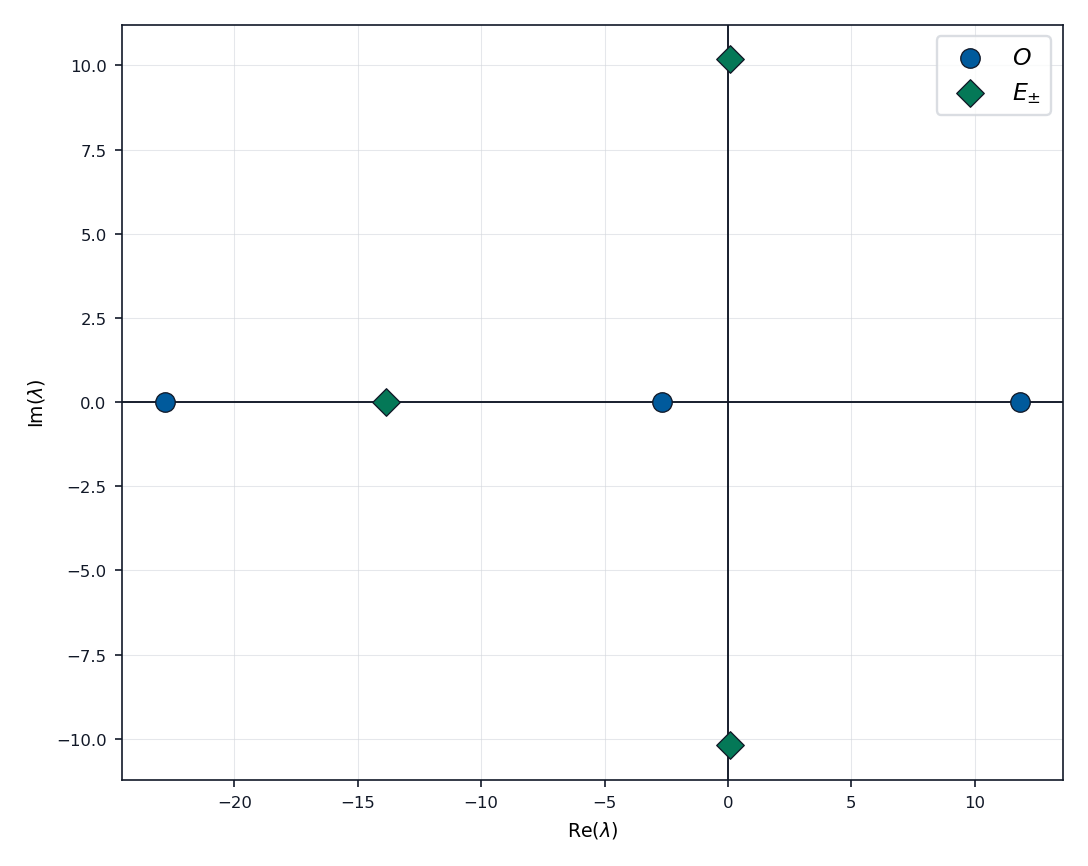
\includegraphics[width=0.68\textwidth]{lorenz_spectrum.png}
\caption{Plano complejo de autovalores. La posición respecto del eje imaginario guía
la lectura local; el análisis global incorpora órbitas y cuencas.}
\label{fig:eigenvalues}
\end{figure}

El resultado permite clasificar la estabilidad local de equilibrios hiperbólicos. La
forma completa de una cuenca, la coexistencia de atractores y la estabilidad global
requieren además análisis de órbitas, regiones invariantes y condiciones iniciales.

\begin{activitybox}{Autovalores y comportamiento lejos del equilibrio}
Calcule los autovalores de Lorenz para dos valores de $\rho$. Dibuje a mano el
semiplano estable y explique qué autovalor cambia la interpretación. Después genere
una trayectoria desde dos condiciones iniciales: contraste y distinga el diagnóstico
local del comportamiento observado lejos del equilibrio.
\end{activitybox}

% Fundamentos ampliados. Se incluye desde manual_teorico_pedagogico.tex.

\section{Modelado, estabilidad y plano de fases}

\begin{objectivebox}
Construir la base analítica que debe preceder a cualquier diagnóstico de caos:
formulación y escalamiento de modelos, dinámica unidimensional, clasificación lineal
plana, linealización no lineal, nullclines, ciclos límite y bifurcaciones locales.
Cada tema termina con un cálculo reproducible en Toolbox Chaos y con una delimitación
explícita de la evidencia que aporta la gráfica y de la que exige cálculos adicionales.
\end{objectivebox}

\subsection{Modelado, variables de estado y adimensionalización}

\paragraph{Variables de estado y escalas.}
Un \term{modelo dinámico} especifica un estado \(\mathbf{x}\), parámetros
\(\boldsymbol\mu\), una ley de evolución y las hipótesis bajo las cuales esa ley es
válida. Elegir el estado incorpora las variables observables y la
información necesaria para continuar el movimiento. Por ejemplo, la posición de una
masa requiere también su velocidad. La forma de primer orden de una
ecuación de orden \(k\) amplía el estado hasta contener las derivadas requeridas.

La \term{adimensionalización} introduce escalas características y reemplaza
magnitudes con unidad por cocientes sin dimensión. Esto reduce el número de
parámetros independientes, permite comparar experimentos de distinta escala y evita
interpretar como esencial un valor que depende de la unidad elegida. Esta
operación identifica las razones físicas que controlan el régimen.

\paragraph{Ecuación dimensional y transformación.}
Considérese el oscilador de Duffing forzado
\[
 m\ddot x+c\dot x+kx+\alpha x^3=F\cos(\Omega t),
 \qquad m>0,\quad k>0.
\]
Se eligen
\[
 \omega_0=\sqrt{\frac{k}{m}},\qquad
 \tau=\omega_0t,\qquad x=L u,\qquad
 L=\sqrt{\frac{k}{|\alpha|}}.
\]
Como \(\dot x=L\omega_0u'\) y
\(\ddot x=L\omega_0^2u''\), al dividir entre \(kL\) resulta
\[
 u''+2\zeta u'+u+s u^3=f\cos(\nu\tau),
\]
donde las primas representan derivación respecto de \(\tau\) y
\[
 \zeta=\frac{c}{2\sqrt{mk}},\qquad
 s=\operatorname{sgn}(\alpha),\qquad
 f=\frac{F}{kL},\qquad
 \nu=\frac{\Omega}{\omega_0}.
\]
Los cinco parámetros dimensionales \(m,c,k,\alpha,F,\Omega\) quedan organizados en
cuatro combinaciones que separan amortiguamiento, signo de la rigidez cúbica,
intensidad y frecuencia relativa del forzamiento.

\paragraph{Ejemplo de adimensionalización.}
Sea \(m=1\), \(k=4\), \(c=0.8\), \(\alpha=2\), \(F=1\) y \(\Omega=3\), en unidades
compatibles. Entonces
\[
 \omega_0=2,\qquad L=\sqrt2,\qquad
 \zeta=\frac{0.8}{2(2)}=0.2,\qquad
 s=1,
\]
\[
 f=\frac{1}{4\sqrt2}\simeq0.1767767,\qquad
 \nu=\frac32.
\]
La ecuación adimensional queda
\[
 u''+0.4u'+u+u^3=0.1767767\cos(1.5\tau).
\]
Para convertirla en un flujo autónomo se define \(v=u'\) y una fase
\(\phi=\nu\tau\):
\[
 u'=v,\qquad
 v'=-0.4v-u-u^3+0.1767767\cos\phi,\qquad
 \phi'=1.5.
\]
La fase crece sin cota, pero el forzamiento depende de ella módulo \(2\pi\). Una
sección \(\phi=0\pmod{2\pi}\) produce el mapa estroboscópico del oscilador.

\begin{activitybox}{Práctica reproducible: Duffing adimensional}
Abra \gui{Crear sistema}. Use las variables \texttt{u, v, phi}; parámetros
\texttt{zeta=0.2}, \texttt{s=1}, \texttt{f=0.176776695},
\texttt{nu=1.5}; y ecuaciones, en ese orden,
\texttt{v},
\texttt{-2*zeta*v-u-s*u**3+f*cos(phi)} y \texttt{nu}.
Use estado inicial \((0.1,0,0)\), método RK4, paso \(h=0.005\), duración \(200\),
5000 muestras transitorias y umbral de divergencia \(10^6\). Pulse
\gui{Validar definicion} y \gui{Simular y graficar}; después reutilice la trayectoria
en \gui{Retratos 2D} y \gui{Series temporales}. Repita con \(h=0.0025\).
\end{activitybox}

\paragraph{Lectura de las variables escaladas.}
En \(u(\tau)\) se observan transitorio, amplitud y modulación; en el retrato
\((u,v)\), rotación, deformación por el término cúbico y posible acercamiento a un
régimen. La fase representa la variable que hace autónomo el forzamiento y se integra
en el estado ampliado del sistema. Dos trayectorias que se separan tarde pueden
conservar amplitudes, sección estroboscópica y distribución semejantes.

\begin{warningbox}
La validación de hipótesis físicas requiere su contraste experimental o teórico, y la
existencia de un atractor requiere evidencia adicional a una trayectoria acotada. La
comparación entre \(u\) y \(x\) incorpora el factor \(L\), mientras que la fase creciente
se interpreta mediante el forzamiento periódico del oscilador.
\end{warningbox}

\lecturaseccion{Robert C. Hilborn, \emph{Chaos and Nonlinear Dynamics: An
Introduction for Scientists and Engineers}, 2.\textsuperscript{a} ed., capítulo 3,
``An Introduction to Flows'', y apéndice G, ``The Duffing Oscillator''; Tamás Tél y
Márton Gruiz, \emph{Chaotic Dynamics: An Introduction Based on Classical Mechanics},
apéndice A, apartados sobre ecuaciones adimensionales, integración de EDO y programas
de ejemplo; Frank C. Hoppensteadt, \emph{Analysis and Simulation of Chaotic Systems},
2.\textsuperscript{a} ed., sección 6.2, apartados sobre Duffing y simulación.}

\subsection{Flujos de una dimensión, potenciales y formas normales}

\paragraph{Campo vectorial en una dimensión.}
Un flujo autónomo unidimensional tiene la forma
\[
 \dot x=f(x;\mu).
\]
Los equilibrios satisfacen \(f(x^*;\mu)=0\). Entre dos ceros consecutivos, la
continuidad de \(f\) mantiene su signo: \(f>0\) orienta la línea de fase hacia la
derecha y \(f<0\) hacia la izquierda. Si el equilibrio es hiperbólico,
\[
 f_x(x^*;\mu)<0\ \Longrightarrow\ \text{estable},\qquad
 f_x(x^*;\mu)>0\ \Longrightarrow\ \text{inestable}.
\]
La unicidad impide que dos soluciones distintas se crucen y descarta órbitas
periódicas no constantes en la recta.

\paragraph{Representación mediante potencial.}
Toda ecuación escalar puede escribirse formalmente como
\[
 \dot x=-\frac{\mathrm dV}{\mathrm dx},
 \qquad
 V(x)=-\int^x f(s)\,\mathrm ds.
\]
A lo largo de una solución,
\[
 \frac{\mathrm dV}{\mathrm dt}=V'(x)\dot x=-[f(x)]^2\leq0.
\]
Los mínimos locales de \(V\) corresponden a equilibrios estables; los máximos, a
inestables. Su extensión a un sistema general de varias dimensiones requiere una
justificación específica.

\paragraph{Ejemplo algebraico resuelto: saddle--node.}
Para
\[
 \dot x=\mu-x^2
\]
y \(\mu=1/4\), los equilibrios son \(x_\pm=\pm1/2\). Como
\(f_x=-2x\),
\[
 f_x(-1/2)=1>0,\qquad f_x(1/2)=-1<0.
\]
Por tanto, \(x_-=-1/2\) es inestable y \(x_+=1/2\) estable. El potencial
\[
 V(x)=\frac{x^3}{3}-\mu x
\]
tiene un máximo en \(-1/2\) y un mínimo en \(1/2\). Para \(\mu=0\) ambos puntos
colisionan en \(x=0\), donde \(f_x=0\) y la prueba lineal es inconclusa; para
\(\mu<0\) ya no hay equilibrio real.

\paragraph{Las tres formas normales escalares.}
\begin{longtable}{>{\raggedright\arraybackslash}p{0.23\linewidth}
                  >{\raggedright\arraybackslash}p{0.27\linewidth}
                  >{\raggedright\arraybackslash}p{0.40\linewidth}}
\toprule
Mecanismo & Forma normal & Ramas y cambio cualitativo \\
\midrule
\endhead
Saddle--node & \(\dot x=\mu-x^2\) &
Ninguna rama para \(\mu<0\); dos ramas \(x=\pm\sqrt\mu\) para \(\mu>0\).\\
Transcrítica & \(\dot x=\mu x-x^2\) &
Las ramas \(x=0\) y \(x=\mu\) intercambian estabilidad en \(\mu=0\).\\
Pitchfork supercrítica & \(\dot x=\mu x-x^3\) &
\(x=0\) pierde estabilidad y nacen \(x=\pm\sqrt\mu\) estables para \(\mu>0\).\\
\bottomrule
\end{longtable}
Estas ecuaciones son representantes locales después de cambios de coordenadas y
escalas; su uso en un sistema real requiere establecer las hipótesis que conducen a esos polinomios.

\begin{activitybox}{Práctica reproducible: líneas de fase}
En \gui{Crear sistema}, defina una variable \texttt{x}, un parámetro
\texttt{mu} y la ecuación \texttt{mu-x**2}. Para
\(\mu=-0.25,0,0.25\), use los estados iniciales
\(-1,-0.6,-0.4,0,0.4,0.6,1\), paso \(h=0.01\) y duración \(20\).
Guarde las series en escalas separadas. Repita para
\texttt{mu*x-x**2} y \texttt{mu*x-x**3}; antes de simular, dibuje sus ramas y
prediga el destino de cada condición.
\end{activitybox}

\paragraph{Lectura de potenciales y retratos lineales.}
En una serie temporal, la aproximación monótona a un nivel concuerda con una flecha
de la línea de fase; el escape rápido indica que el intervalo y el modelo deben
revisarse. Cerca de una bifurcación aparece \term{ralentización crítica}: la tasa
lineal es pequeña y el transitorio puede ser mucho más largo. Una gráfica contra
\(\mu\) debe distinguir ramas estables e inestables; las ramas inestables requieren
continuación o estados iniciales controlados para su representación.

\begin{warningbox}
Un equilibrio requiere un criterio de convergencia y una rama requiere continuación o
barridos de parámetros que la localicen. En un
punto no hiperbólico \(f'(x^*)=0\), el análisis conserva términos no lineales o
incorpora un estudio de signos.
\end{warningbox}

\lecturaseccion{Steven H. Strogatz, \emph{Nonlinear Dynamics and Chaos with
Applications to Physics, Biology, Chemistry, and Engineering},
2.\textsuperscript{a} ed., secciones 2.1--2.4, 2.7--2.8 y 3.1--3.6; Morris W.
Hirsch, Stephen Smale y Robert L. Devaney, \emph{Differential Equations, Dynamical
Systems, and an Introduction to Chaos}, 3.\textsuperscript{a} ed., capítulo 1,
apartados sobre ecuación logística, cosecha y bifurcaciones.}

\subsection{Sistemas lineales planos y plano traza--determinante}

\paragraph{Matriz del sistema y solución espectral.}
Para el sistema homogéneo
\[
 \dot{\mathbf x}=A\mathbf x,\qquad
 A=\begin{pmatrix}a&b\\c&d\end{pmatrix},
\]
la solución es \(\mathbf x(t)=e^{At}\mathbf x_0\). Los autovalores satisfacen
\[
 p(\lambda)=\lambda^2-\tau\lambda+\Delta=0,\qquad
 \tau=a+d,\quad \Delta=ad-bc.
\]
Así,
\[
 \lambda_{\pm}=\frac{\tau\pm\sqrt{\tau^2-4\Delta}}{2}.
\]
El signo de \(\Delta\) detecta una silla cuando es negativo. Si \(\Delta>0\), el
signo de \(\tau\) decide atracción o repulsión y el discriminante
\(\mathcal D=\tau^2-4\Delta\) separa autovalores reales de complejos.

\paragraph{Clasificación algebraica.}
\begin{longtable}{>{\raggedright\arraybackslash}p{0.27\linewidth}
                  >{\raggedright\arraybackslash}p{0.28\linewidth}
                  >{\raggedright\arraybackslash}p{0.35\linewidth}}
\toprule
Condición & Tipo hiperbólico & Lectura local \\
\midrule
\endhead
\(\Delta<0\) & Silla & Una dirección entra y otra sale.\\
\(\Delta>0,\ \mathcal D>0,\ \tau<0\) & Nodo estable & Dos tasas reales de
contracción.\\
\(\Delta>0,\ \mathcal D>0,\ \tau>0\) & Nodo inestable & Dos tasas reales de
expansión.\\
\(\Delta>0,\ \mathcal D<0,\ \tau<0\) & Foco estable & Rotación con contracción.\\
\(\Delta>0,\ \mathcal D<0,\ \tau>0\) & Foco inestable & Rotación con expansión.\\
\(\tau=0,\ \Delta>0\) & Centro lineal & Órbitas periódicas neutrales en el sistema
lineal.\\
\bottomrule
\end{longtable}
Las fronteras \(\Delta=0\) y \(\mathcal D=0\) contienen casos degenerados; la recta
\(\tau=0\) requiere especial cuidado en problemas no lineales.

\paragraph{Ejemplo de clasificación por traza y determinante.}
Sea
\[
 A=\begin{pmatrix}-1&2\\-2&-1\end{pmatrix}.
\]
Entonces \(\tau=-2\), \(\Delta=5\) y
\(\mathcal D=4-20=-16\), de modo que
\(\lambda_\pm=-1\pm2i\): el origen es un foco estable. Además,
\[
 \frac{\mathrm d}{\mathrm dt}(x^2+y^2)
 =2x(-x+2y)+2y(-2x-y)=-2(x^2+y^2),
\]
por lo que \(r(t)=r_0e^{-t}\). La velocidad angular es
\[
 \dot\theta=\frac{x\dot y-y\dot x}{x^2+y^2}=-2.
\]
La órbita gira en sentido horario, con periodo angular \(\pi\), mientras su radio
decrece exponencialmente. Este cálculo explica tanto la forma como la orientación.

\begin{activitybox}{Práctica reproducible: atlas de sistemas lineales}
En \gui{Crear sistema}, use variables \texttt{x, y} y ecuaciones \texttt{a*x+b*y},
\texttt{c*x+d*y}. Ejecute: silla \((a,b,c,d)=(1,0,0,-1)\); nodo estable
\((-1,0,0,-2)\); centro \((0,-1,1,0)\); y foco estable
\((-1,2,-2,-1)\). Use condiciones \((1,0)\), \((0,1)\), \((1,1)\) y
\((-1,1)\), RK4, \(h=0.01\), \(T=15\). Reutilice cada trayectoria en
\gui{Retratos 2D} y verifique sentido de giro y tasas.
\end{activitybox}

\paragraph{Lectura del plano traza--determinante.}
En un nodo, las órbitas se alinean con la dirección propia de contracción más lenta;
en una silla, salvo sobre la variedad estable, terminan dominadas por la dirección
inestable. En un foco, el espacio entre vueltas cambia exponencialmente. Una escala
automática puede ocultar esa contracción: conviene fijar límites comparables o usar
también \(r(t)\).

\begin{warningbox}
El plano traza--determinante clasifica matrices reales \(2\times2\). El análisis de
sistemas de otra dimensión requiere herramientas acordes con su Jacobiano. Un centro
lineal requiere términos de orden superior para determinar si aparece una espiral débil
o un ciclo límite, y la orientación de giro se obtiene del campo completo además de
\(\tau\) y \(\Delta\).
\end{warningbox}

\lecturaseccion{Morris W. Hirsch, Stephen Smale y Robert L. Devaney,
\emph{Differential Equations, Dynamical Systems, and an Introduction to Chaos},
3.\textsuperscript{a} ed., capítulos 2--4, con énfasis en retratos y clasificación
traza--determinante; Steven H. Strogatz, \emph{Nonlinear Dynamics and Chaos with
Applications to Physics, Biology, Chemistry, and Engineering},
2.\textsuperscript{a} ed., secciones 5.1--5.2.}

\subsection{Jacobiano, linealización y nullclines}

\paragraph{Jacobiano, linealización y nullclines.}
Para
\[
 \dot x=f(x,y),\qquad \dot y=g(x,y),
\]
las \term{nullclines} son los conjuntos \(f=0\) y \(g=0\). Sobre la primera, el
vector es vertical; sobre la segunda, horizontal. Sus intersecciones son equilibrios.
El \term{Jacobiano}
\[
 J(x,y)=
 \begin{pmatrix}
 f_x&f_y\\g_x&g_y
 \end{pmatrix}
\]
produce la aproximación
\(\dot{\boldsymbol\xi}=J(x^*,y^*)\boldsymbol\xi+O(\|\boldsymbol\xi\|^2)\).
Si el equilibrio es hiperbólico, la clasificación lineal conserva la estructura
local cualitativa; si algún autovalor tiene parte real cero, se requieren criterios adicionales.

\paragraph{Ejemplo de Jacobiano y puntos críticos.}
Considérese
\[
 \dot x=x(1-x-y),\qquad
 \dot y=y\left(x-\frac12\right).
\]
Las nullclines son
\[
 x=0\ \text{o}\ y=1-x,\qquad
 y=0\ \text{o}\ x=\frac12.
\]
Sus intersecciones relevantes son
\[
 E_0=(0,0),\qquad E_1=(1,0),\qquad E_c=(1/2,1/2).
\]
El Jacobiano es
\[
 J(x,y)=
 \begin{pmatrix}
 1-2x-y&-x\\
 y&x-\tfrac12
 \end{pmatrix}.
\]
En \(E_0\), \(J=\operatorname{diag}(1,-1/2)\): es una silla. En \(E_1\),
\[
 J(E_1)=\begin{pmatrix}-1&-1\\0&1/2\end{pmatrix},
\]
también una silla. En \(E_c\),
\[
 J(E_c)=
 \begin{pmatrix}-1/2&-1/2\\1/2&0\end{pmatrix},
\quad
 \tau=-\frac12,\quad\Delta=\frac14,\quad
 \mathcal D=-\frac34.
\]
Los autovalores son
\[
 \lambda_\pm=-\frac14\pm i\frac{\sqrt3}{4},
\]
así que el equilibrio de coexistencia es un foco estable local.

\paragraph{Campo de signos.}
En el primer cuadrante, \(x\) aumenta debajo de \(y=1-x\) y disminuye encima;
\(y\) aumenta a la derecha de \(x=1/2\) y disminuye a la izquierda. Esta tabla de
signos predice el giro alrededor de \(E_c\) antes de integrar. También muestra que los
ejes son invariantes porque los factores \(x\) y \(y\) impiden cruzarlos desde datos
positivos.

\begin{activitybox}{Práctica reproducible: nullclines y linealización}
En \gui{Crear sistema}, use variables \texttt{x, y} y ecuaciones
\texttt{x*(1-x-y)} y \texttt{y*(x-0.5)}. Simule con RK4,
\(h=0.01\), \(T=60\), desde \((0.1,0.1)\), \((0.9,0.1)\), \((0.2,0.8)\),
\((0.8,0.8)\), \((1.4,0.2)\) y \((0.4,1.2)\). En una copia del retrato, dibuje las
cuatro nullclines y marque los tres equilibrios. Compare la orientación numérica con
la tabla de signos y repita una trayectoria con \(h/2\).
\end{activitybox}

\paragraph{Lectura del campo y las nullclines.}
Las órbitas cruzan una nullcline con tangente vertical u horizontal, salvo en un
equilibrio. Cerca de \(E_c\), la espiral observada debe contraerse con tasa compatible
con \(\Re\lambda=-1/4\); lejos de él, la curvatura depende del campo completo. Las
separatrices de las sillas organizan regiones del plano; una trayectoria
numérica genérica aproxima esa variedad unidimensional con una precisión dependiente del integrador.

\begin{warningbox}
Una nullcline localiza donde una componente de la velocidad se anula; la trayectoria y
las barreras invariantes se determinan a partir del campo completo. El Jacobiano informa
en una vecindad del equilibrio, mientras que la descripción de cuencas globales y coexistencia exige
la evidencia correspondiente sobre ciclos. Cuando el estado simulado abandona el dominio físico,
la revisión del modelo incorpora esa salida y la conserva visible en la gráfica.
\end{warningbox}

\lecturaseccion{Morris W. Hirsch, Stephen Smale y Robert L. Devaney,
\emph{Differential Equations, Dynamical Systems, and an Introduction to Chaos},
3.\textsuperscript{a} ed., capítulo 8, secciones 8.1--8.5, y capítulo 9, apartados
sobre nullclines, estabilidad, sistemas gradiente y hamiltonianos; Steven H.
Strogatz, \emph{Nonlinear Dynamics and Chaos with Applications to Physics, Biology,
Chemistry, and Engineering}, 2.\textsuperscript{a} ed., secciones 6.1--6.3 y 6.8.}

\subsection{Osciladores, ciclos límite y Poincaré--Bendixson}

\paragraph{Ciclos límite y osciladores planos.}
Una \term{órbita periódica} satisface
\(\mathbf x(t+T)=\mathbf x(t)\) para algún \(T>0\). Un \term{ciclo límite} es una
órbita periódica aislada: las órbitas cercanas pueden aproximarse a ella o alejarse.
Un centro lineal, en cambio, posee una familia continua de órbitas cerradas y ninguna
es aislada.

El teorema de Poincaré--Bendixson, en una formulación útil, afirma que si una órbita
de un flujo plano permanece en una región compacta, su conjunto límite no contiene
equilibrios y se satisfacen las hipótesis regulares, entonces dicho conjunto es una
órbita periódica. El teorema delimita los comportamientos posibles al excluir caos determinista sostenido
en flujos autónomos suaves de dos dimensiones, pero exige demostrar acotación y
ausencia de equilibrios en el conjunto límite.

\paragraph{Ejemplo algebraico resuelto: normal radial.}
Considérese
\[
 \dot x=(1-x^2-y^2)x-y,\qquad
 \dot y=x+(1-x^2-y^2)y.
\]
Con \(r^2=x^2+y^2\),
\[
 \dot r=\frac{x\dot x+y\dot y}{r}=r(1-r^2),\qquad
 \dot\theta=\frac{x\dot y-y\dot x}{r^2}=1.
\]
Los radios equilibrados son \(r=0\) y \(r=1\). Como
\[
 g'(r)=1-3r^2,\qquad g'(0)=1,\qquad g'(1)=-2,
\]
el origen es inestable y el círculo \(r=1\) es un ciclo límite estable. El periodo es
\(T=2\pi\). Para una perturbación radial pequeña \(\eta=r-1\),
\(\dot\eta\simeq-2\eta\), de modo que el multiplicador aproximado de retorno es
\[
 M=e^{-2T}=e^{-4\pi}<1.
\]
Esto cuantifica la atracción transversal y la distingue de la contracción a un punto.

\paragraph{Exclusión de ciclos.}
Si la divergencia
\[
 \nabla\cdot\mathbf f=f_x+g_y
\]
mantiene signo estricto en una región simplemente conexa, el criterio de
Bendixson--Dulac excluye órbitas periódicas contenidas en ella. Un signo que cambia
requiere un criterio adicional para decidir la existencia de un ciclo.

\begin{activitybox}{Práctica reproducible: ciclo estable y periodo}
En \gui{Crear sistema}, use variables \texttt{x, y} y ecuaciones
\texttt{(1-x**2-y**2)*x-y} y
\texttt{x+(1-x**2-y**2)*y}. Elija puntos con radios \(0.2,0.8,1.2,2\), por ejemplo
\((0.2,0)\), \((0.8,0)\), \((1.2,0)\), \((2,0)\). Integre con RK4,
\(h=0.01\), \(T=30\). En \gui{Series temporales}, estime el periodo con diez máximos;
en \gui{Retratos 2D}, compruebe acercamiento desde dentro y fuera. Repita con
\(h=0.005\) y compare periodo y radio medio de las últimas cinco vueltas.
\end{activitybox}

\paragraph{Lectura de ciclos límite.}
Una espiral que se acumula sobre una curva cerrada sugiere atracción orbital. La serie
temporal permite comprobar amplitud y periodo; el retrato muestra aislamiento. Para
una evidencia más directa se fija una sección transversal y se grafica
\(r_{n+1}\) contra \(r_n\): un cruce con la diagonal y pendiente de módulo menor que
uno corresponde a un punto fijo estable del mapa de retorno.

\begin{warningbox}
Una curva cerrada trazada con pocas muestras puede ser un polígono numérico. Observar
varias vueltas exige verificar aislamiento y estabilidad. Poincaré--Bendixson se
aplica directamente a mapas, flujos tridimensionales, campos discontinuos o
proyecciones planas de una órbita 3D.
\end{warningbox}

\lecturaseccion{Steven H. Strogatz, \emph{Nonlinear Dynamics and Chaos with
Applications to Physics, Biology, Chemistry, and Engineering},
2.\textsuperscript{a} ed., secciones 7.2, 7.3, 7.4, 7.5, 7.6 y 8.7; Morris W.
Hirsch, Stephen Smale y Robert L. Devaney, \emph{Differential Equations, Dynamical
Systems, and an Introduction to Chaos}, 3.\textsuperscript{a} ed., capítulo 10,
apartados sobre conjuntos límite, mapas de Poincaré y teorema de
Poincaré--Bendixson, y capítulo 12, apartados sobre Liénard y van der Pol.}

\subsection{Bifurcaciones locales y forma normal de Hopf}

\paragraph{Parámetro y cambio de estabilidad.}
Una \term{bifurcación} es un cambio cualitativo de la dinámica al variar un
parámetro. En una bifurcación local de equilibrio, la linealización pierde
hiperbolicidad: un autovalor real cruza cero o un par complejo conjugado cruza el eje
imaginario. La condición espectral señala el posible punto de bifurcación; las condiciones de
transversalidad y no degeneración deciden si aparece la forma normal genérica.

\paragraph{Mecanismos de bifurcación local.}
\begin{longtable}{>{\raggedright\arraybackslash}p{0.25\linewidth}
                  >{\raggedright\arraybackslash}p{0.30\linewidth}
                  >{\raggedright\arraybackslash}p{0.35\linewidth}}
\toprule
Bifurcación & Firma lineal & Consecuencia de la forma normal \\
\midrule
\endhead
Saddle--node & Un autovalor simple pasa por \(0\) &
Creación o destrucción de dos equilibrios.\\
Transcrítica & Un autovalor pasa por \(0\), con ramas preexistentes &
Dos ramas intercambian estabilidad.\\
Pitchfork & Autovalor \(0\) y simetría apropiada &
Una rama simétrica se divide o se reúne.\\
Hopf & \(\lambda_{1,2}(\mu)=\alpha(\mu)\pm i\omega(\mu)\),
\(\alpha(0)=0\), \(\omega(0)\ne0\) &
Nace o muere un ciclo pequeño; su estabilidad depende del término cúbico.\\
\bottomrule
\end{longtable}

\paragraph{Ejemplo algebraico resuelto: Hopf supercrítica.}
La ecuación compleja
\[
 \dot z=(\mu+i\omega)z-|z|^2z,\qquad \omega>0,
\]
equivale, con \(z=re^{i\theta}\), a
\[
 \dot r=\mu r-r^3,\qquad \dot\theta=\omega.
\]
En el origen, los autovalores son \(\mu\pm i\omega\). Para \(\mu<0\), el origen es
estable y no hay radio positivo equilibrado. Para \(\mu>0\), el origen es inestable
y aparece
\[
 r_*=\sqrt{\mu},\qquad T=\frac{2\pi}{\omega}.
\]
Como \(\partial_r(\mu r-r^3)|_{r_*}=\mu-3\mu=-2\mu<0\), el ciclo es estable. Si
\(\mu=0.09\) y \(\omega=2\), entonces \(r_*=0.3\), \(T=\pi\) y el multiplicador
radial lineal por vuelta es
\[
 M=e^{-2\mu T}=e^{-0.18\pi}\simeq0.568.
\]
La amplitud sigue la ley de escala \(\sqrt\mu\) respecto de \(\mu\).

\begin{activitybox}{Práctica reproducible: cruce de Hopf}
En \gui{Crear sistema}, use variables \texttt{x, y}, parámetros
\texttt{mu} y \texttt{omega=2}, y ecuaciones
\texttt{mu*x-omega*y-(x**2+y**2)*x} y
\texttt{omega*x+mu*y-(x**2+y**2)*y}. Ejecute
\(\mu=-0.09,0,0.09,0.25\) desde \((0.05,0)\) y \((0.8,0)\), con RK4,
\(h=0.005\), \(T=80\). Estime en cada caso el radio tardío y el periodo. Grafique
\(r^2\) contra \(\mu\): la predicción exacta de la forma normal es
\(r^2=\mu\) para \(\mu>0\).
\end{activitybox}

\begin{figure}[H]
\centering
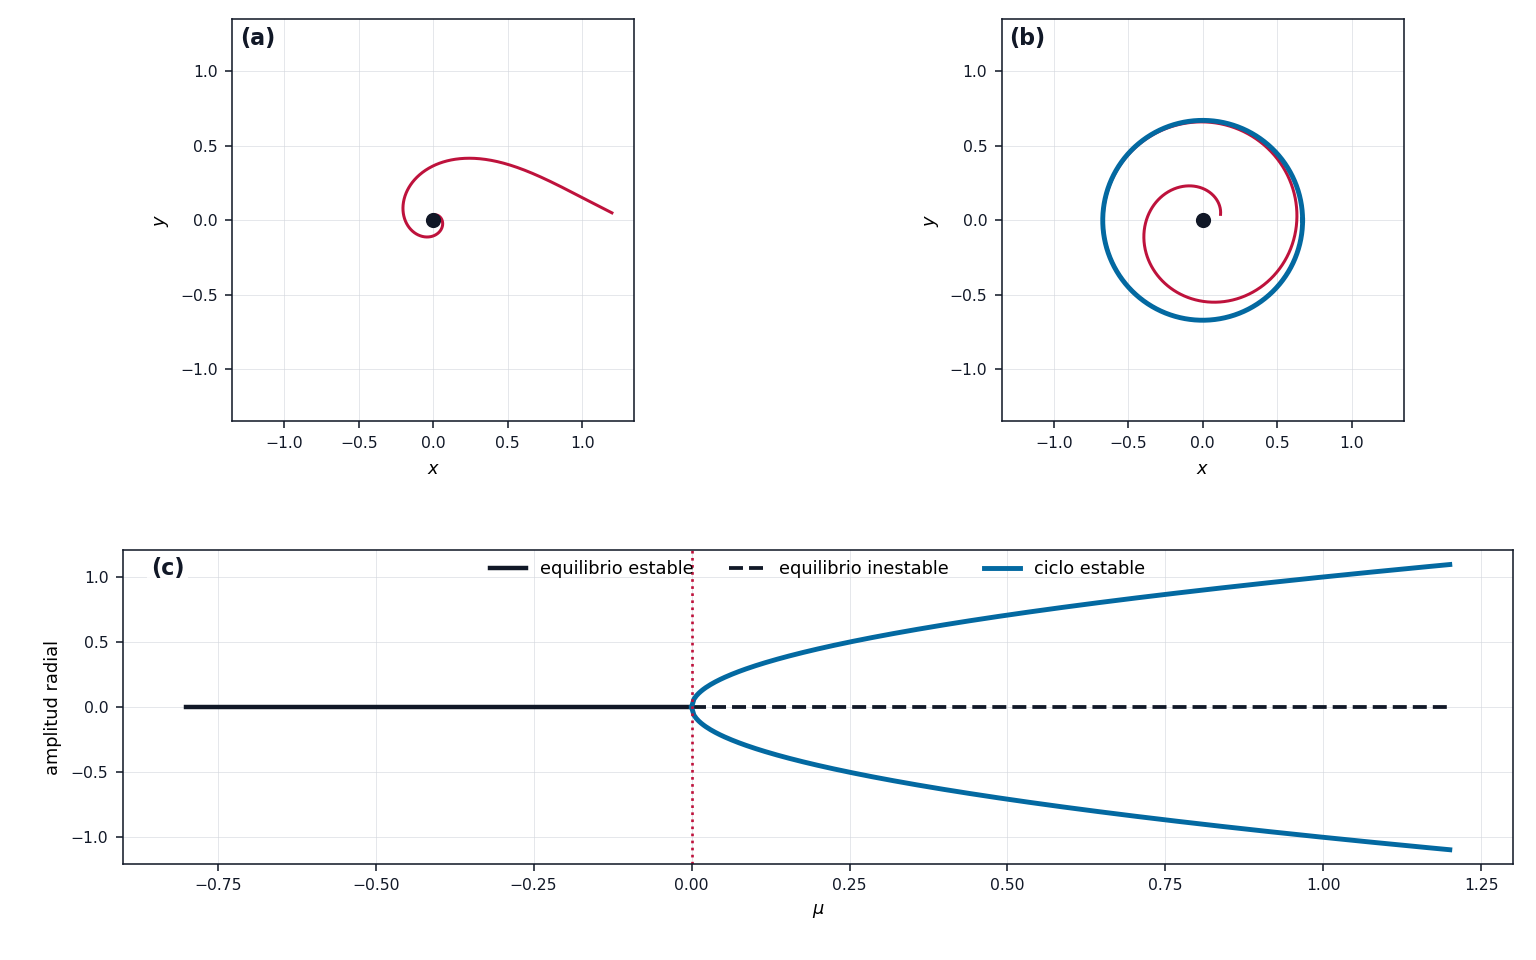
\includegraphics[width=0.78\linewidth]{hopf_bifurcation_example.png}
\caption{Ejemplo generado para Toolbox Chaos de un cambio tipo Hopf. La lectura
correcta combina la estabilidad del equilibrio, la amplitud de la órbita y el
parámetro; la identificación de condiciones de genericidad requiere proyecciones y pruebas adicionales.}
\label{fig:hopf-fundamentos-ampliados}
\end{figure}

\paragraph{Interpretación de la gráfica de bifurcación.}
En un diagrama amplitud--parámetro, la rama \(r=0\) cambia de estabilidad en
\(\mu=0\) y la rama \(r=\sqrt\mu\) nace con tangente vertical. En una simulación, el
tiempo de relajación crece cerca de cero porque la tasa \(|2\mu|\) disminuye. Si el
transitorio se mantiene fijo durante un barrido, ese retraso puede deformar la rama o
hacer parecer que existe histéresis.

\begin{warningbox}
Un par de autovalores con parte real próxima a cero motiva la verificación de una
bifurcación de Hopf mediante cruce transversal, no degeneración y presencia
del ciclo. Un barrido en ambas direcciones distingue transitorio, coexistencia e
histéresis; la estabilidad de una rama requiere un criterio adicional a los estados visitados.
\end{warningbox}

\lecturaseccion{Steven H. Strogatz, \emph{Nonlinear Dynamics and Chaos with
Applications to Physics, Biology, Chemistry, and Engineering},
2.\textsuperscript{a} ed., secciones 3.1--3.6 y 8.1--8.4; John Guckenheimer y Philip
Holmes, \emph{Nonlinear Oscillations, Dynamical Systems, and Bifurcations of Vector
Fields}, capítulo 3, apartados sobre variedades centrales, formas normales y
bifurcaciones locales; Morris W. Hirsch, Stephen Smale y Robert L. Devaney,
\emph{Differential Equations, Dynamical Systems, and an Introduction to Chaos},
3.\textsuperscript{a} ed., sección 8.5, ``Bifurcations'', y capítulo 12, apartado
sobre bifurcación de Hopf.}

\subsection*{Criterios de análisis para sistemas planos}
\addcontentsline{toc}{subsection}{Síntesis operativa de los fundamentos}

\begin{evidencebox}{Cadena mínima antes de hablar de caos}
Primero declare el estado y escale el modelo. Después determine equilibrios,
nullclines y Jacobiano; construya una predicción local y un retrato global; compruebe
el integrador y retire el transitorio. Con esa cadena establecida, calcule
bifurcaciones, exponentes, espectros o dimensiones. Esta secuencia permite
distinguir un mecanismo dinámico de un artefacto de modelado o de discretización.
\end{evidencebox}

\begin{activitybox}{Problema integrador de fundamentos}
Elija un sistema plano propio. Entregue: variables y unidades; forma adimensional;
equilibrios; Jacobiano; clasificación traza--determinante; nullclines; regiones de
signo; una afirmación sobre ciclos basada en Poincaré--Bendixson o Bendixson--Dulac;
cuatro trayectorias reproducibles en \gui{Crear sistema}; y una comparación con
\(h/2\). Termine con dos columnas: ``evidencia disponible'' y ``evidencia adicional requerida''.
\end{activitybox}


\section{Integración numérica, error y transitorios}
\lecturaseccion{Kathleen T. Alligood, Tim D. Sauer y James A. Yorke, \emph{Chaos: An Introduction to Dynamical Systems}, apéndice B; Frank C. Hoppensteadt, \emph{Analysis and Simulation of Chaotic Systems}, capítulos 1--2.}

Para obtener una trayectoria confiable se separan la dinámica del modelo y los
efectos del método, el paso, el redondeo y el intervalo transitorio. Una computadora
construye una cadena de aproximaciones a la curva continua. En un sistema sensible,
dos cálculos correctos pueden perder coincidencia punto a punto después de cierto
tiempo; por ello la pregunta científica evalúa la estabilidad de las propiedades
reportadas al refinar el cálculo.

La diferencia se aprecia desde el método más sencillo. Euler explícito usa
\[
  \mathbf{x}_{n+1}=\mathbf{x}_n+h\mathbf f(\mathbf{x}_n),
\]
con error global $O(h)$. Heun promedia una pendiente predictora y una correctora y
tiene error global $O(h^2)$. RK4 combina cuatro pendientes y, bajo regularidad,
tiene error global $O(h^4)$. Un resultado confiable requiere un $h$ adecuado, el
tratamiento de la rigidez cuando aparece y un horizonte suficiente.

El transitorio es el tramo inicial todavía influido por la condición inicial. Para
una observable $g(\mathbf{x})$, una media asintótica se aproxima por
\[
  \overline g_{T_0,T}=\frac{1}{T-T_0}\int_{T_0}^{T}g(\mathbf{x}(t))\dd t,
\]
donde $T_0$ se elige y justifica de forma explícita.

Toolbox Chaos permite poner esta idea a prueba mediante \gui{Comparar metodos}. En
cada pestaña anote
\gui{dt}, \gui{Tiempo total T} y el transitorio descartado. La comparación más útil
mantiene fijos sistema, parámetros y condición inicial, y cambia una sola decisión
numérica cada vez.

Por ejemplo, calcule Lorenz con RK4 para $h=0.02$, $0.01$ y $0.005$. Las curvas
pueden dejar
de coincidir en fase, pero la extensión de los lóbulos, la distribución de visitas y
los exponentes finitos deben aproximarse de forma consistente si el cálculo es
adecuado. La convergencia se juzga sobre el observable que se reportará.

\begin{evidencebox}{Prueba de refinamiento}
Defina una magnitud $Q(h,T,T_0)$: máximo de Poincaré, exponente finito, fracción de
cuenca o pico espectral. Compare $Q(h)$, $Q(h/2)$ y $Q(h/4)$. Reporte la
diferencia relativa y compruebe también un horizonte mayor. La prueba de convergencia
integra esos refinamientos y observables declarados.
\end{evidencebox}

Una vez realizadas esas pruebas puede afirmarse que una característica numérica es
robusta frente a los refinamientos
ensayados. El error se reporta mediante estimaciones, y las trayectorias caóticas se contrastan mediante rangos, tendencias y diagnósticos convergentes.

\begin{activitybox}{Efecto del paso de integración en Lorenz}
Elija una variable de Lorenz y compare tres pasos. Registre el primer tiempo en que
dos series difieren más de una tolerancia elegida y, por separado, compare el rango
asintótico de la variable. Explique cómo la pérdida de sincronía se interpreta junto
con el control de error del integrador.
\end{activitybox}

\subsection{Atractores, retratos de fase y series temporales}

La misma cautela permite interpretar puntos fijos, ciclos y conjuntos atractivos al
distinguir una trayectoria finita del objeto asintótico. Un atractor reúne las
condiciones iniciales de una región que se aproximan a él. La trayectoria visible
constituye una muestra temporal de ese conjunto.

Una formulación útil considera un conjunto compacto e invariante $A\subset X$ tal
que existe una vecindad $U$ con
\[
  \dist(\Phi_t(\mathbf{x}),A)\longrightarrow0\quad (t\to\infty),
  \qquad \mathbf{x}\in U.
\]
El conjunto de condiciones que satisfacen esa propiedad es la cuenca
$\mathcal B(A)$. Dependiendo del contexto se añaden condiciones de minimalidad o
transitividad; por eso conviene declarar la definición usada \cite{strogatz2024}.

Por ello conviene usar \gui{Atractor 3D}, \gui{Retratos 2D} y
\gui{Series temporales} como un conjunto de
vistas coordinadas. En \gui{Coexistencia} se pueden cargar condiciones iniciales
registradas y comparar resultados para los mismos parámetros.

La interpretación cambia según el régimen: un punto fijo produce series que convergen
a constantes; un ciclo límite produce
oscilaciones periódicas y una curva cerrada. Una trayectoria aperiódica acotada puede
ser compatible con un atractor extraño, pero requiere diagnósticos adicionales. La
figura~\ref{fig:state-orbit} muestra que la identificación requiere varias proyecciones y diagnósticos.

Con estas vistas puede describirse convergencia visible, periodicidad aproximada y
geometría muestreada.
La atracción requiere explorar varias condiciones iniciales. Los términos ``extraño'' y
``caótico'' se establecen con indicadores específicos: los conjuntos geométricamente
complicados requieren evaluar el exponente máximo, y los transitorios largos requieren horizontes ampliados.

Como extensión de la actividad anterior, ejecute el mismo sistema desde una pequeña
nube de condiciones iniciales. Para cada
una, descarte el mismo transitorio y compare rangos, series y retratos. Proponga una
evidencia mínima de que las órbitas se acercan al mismo régimen y anote qué prueba
seguiría faltando.

\section{Definiciones de caos e indicadores numéricos}
\lecturaseccion{Robert L. Devaney, \emph{A First Course in Chaotic Dynamical Systems: Theory and Experiment}, capítulos 7--12; Kathleen T. Alligood, Tim D. Sauer y James A. Yorke, \emph{Chaos: An Introduction to Dynamical Systems}, capítulos 1--3.}

Comprender el caos exige diferenciar definiciones matemáticas, indicadores numéricos y
apariencia irregular, para formular conclusiones con un alcance proporcional a la
evidencia. ``Se ve caótico'' formula una observación inicial que orienta la selección
de diagnósticos. La irregularidad puede provenir de ruido, transitorios, discretización
o superposición de frecuencias. La teoría estudia propiedades de una dinámica en un
conjunto invariante, mientras que el cálculo aporta una muestra finita y redondeada.

En el plano formal, para un mapa continuo $F:X\to X$ en un espacio métrico, la
definición de Devaney
combina, sobre el conjunto estudiado: transitividad topológica, densidad de puntos
periódicos y dependencia sensible de las condiciones iniciales \cite{devaney1989}.
Otras comunidades usan entropía positiva, exponentes positivos o propiedades de
mezcla. Estas definiciones se relacionan bajo hipótesis y conservan criterios propios.

La sensibilidad puede expresarse como la existencia de $\delta>0$ tal que, en cada
vecindad de un punto, hay otro punto cuyas órbitas llegan a separarse al menos
$\delta$. Un exponente máximo positivo cuantifica expansión media infinitesimal,
pero una estimación finita debe complementarse con las condiciones topológicas correspondientes.

En Toolbox Chaos esta diferencia se aborda combinando \gui{Series temporales},
\gui{Bifurcación}, \gui{Lyapunov},
\gui{Espectro} y pruebas de refinamiento. La interfaz organiza una cadena de evidencia,
orienta los diagnósticos requeridos y permite localizar contradicciones.

Así, una órbita logística para $r=4$ puede mostrar sensibilidad, banda ancha y un
diagrama de bifurcación denso. La afirmación prudente es que los indicadores son
consistentes con dinámica caótica en el régimen y resolución estudiados. Una
demostración matemática usaría propiedades del mapa y de su conjunto invariante junto
con el análisis de los cálculos en punto flotante.

\begin{warningbox}
La identificación de caos, estabilidad o existencia de un atractor requiere
diagnósticos convergentes. ``Acotado residual/no clasificado'' es una clase operacional:
significa que el algoritmo finito registró una trayectoria sin escape, equilibrio o
periodicidad simple durante la ventana evaluada; el siguiente paso es aplicar
diagnósticos específicos de caos.
\end{warningbox}

La conclusión proporcionada consiste en reportar compatibilidad entre varios
indicadores, junto con horizonte,
resolución y pruebas de convergencia. Las conclusiones generales integran varios indicadores y se circunscriben a la región de parámetros examinada.

\begin{activitybox}{Indicadores de comportamiento periódico y caótico}
Construya una tabla con cinco columnas: indicador, resultado, decisión numérica que
lo afecta, prueba de refinamiento y conclusión permitida. Llénela para un caso
aparentemente caótico y para un caso periódico. Busque al menos un indicador que por
sí solo podría inducir a error.
\end{activitybox}

\section{Bifurcaciones, cuencas y multestabilidad}
\lecturaseccion{Steven H. Strogatz, \emph{Nonlinear Dynamics and Chaos}, capítulos 3, 8 y 10; Tamás Tél y Márton Gruiz, \emph{Chaotic Dynamics: An Introduction Based on Classical Mechanics}, capítulos 5--6.}

Un diagrama de bifurcación permite leer ramas, duplicaciones, ventanas y saltos, pero
la estructura sólo es confiable si persiste al cambiar transitorio, malla y estrategia
de barrido. Una bifurcación identifica el punto en que cambia el tipo de comportamiento.
El diagrama comprime muchos experimentos:
cada columna corresponde a un valor del parámetro y sólo conserva eventos
asintóticos elegidos.

En términos matemáticos, una bifurcación ocurre cuando la dinámica de
$\dot{\mathbf{x}}=\mathbf f(\mathbf{x};\mu)$ o
$\mathbf{x}_{n+1}=F(\mathbf{x}_n;\mu)$ cambia cualitativamente al cruzar
$\mu_*$. Para mapas, se suelen graficar valores tardíos $x_n$. Para flujos se
registran máximos locales o cruces de una sección de Poincaré. Una sección
$\Sigma$ induce un mapa de retorno $P:\Sigma\to\Sigma$, que convierte una
órbita continua en una sucesión de eventos.

En una cascada de duplicación de período, los parámetros $\mu_n$ se aproximan a un
límite y sus cocientes de escala convergen, para clases amplias de mapas unimodales,
a la universalidad estudiada por Feigenbaum \cite{feigenbaum1978}. El mapa logístico
es el ejemplo didáctico clásico \cite{may1976}.

Para construir el diagrama en Toolbox Chaos, en \gui{Bifurcación} seleccione
parámetro, variable observada, intervalo, número de
parámetros, $dt$, transitorio, tiempo útil y máximo de cruces. La opción de
continuación reutiliza el estado final anterior y ayuda a seguir ramas; un barrido
independiente prueba la sensibilidad a condiciones iniciales. El botón
\gui{Calcular bifurcación} genera el conjunto de eventos que fundamenta la representación gráfica.

En el mapa logístico, por ejemplo, una rama indica un punto fijo; dos, un ciclo de
período dos;
sucesivos desdoblamientos forman una cascada. Las ventanas periódicas dentro de una
nube densa requieren evaluar cada transición mediante el transitorio, la resolución y
los diagnósticos pertinentes.

\begin{figure}[H]
\centering
\begin{subfigure}[t]{0.49\textwidth}
\centering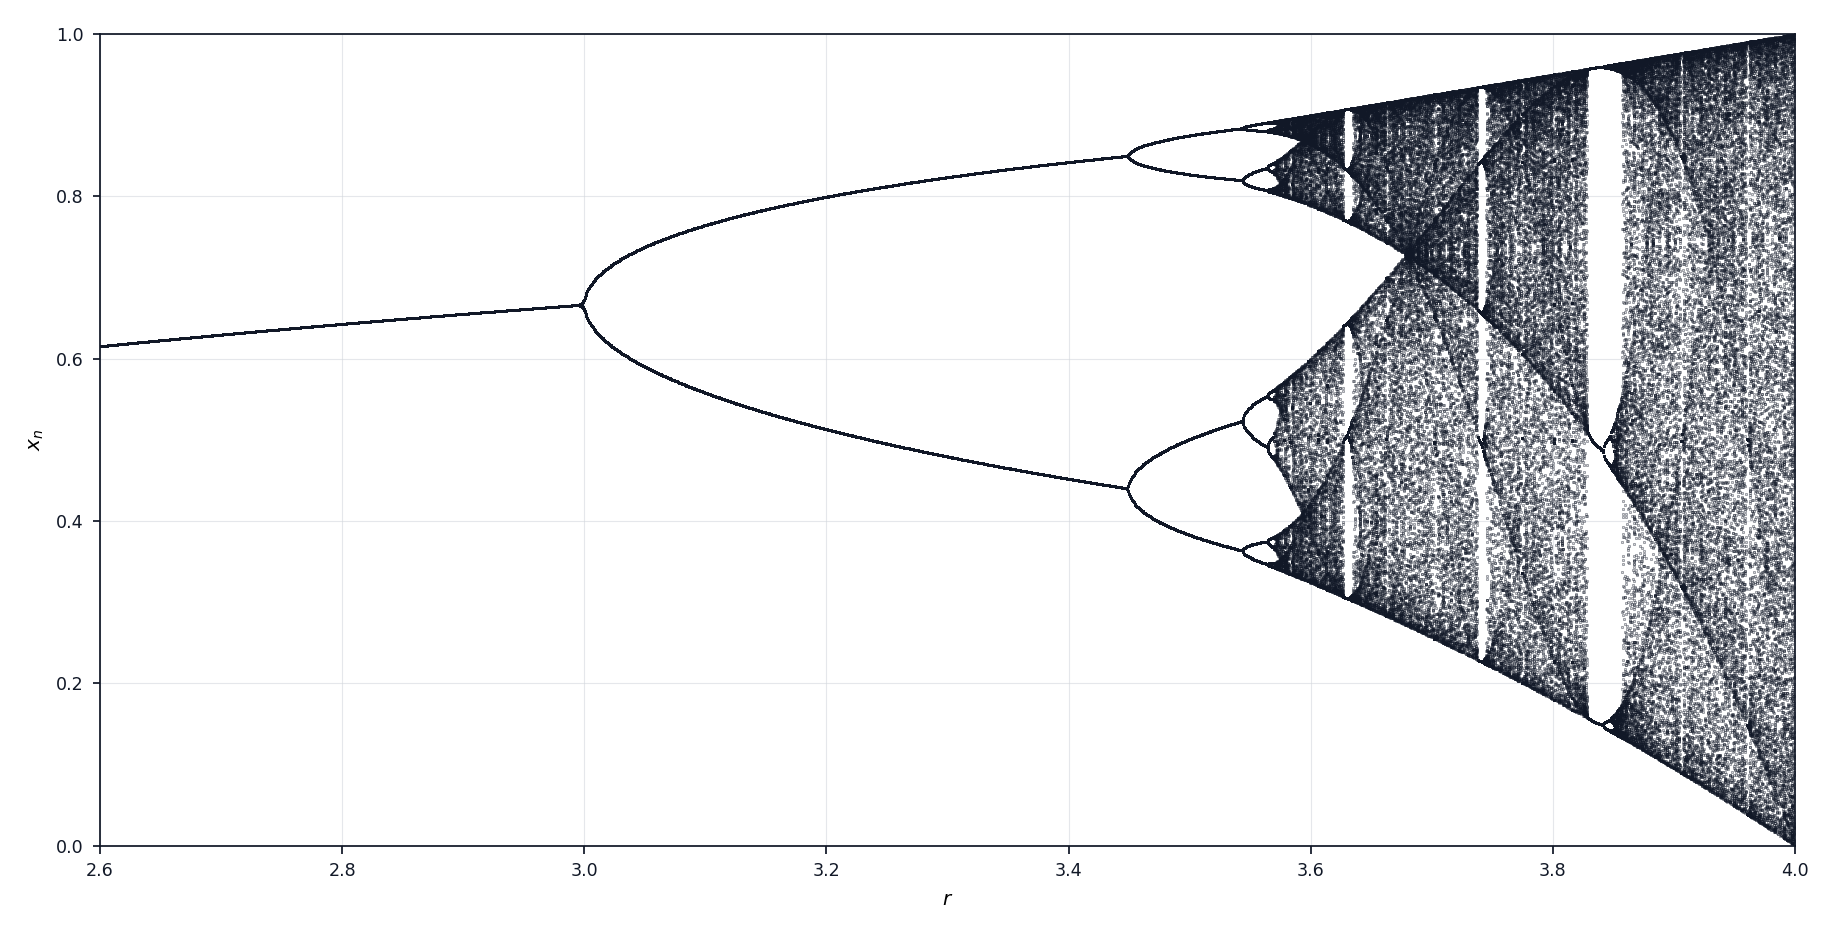
\includegraphics[width=\linewidth]{logistic_bifurcation.png}
\caption{Mapa logístico: valores tardíos por parámetro.}
\end{subfigure}\hfill
\begin{subfigure}[t]{0.49\textwidth}
\centering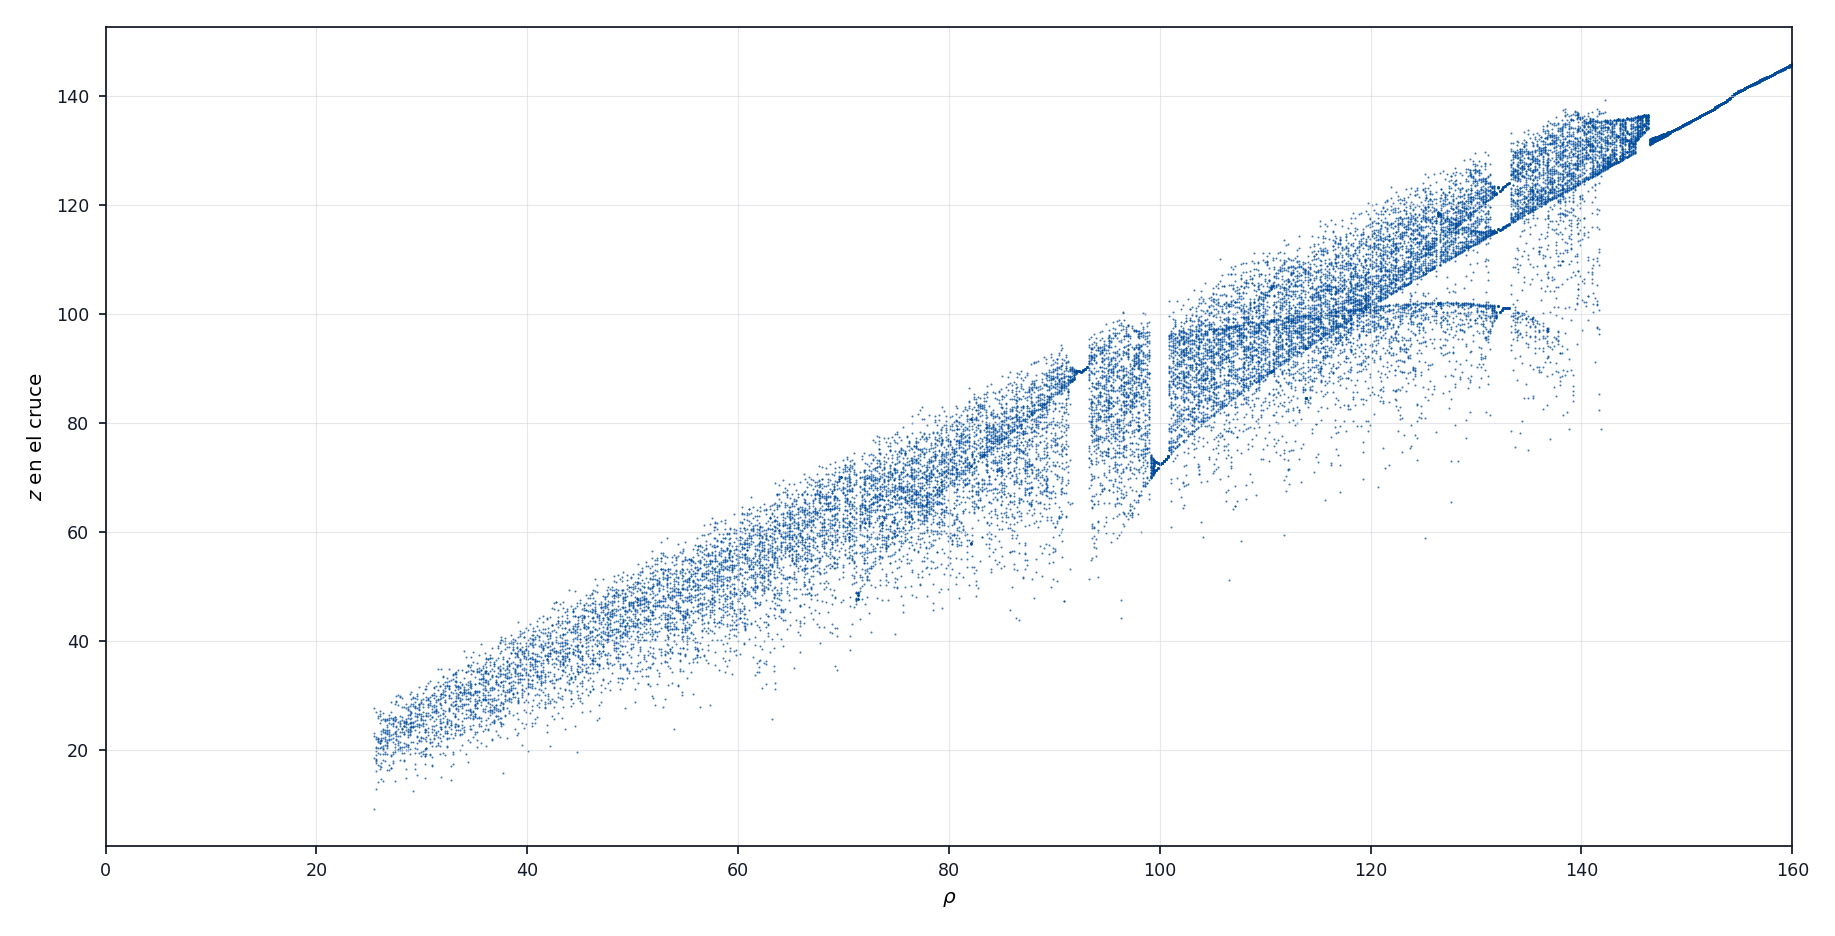
\includegraphics[width=\linewidth]{lorenz_bifurcation_rho.png}
\caption{Flujo de Lorenz: eventos de Poincaré o máximos.}
\end{subfigure}
\caption{Dos diagramas de bifurcación pueden parecer similares, aunque la observable
representada y el mecanismo de muestreo sean distintos.}
\label{fig:bifurcations}
\end{figure}

El diagrama permite localizar numéricamente un intervalo de cambio y formular una
hipótesis sobre
el tipo de bifurcación. La estimación precisa de $\mu_*$ requiere una malla suficiente, transitorios adecuados y repeticiones que separen una rama de un transitorio. La histéresis requiere barridos en ambas direcciones.

Como prueba práctica, calcule un diagrama con 200 valores y después refine sólo un
intervalo de interés.
Repita con el doble de transitorio y compare continuación contra reinicio independiente.
Marque como ``estructura confirmada'', ``sensible'' o ``inconclusa'' cada rama visible.

\subsection{Cuencas de atracción y fronteras}

Una cuenca relaciona condición inicial y destino; su lectura distingue la
multestabilidad del caos y revela el efecto de la resolución y el horizonte sobre las
fronteras. Dos estados iniciales casi iguales pueden terminar en regímenes distintos.
Una cuenca
colorea el espacio inicial según el destino y se complementa con trayectorias para
representar su evolución. Las fronteras suaves permiten cierta tolerancia experimental; las fronteras finas o
fractales reducen la predictibilidad del estado final \cite{grebogi1983}.

Formalmente, la cuenca de un atractor $A_i$ es
\[
 \mathcal B(A_i)=\{\mathbf{x}_0:\dist(\Phi_t(\mathbf{x}_0),A_i)\to0\}.
\]
Existe multestabilidad cuando, para los mismos parámetros, coexisten dos o más
atractores con cuencas no vacías. Una frontera de cuenca separa destinos. Su
estructura puede cuantificarse mediante exponentes de incertidumbre, medidas de
extensión o entropía de cuenca \cite{sprottxiong2015,daza2016}.

En una malla finita, el software implementa una clasificación operacional. Para cada
condición inicial detecta escape, convergencia a un equilibrio, periodicidad simple o
la clase acotada residual/no clasificada. Cambiar $T$, tolerancias o resolución
puede cambiar la etiqueta.

Para calcularla en Toolbox Chaos, en \gui{Cuenca de atracción} defina el rectángulo de
$(x_0,y_0)$, el valor fijo
$z_0$, $(N_x,N_y)$, $dt$ y tiempo total. Active \gui{Superponer equilibrios} para
relacionar geometría inicial y puntos fijos. Empiece con una malla pequeña y aumente
primero el horizonte si hay muchas celdas residuales; luego refine espacialmente.

En una sección bidimensional de Lorenz, por ejemplo, los colores representan destinos
detectados y categorías operativas de clasificación. Una región residual puede contener un transitorio largo,
una órbita periódica pendiente de clasificación o dinámica irregular. Las trayectorias de puntos
seleccionados ayudan a auditar la leyenda.

\begin{figure}[H]
\centering
\begin{subfigure}[t]{0.51\textwidth}
\centering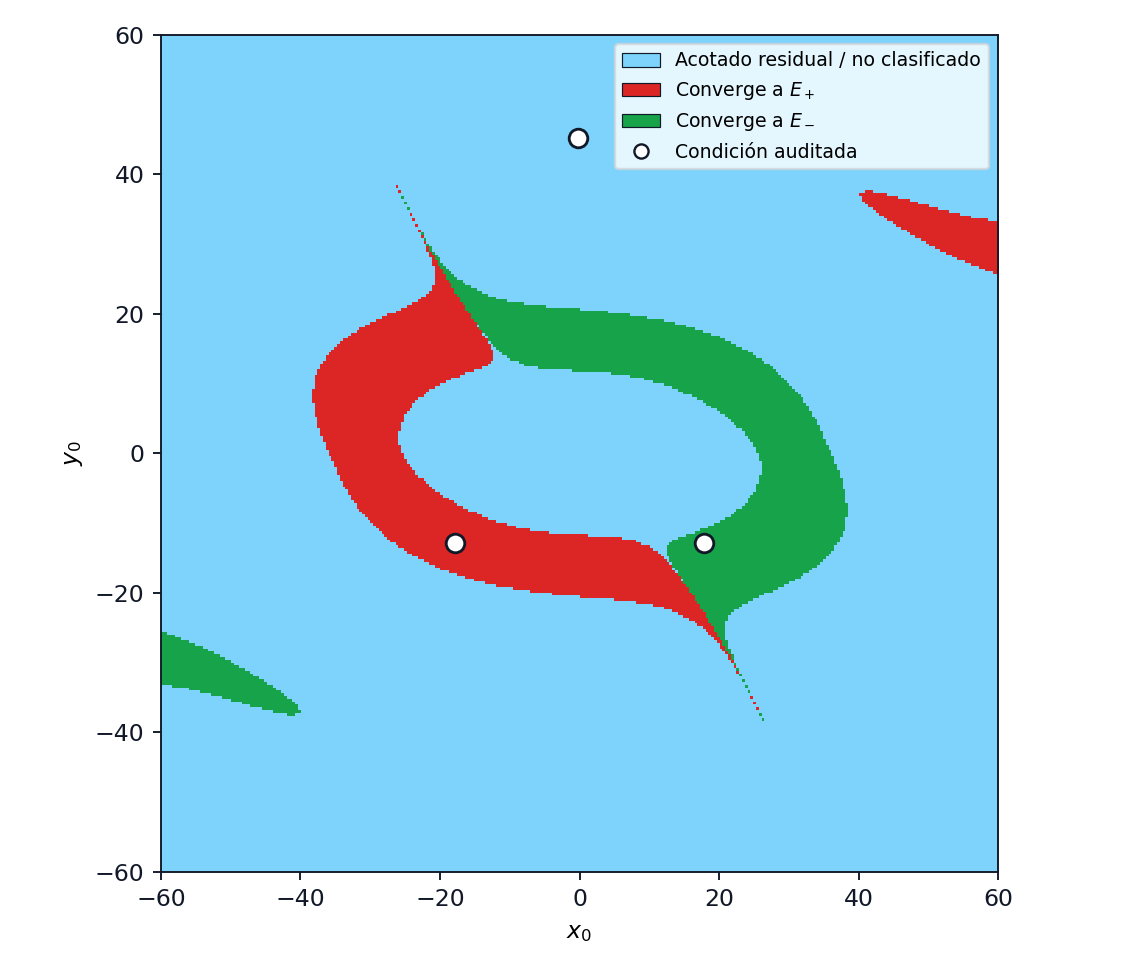
\includegraphics[width=\linewidth]{lorenz_basin_reading_zones.png}
\caption{Zonas de lectura y frontera en una sección de cuenca.}
\end{subfigure}\hfill
\begin{subfigure}[t]{0.36\textwidth}
\centering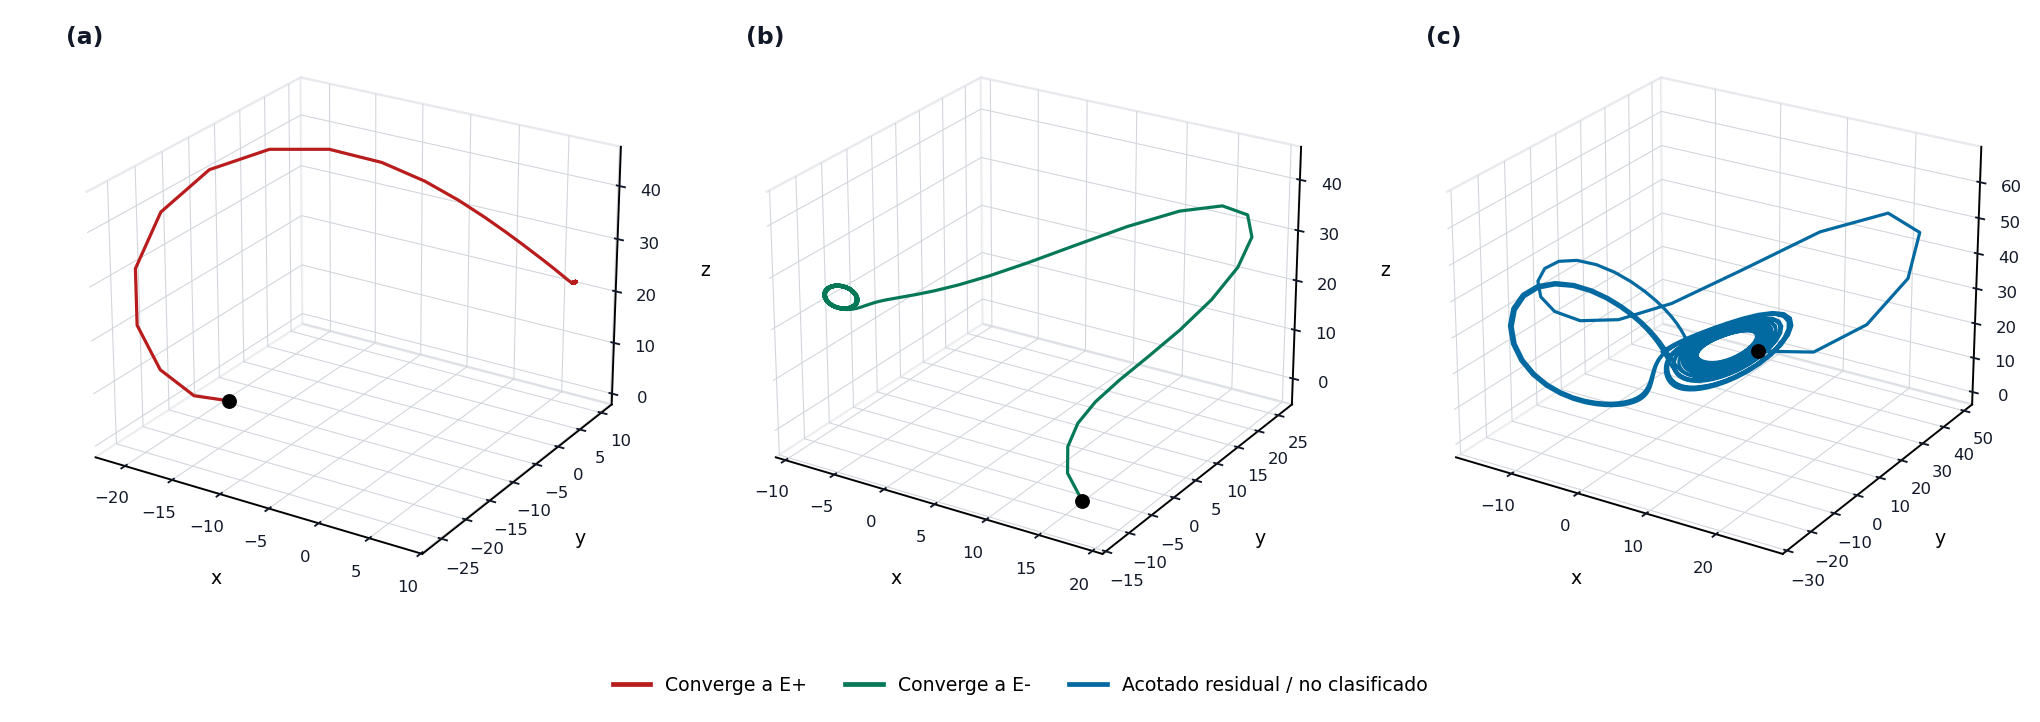
\includegraphics[width=\linewidth]{lorenz_basin_trajectories.png}
\caption{Trayectorias que auditan destinos coloreados.}
\end{subfigure}
\caption{La cuenca y las órbitas responden preguntas complementarias: ``desde dónde''
y ``hacia dónde/cómo''.}
\label{fig:basins}
\end{figure}

\begin{warningbox}
La coexistencia visual sólo muestra que las condiciones iniciales ensayadas alcanzaron
destinos distintos bajo el mismo conjunto de parámetros. La geometría global de las
cuencas y la naturaleza de su frontera requieren muestreo dirigido, control de
transitorios, refinamiento espacial y un argumento acorde con la propiedad estudiada.
\end{warningbox}

Con estas precauciones puede afirmarse coexistencia numérica de destinos para las
condiciones y el contrato
ensayados, y estimar fracciones de área de la sección. La descripción de toda la cuenca $n$-dimensional y de su fractalidad requiere análisis de escala y muestreo adicional a una sección 2D.

\begin{activitybox}{Refinamiento de cuencas y fronteras de clasificación}
Calcule una cuenca en $60\times60$ y $120\times120$. Seleccione diez puntos a ambos
lados de una frontera y aumente el tiempo total. Registre cuántas etiquetas cambian.
Interprete ese cambio como incertidumbre numérica antes de atribuirlo a fractalidad.
\end{activitybox}

\section{Lyapunov, análisis espectral y recurrencia}
\lecturaseccion{Robert C. Hilborn, \emph{Chaos and Nonlinear Dynamics: An Introduction for Scientists and Engineers}, capítulos 9--10 y apéndice A; Kathleen T. Alligood, Tim D. Sauer y James A. Yorke, \emph{Chaos: An Introduction to Dynamical Systems}, secciones 3.1--3.5, 4.5--4.7 y 5.2.}

El espectro de Lyapunov describe tasas medias de expansión y contracción, pero su signo
sólo se vuelve evidencia cuando la estimación muestra convergencia temporal. Para
formar una imagen geométrica, imagine una esfera diminuta de condiciones iniciales:
la dinámica la deforma en un
elipsoide: algunos ejes crecen, otros decrecen. Los exponentes de Lyapunov son las
tasas logarítmicas promedio de esos ejes.

Para una perturbación tangente, esta idea se expresa como
\[
 \lambda(\mathbf{x}_0,\mathbf v)=
 \limsup_{t\to\infty}\frac{1}{t}
 \log\frac{\|D\Phi_t(\mathbf{x}_0)\mathbf v\|}{\|\mathbf v\|}.
\]
El espectro ordenado $\lambda_1\ge\cdots\ge\lambda_n$ resume direcciones. En un
flujo autónomo típico, un exponente asociado a la dirección del flujo es cero. Un
máximo positivo es evidencia fuerte de sensibilidad promedio, bajo un cálculo
convergente y en el régimen correcto.

El algoritmo de Benettin integra el sistema variacional
\[
 \dot Y=J(\mathbf{x}(t))Y
\]
y aplica factorizaciones $Y=QR$ periódicas. Las sumas de
$\log|R_{ii}|$ evitan que todas las direcciones colapsen sobre la más expansiva
\cite{benettin1980a,benettin1980b}.

El cálculo se configura en \gui{Lyapunov} mediante $dt$, tiempo de quemado, tiempo
final y
\gui{QR cada N pasos}; después pulse \gui{Calcular exponentes de Lyapunov}. La vista
de convergencia es tan importante como los valores finales. La implementación visible
usa RK4 fijo para estado y sistema variacional en flujos ODE tridimensionales.

Para Lorenz clásico, por ejemplo, se espera un patrón aproximado $(+,0,-)$. La
primera curva cruce cero al inicio: debe estabilizarse al aumentar el horizonte. La
suma de exponentes puede contrastarse con la contracción promedio del volumen, pero
la igualdad exacta depende de hipótesis y del error numérico.

\begin{figure}[H]
\centering
\begin{subfigure}[t]{0.48\textwidth}
\centering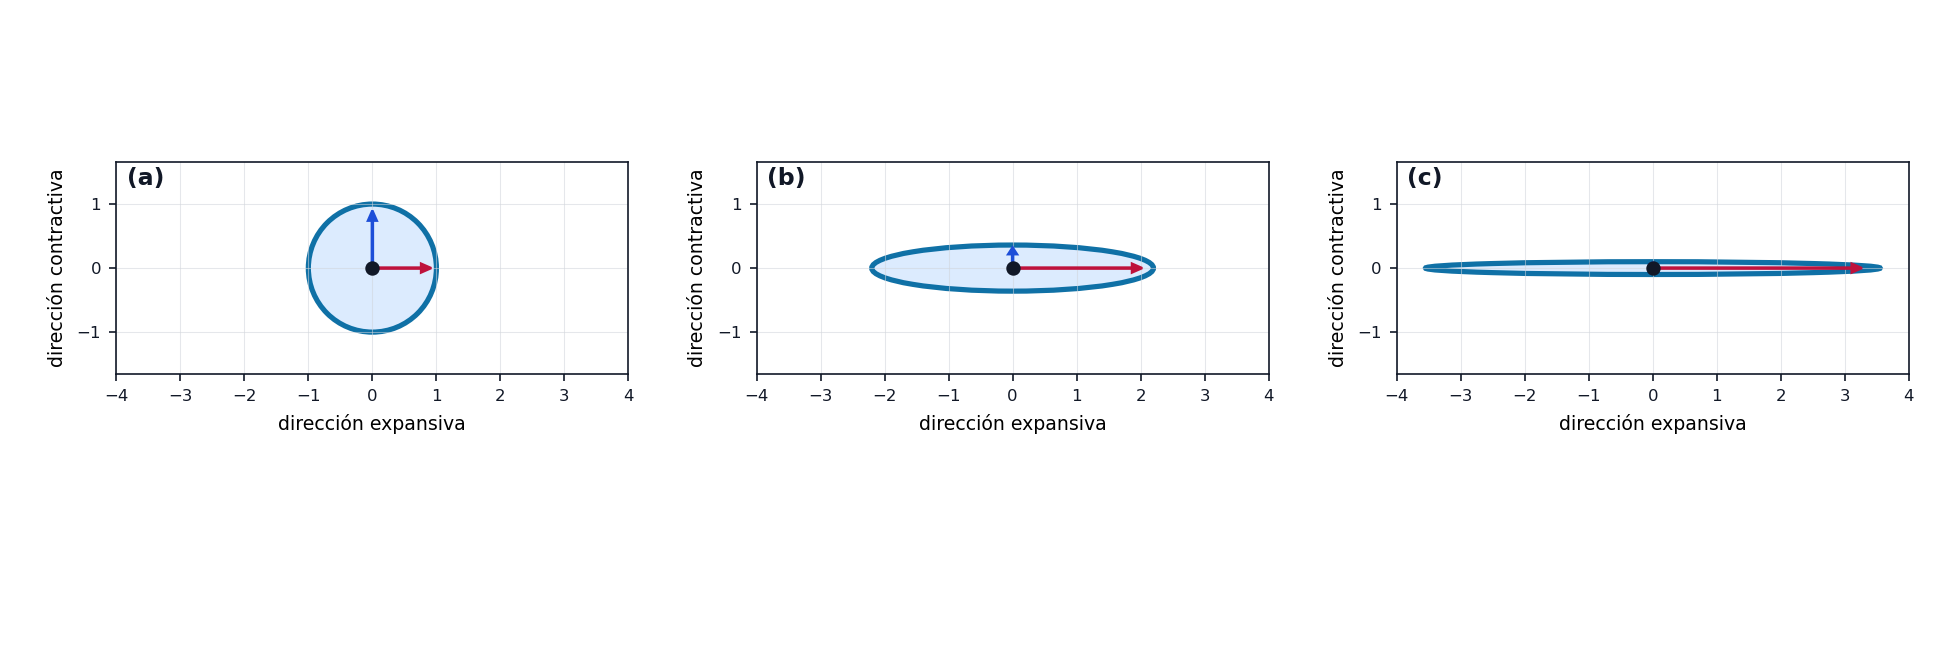
\includegraphics[width=\linewidth]{lyapunov_perturbation_concept.png}
\caption{Separación local de perturbaciones.}
\end{subfigure}\hfill
\begin{subfigure}[t]{0.48\textwidth}
\centering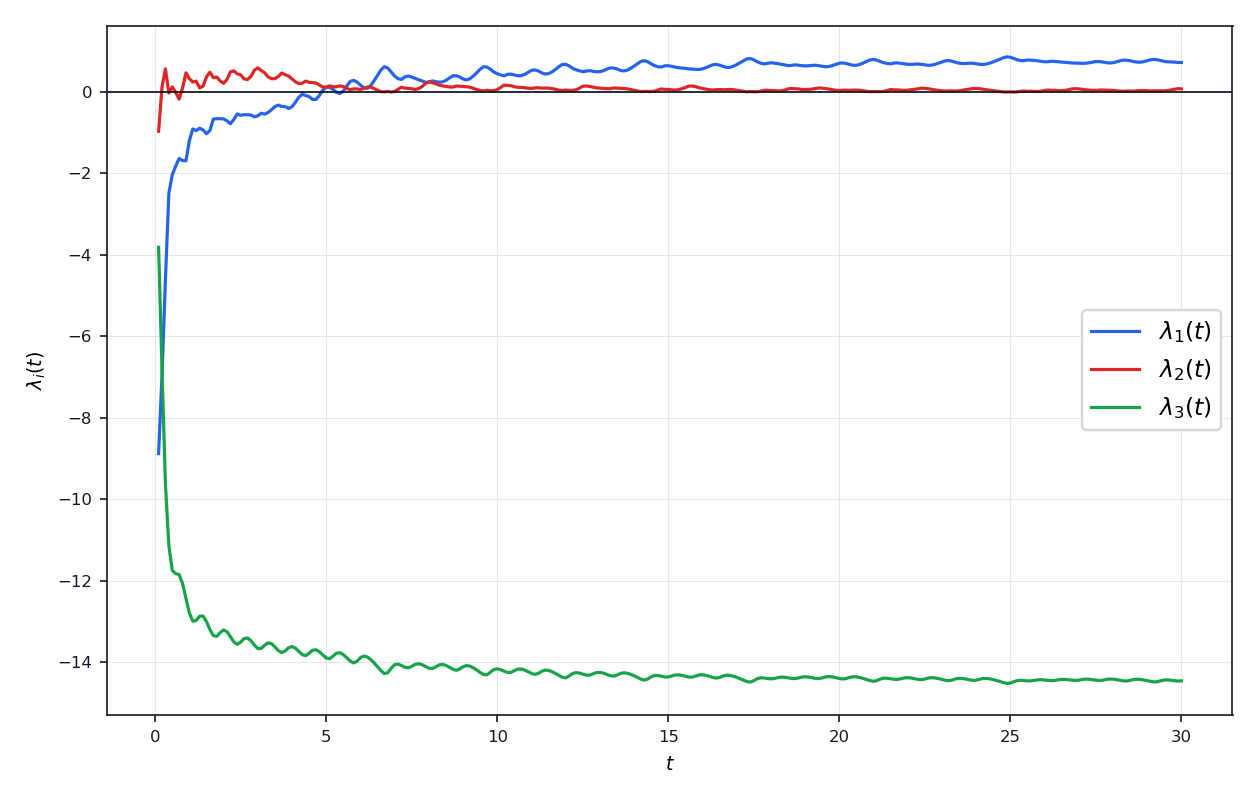
\includegraphics[width=\linewidth]{lorenz_lyapunov.png}
\caption{Estimaciones finitas y su convergencia.}
\end{subfigure}
\caption{El concepto geométrico y la estimación temporal deben leerse juntos.}
\label{fig:lyapunov}
\end{figure}

Sólo entonces puede reportarse un espectro finito que se estabiliza dentro de
tolerancias y es
estable frente a $dt$, tiempo y frecuencia QR. El límite asintótico requiere varios horizontes de integración, y un máximo positivo durante el transitorio se contrasta con la dinámica posterior antes de caracterizar un atractor caótico.

\begin{activitybox}{Convergencia del espectro de Lyapunov}
Calcule $\lambda_i(t)$ con dos tiempos finales y dos pasos. Construya una tabla con
el valor al final y la oscilación en el último 20\% del intervalo. Proponga una cifra
significativa justificada; cuando las curvas carecen de una meseta, reporte el estado
``no convergente'' y documente el patrón observado.
\end{activitybox}

\subsection{Espectro de amplitud y PSD de Welch}

El análisis frecuencial complementa esa lectura al relacionar periodicidad y contenido
en frecuencia, distinguir amplitud de densidad de potencia y evaluar una banda
ancha con diagnósticos de caos adicionales. Una serie temporal puede verse como suma de
oscilaciones. La transformada de Fourier
reorganiza la información por frecuencia. Una señal periódica ideal concentra energía
en líneas; una señal irregular reparte energía, pero el ruido, el transitorio y una
ventana corta también ensanchan el espectro.

Para muestras $x_n=x(n\Delta t)$, la transformada discreta es
\[
 X_k=\sum_{n=0}^{N-1}x_n e^{-2\pi i kn/N},\qquad
 f_k=\frac{k}{N\Delta t}.
\]
La resolución aproximada es $\Delta f=1/(N\Delta t)$ y la frecuencia de Nyquist es
$f_N=1/(2\Delta t)$. Restar la media y usar una ventana reduce fuga espectral, pero
modifica amplitudes y anchuras.

Welch divide la señal en segmentos superpuestos, calcula periodogramas modificados y
los promedia. Reduce varianza a cambio de resolución frecuencial \cite{welch1967}.
La PSD tiene unidades de la variable al cuadrado por unidad de frecuencia; el espectro
de amplitud conserva otra normalización y responde una pregunta diferente.

En la pestaña \gui{Espectro}, elija \gui{PSD de Welch (recomendado)} o
\gui{Espectro de amplitud}, defina el transitorio y, si es necesario, límites de
frecuencia. Pulse \gui{Calcular FFT/PSD}. Use \gui{Usar última trayectoria} para que
las tres variables provengan exactamente del mismo cálculo.

En Lorenz, $x(t)$, $y(t)$ y $z(t)$ presentan espectros propios porque observan la
misma dinámica mediante coordenadas distintas. Una frecuencia dominante puede
reflejar el tiempo medio de giro de un lóbulo dentro de una señal irregular.

\begin{figure}[H]
\centering
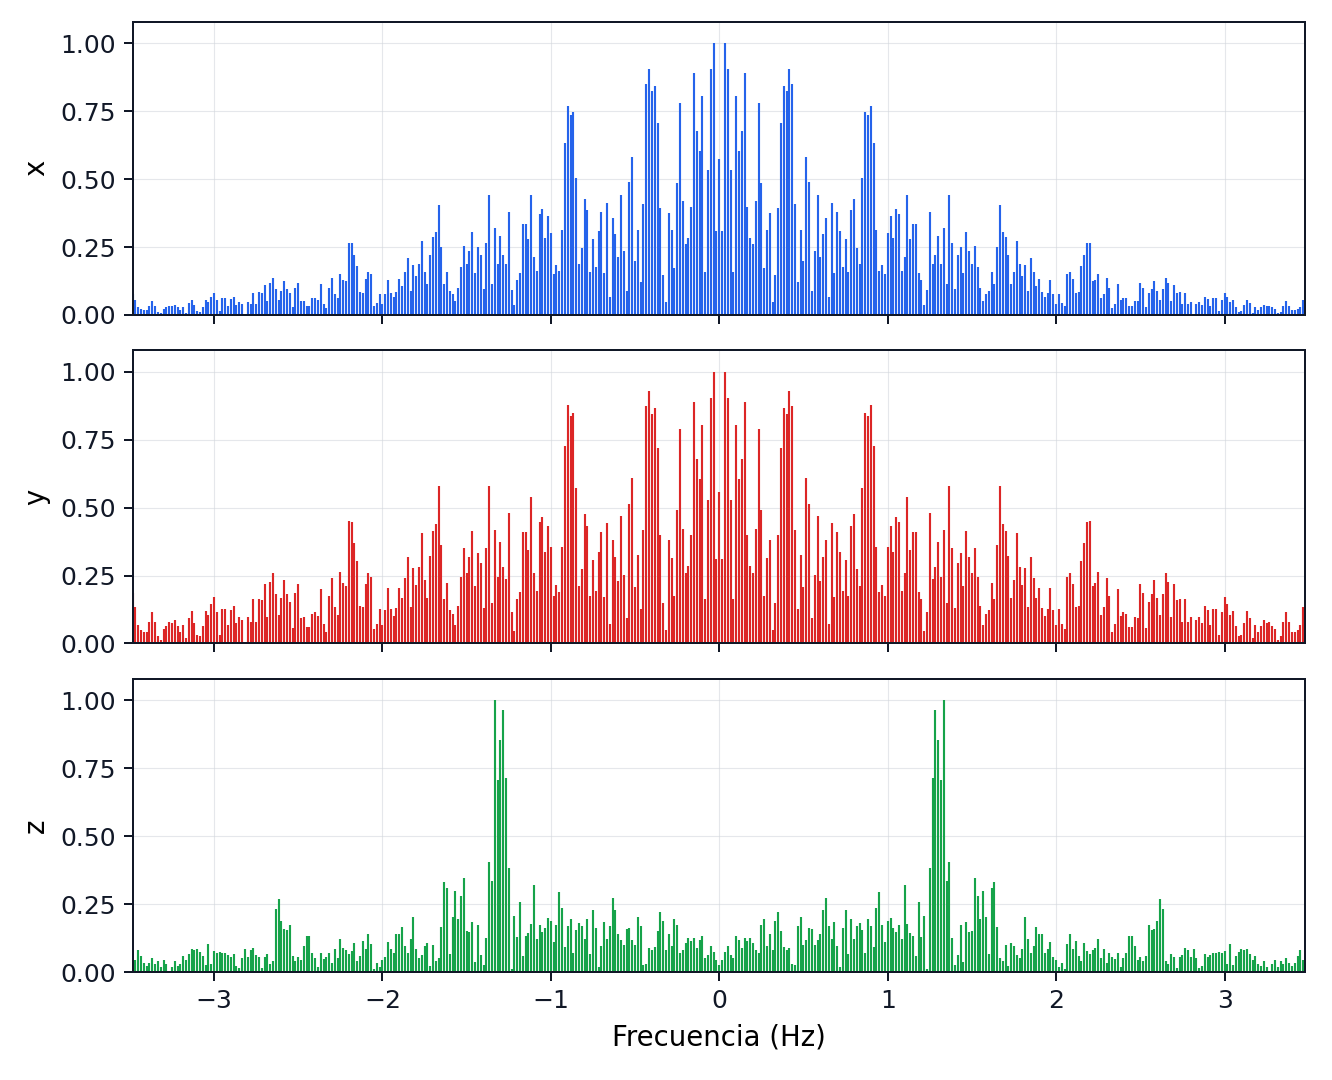
\includegraphics[width=0.70\textwidth]{lorenz_fft.png}
\caption{Espectro normalizado centrado para las variables de Lorenz. La comparación entre
componentes debe conservar el mismo paso, horizonte y transitorio.}
\label{fig:fft}
\end{figure}

El espectro permite localizar periodicidad dominante, armónicos y distribución
frecuencial bajo
el muestreo elegido. La distinción entre caos determinista y ruido requiere diagnósticos adicionales a una banda ancha; la identificación de un ciclo límite exige más evidencia que un pico espectral.

Como comprobación, compare una órbita periódica y Lorenz con igual $\Delta t$ y
duración útil. Repita
Welch con segmentos más cortos y más largos. Anote qué gana en suavidad y qué pierde
en resolución. Verifique que ningún pico interpretado esté por encima de Nyquist.

\subsection{Secciones de Poincaré, dimensión de correlación y recurrencia}

Tres herramientas adicionales resumen geometría y repetición: la sección de Poincaré,
la dimensión de correlación y la matriz de recurrencia. Una trayectoria larga puede
ser difícil de leer. Una sección registra sólo cruces; la
dimensión pregunta cómo crece el número de pares cercanos al cambiar la escala; la
recurrencia marca cuándo el sistema vuelve cerca de un estado previo. Las tres
herramientas comprimen información, pero cada una puede crear artefactos si se eligen
mal el umbral o la escala.

Una sección de Poincaré $\Sigma$ registra intersecciones transversales de la órbita.
Un ciclo límite produce un punto fijo del mapa de retorno; dinámicas más complejas
producen conjuntos de cruces.

Para $N$ estados, la suma de correlación
\[
 C(r)=\frac{2}{N(N-1)}\sum_{i<j}
 \mathbf 1\bigl(\|\mathbf{x}_i-\mathbf{x}_j\|<r\bigr)
\]
puede obedecer $C(r)\propto r^{D_2}$ en una región de escala, y entonces
\[
 D_2\approx\frac{\dd\log C(r)}{\dd\log r}.
\]
La estimación de Grassberger--Procaccia requiere una meseta de pendiente y suficientes
datos; la validación selecciona una meseta de pendiente y documenta su intervalo \cite{grassberger1983}.

Una matriz de recurrencia se define por
\[
 R_{ij}=\mathbf 1\bigl(\|\mathbf{x}_i-\mathbf{x}_j\|\le\varepsilon\bigr).
\]
Sus diagonales y bloques muestran retornos y cambios de régimen, con fuerte
dependencia del umbral y del muestreo \cite{eckmann1987}.

En la GUI actual, \gui{Bifurcación} puede construir eventos de Poincaré o máximos en
flujos compatibles. La dimensión de correlación y las matrices de recurrencia se
se presentan aquí como una ampliación teórica externa: estos cálculos se realizan con
una serie de estados obtenida o generada fuera de estas pestañas. Para aplicarlos, el
equipo investigador documenta por separado el procedimiento empleado y verifica la
ruta de exportación en la versión instalada.

La figura siguiente corta Lorenz con un plano. Los puntos corresponden a eventos de
una misma órbita. Un plano transversal representa el retorno con precisión y exige
indicar su orientación y sentido de cruce.

\begin{figure}[H]
\centering
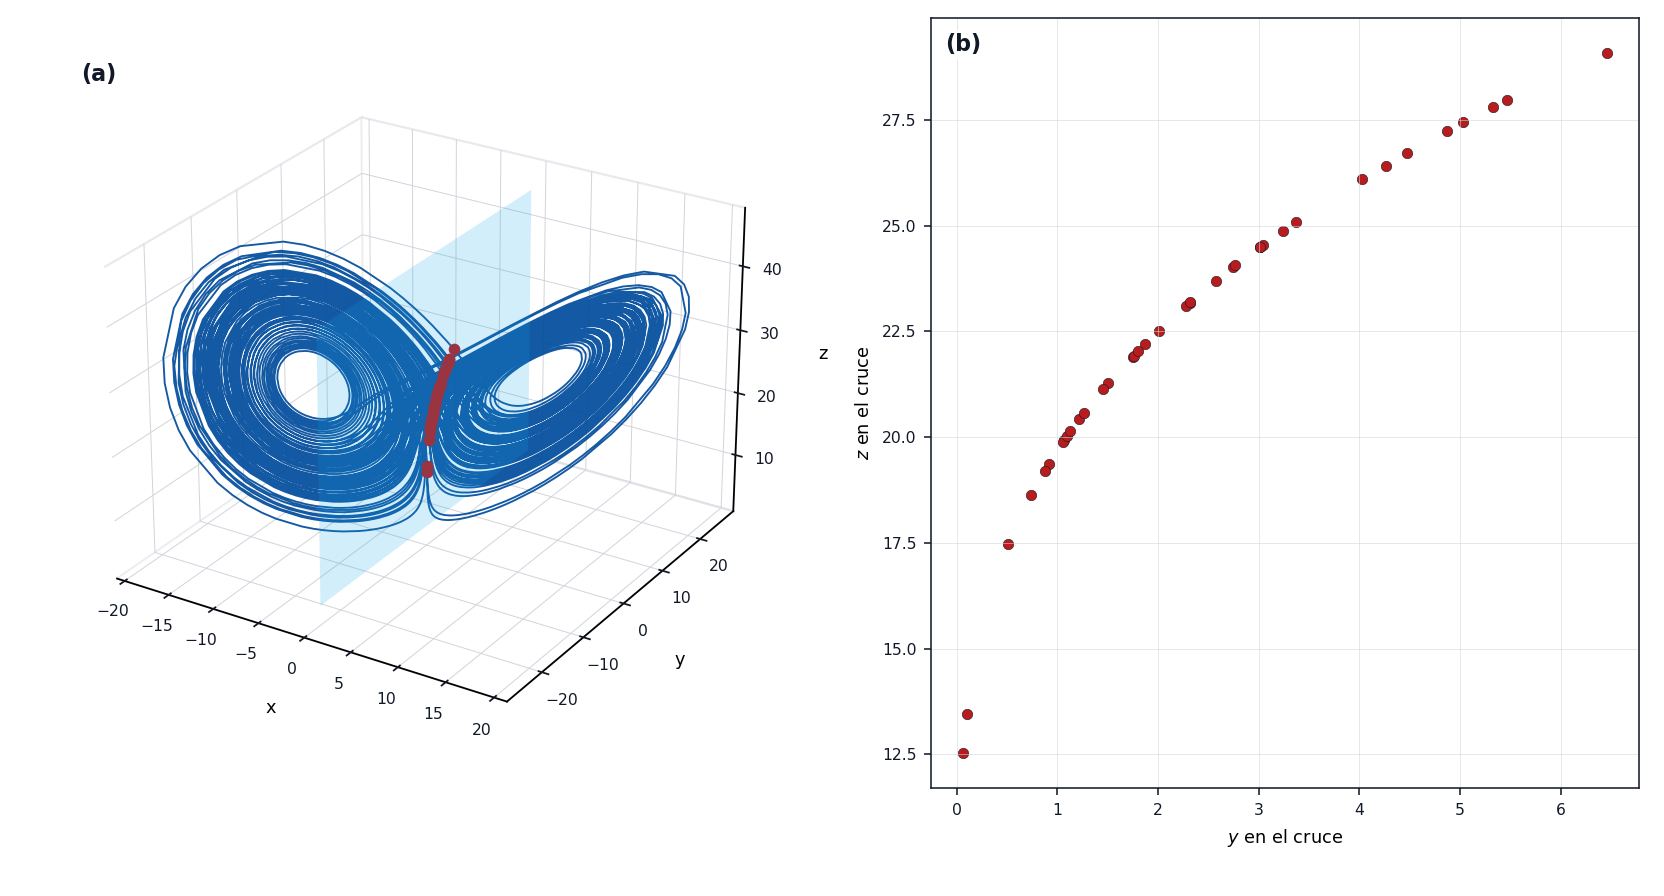
\includegraphics[width=0.62\textwidth]{lorenz_poincare_section.png}
\caption{Sección de Poincaré producida a partir de una trayectoria de Lorenz.}
\label{fig:poincare}
\end{figure}

Con datos externos adecuadamente documentados puede estimarse una ley de escala en un
intervalo explícito o describirse recurrencia
para un umbral declarado. La dimensión fractal requiere varios ajustes y las matrices comparadas deben usar normalizaciones compatibles. Las series cortas, sobremuestreadas o ruidosas exigen controles de sesgo.

Como ampliación, construya una sección usando dos planos diferentes y compare el
número y distribución
de cruces. Para dimensión, grafique $\log C(r)$ contra $\log r$ y marque regiones
dominadas por saturación y escasez de pares. Una meseta estable sustenta la estimación;
su ausencia se documenta como evidencia adicional requerida.

\section{Sistemas fraccionarios y criterio de Matignon}
\lecturaseccion{Como contexto de estabilidad y linealización, Morris W. Hirsch, Stephen Smale y Robert L. Devaney, \emph{Differential Equations, Dynamical Systems, and an Introduction to Chaos}, capítulos 7--10; para el operador y el criterio fraccionario, véanse las referencias primarias de Caputo y Matignon al final del manual.}

La derivada de Caputo introduce memoria y el criterio angular de Matignon caracteriza
una clase de sistemas lineales de orden común; ambos conceptos requieren una adaptación
explícita de los diagnósticos de orden entero. En una ecuación ordinaria, la
derivada local resume el cambio inmediato. En una
ecuación fraccionaria, el estado actual depende de una historia ponderada. El orden
$q$ modifica el modelo y la noción de estado necesaria para predecir el futuro; su
papel corresponde a una memoria ponderada, distinta del ajuste del paso numérico.

Para $0<q<1$, la derivada de Caputo puede escribirse
\[
 {}^{C}D_t^q x(t)=\frac{1}{\Gamma(1-q)}
 \int_0^t\frac{x'(\tau)}{(t-\tau)^q}\dd\tau .
\]
El núcleo $(t-\tau)^{-q}$ conserva memoria de toda la historia. En el límite
$q\to1$ se recupera la derivada ordinaria bajo condiciones apropiadas. La forma de
Caputo facilita condiciones iniciales expresadas con valores ordinarios
\cite{caputo1967}.

Para el sistema lineal conmensurable
\[
 {}^{C}D_t^q\mathbf{x}=A\mathbf{x},\qquad 0<q<1,
\]
el criterio de Matignon establece estabilidad asintótica si y sólo si
\[
 |\arg(\lambda_i)|>\frac{q\pi}{2}
 \quad\text{para todo }\lambda_i\in\sigma(A)
\]
en el caso considerado \cite{matignon1996}. Para $q=1$ la frontera corresponde al
eje imaginario. Para $q=0.5$, el sector excluido alrededor del eje real positivo
tiene semiancho $\pi/4$: el criterio se evalúa mediante el argumento de cada
autovalor.

El plano de \gui{Autovalores} ayuda a ubicar $\lambda_i$, pero la interpretación por
semiplanos es la de orden entero. Para un cálculo fraccionario debe declararse el
operador, orden común o no común, historia, método y criterio aplicable. Las funciones
fraccionarias del núcleo matemático pueden utilizarse desde código cuando estén
expuestas por la versión instalada; cada diagnóstico tangente entero requiere confirmar su extensión hereditaria validada.

Para ver la diferencia, considere un autovalor $\lambda=1+2i$, cuyo argumento es
aproximadamente $63.4^\circ$.
Para $q=1$, su parte real positiva lo hace inestable. Para $q=0.5$, el umbral de
Matignon es $45^\circ$, de modo que satisface el criterio angular del sistema lineal
conmensurable. Este contraste exige usar la frontera angular correspondiente al plano fraccionario. El ejemplo es exclusivamente lineal y local:
clasifica la estabilidad de la linealización bajo las hipótesis de Matignon; la
estabilidad global del sistema no lineal y la existencia de un atractor requieren
evidencia adicional.

\begin{evidencebox}{Contrato mínimo para un resultado fraccionario}
Reporte: definición de derivada, orden u órdenes, condición/historia inicial, método
de convolución o integración, paso, horizonte, tratamiento de memoria, tolerancias y
prueba de refinamiento. Dos métodos con nombres parecidos pueden discretizar
operadores diferentes.
\end{evidencebox}

En consecuencia, puede aplicarse el criterio de Matignon a la linealización
conmensurable bajo sus
hipótesis. Su aplicación requiere adaptación para órdenes no conmensurables, sistemas no
lineales globales o aproximaciones que cambian el operador. Una trayectoria
fraccionaria aparentemente caótica requiere diagnósticos específicos de caos y estabilidad global.

\begin{activitybox}{Criterio de Matignon para distintos órdenes fraccionarios}
Dibuje los rayos $\arg\lambda=\pm q\pi/2$ para $q=1$, $0.8$ y $0.5$. Clasifique
los autovalores $1+2i$, $-1+i$ y $2+0.5i$. Después explique por qué disminuir
$q$ cambia la región estable con la matriz $A$ fija.
\end{activitybox}

% Geometría, topología y memoria. Se incluye desde manual_teorico_pedagogico.tex.

\section{Geometría, topología y memoria en sistemas dinámicos}
\label{sec:geometria-topologia-memoria}

\begin{objectivebox}
Construir una lectura universitaria del sistema dinámico como objeto geométrico:
identificar el espacio donde vive, pasar del problema de valor inicial al flujo,
reconocer invariancia y atracción, estudiar la deformación local de perturbaciones y
reducir órbitas periódicas a mapas de retorno. La última parte explica qué cambia
cuando la evolución conserva memoria mediante una derivada de Caputo y deriva el
esquema ABM--PECE desde la ecuación integral de Volterra.
\end{objectivebox}

Este capítulo reúne ideas que suelen estudiarse en cursos distintos. La topología
aporta el vocabulario de vecindad, frontera, continuidad y compacidad. La geometría
diferencial permite interpretar un campo como una dirección tangente en cada estado.
La teoría cualitativa de ecuaciones diferenciales organiza órbitas, conjuntos límite,
variedades invariantes y retornos. El análisis numérico convierte esas construcciones
en experimentos y conserva sus hipótesis explícitas. El propósito es aprender a moverse
entre esos cuatro niveles con sus funciones diferenciadas.

La secuencia de trabajo será siempre la misma. Primero se declara el espacio de
fases y el modelo; después se obtiene una propiedad analítica; luego se decide qué
gráfica puede hacerla visible; finalmente se delimita el alcance de la evidencia disponible.
Esta disciplina vincula cada figura con las conclusiones que su método sostiene.

\subsection{Topología del espacio de fases}

\paragraph{Abiertos, vecindades y continuidad.}
Una topología sobre un conjunto $X$ es una familia $\mathcal T$ de subconjuntos,
llamados abiertos, que contiene a $\varnothing$ y a $X$, es cerrada bajo uniones
arbitrarias y bajo intersecciones finitas. Una vecindad de $x$ es cualquier conjunto
que contiene un abierto al que pertenece $x$. Esta definición parece abstracta, pero
responde una pregunta concreta: ¿qué significa que dos estados sean próximos y que
una solución dependa continuamente de su condición inicial?

En $\R^n$ se usa normalmente la topología inducida por la distancia euclídea

\begin{equation}
 d_2(x,y)=\left(\sum_{j=1}^{n}|x_j-y_j|^2\right)^{1/2}.
 \label{eq:gt-metrica-euclidea}
\end{equation}

Una función $h:X\to Y$ es continua si la preimagen de todo abierto de $Y$ es abierta
en $X$. La formulación por preimágenes no depende de coordenadas particulares y por
eso resulta adecuada al comparar modelos escritos con variables distintas.

\paragraph{Interior, clausura y frontera.}
Para $A\subset X$, el interior $\operatorname{int}A$ reúne los puntos que poseen una
vecindad contenida en $A$; la clausura $\overline A$ añade todos sus puntos de
acumulación. La frontera es

\begin{equation}
 \partial A=\overline A\setminus\operatorname{int}A.
 \label{eq:gt-frontera}
\end{equation}

Toda vecindad de un punto de $\partial A$ encuentra puntos de $A$ y de su
complemento. Una frontera calculada sobre una malla sólo aproxima esta definición:
el último píxel de un color sólo registra una aproximación del conjunto matemático
$\partial A$.

\paragraph{Compacidad y conexidad.}
Un conjunto compacto de $\R^n$ es cerrado y acotado. Esta equivalencia no se
traslada automáticamente a espacios generales, pero en el curso será una herramienta
frecuente: permite extraer subsucesiones convergentes y evita que una órbita salga a
distancias arbitrarias dentro del conjunto considerado. Un conjunto conexo no puede
separarse en dos abiertos relativos, disjuntos y no vacíos. Compacidad controla la
posibilidad de tomar límites; conexidad controla la posibilidad de separar el objeto.

\paragraph{Producto y cociente.}
Algunos espacios de fases adoptan una geometría distinta de $\R^n$. En un péndulo, el ángulo satisface
$\theta\sim\theta+2\pi k$; por ello el estado natural es
$S^1\times\R$, no un rectángulo con dos bordes físicos diferentes. Una distancia
angular compatible es

\begin{equation}
 d_{S^1}(\theta_1,\theta_2)
 =\min_{k\in\mathbb Z}|\theta_1-\theta_2+2\pi k|.
 \label{eq:gt-distancia-circular}
\end{equation}

Si una curva cruza el borde derecho de una gráfica angular y reaparece en el
izquierdo, no ha saltado en el espacio de fases: la discontinuidad pertenece a la
carta usada para dibujarla. Esta distinción es decisiva al interpretar trayectorias,
retornos y distancias.

\begin{activitybox}{Práctica reproducible: una frontera exacta y su aproximación}
En \gui{Crear sistema} defina las variables \code{x,y,z}, sin parámetros, con
ecuaciones \code{x-x**3}, \code{-y} y \code{-z}. Use RK4,
$h=0.01$, $T=20$ y los estados iniciales
$(0.25,0.5,0.2)$, $(-0.25,0.5,0.2)$, $(0.01,0.5,0.2)$ y
$(-0.01,0.5,0.2)$. Guarde las series y los retratos con nombres que incluyan el
signo de $x_0$. Antes de simular, demuestre con una línea de fase que $x=0$ es la
frontera entre los destinos $x=1$ y $x=-1$. Después explique por qué cuatro
trayectorias ilustran esa conclusión, pero no la sustituyen.
\end{activitybox}

\paragraph{Lectura topológica de las gráficas.}
Una serie temporal informa cómo se recorre el estado; un retrato de fase informa qué
región se visita; una gráfica de condiciones iniciales informa qué destino se asignó
a cada punto. Ninguna vista contiene por sí sola las otras dos. Si una separación
parece brusca, hay que preguntar si procede de la dinámica, de la identificación de
coordenadas, de una tolerancia del clasificador o de la resolución elegida.

\begin{figure}[H]
\centering
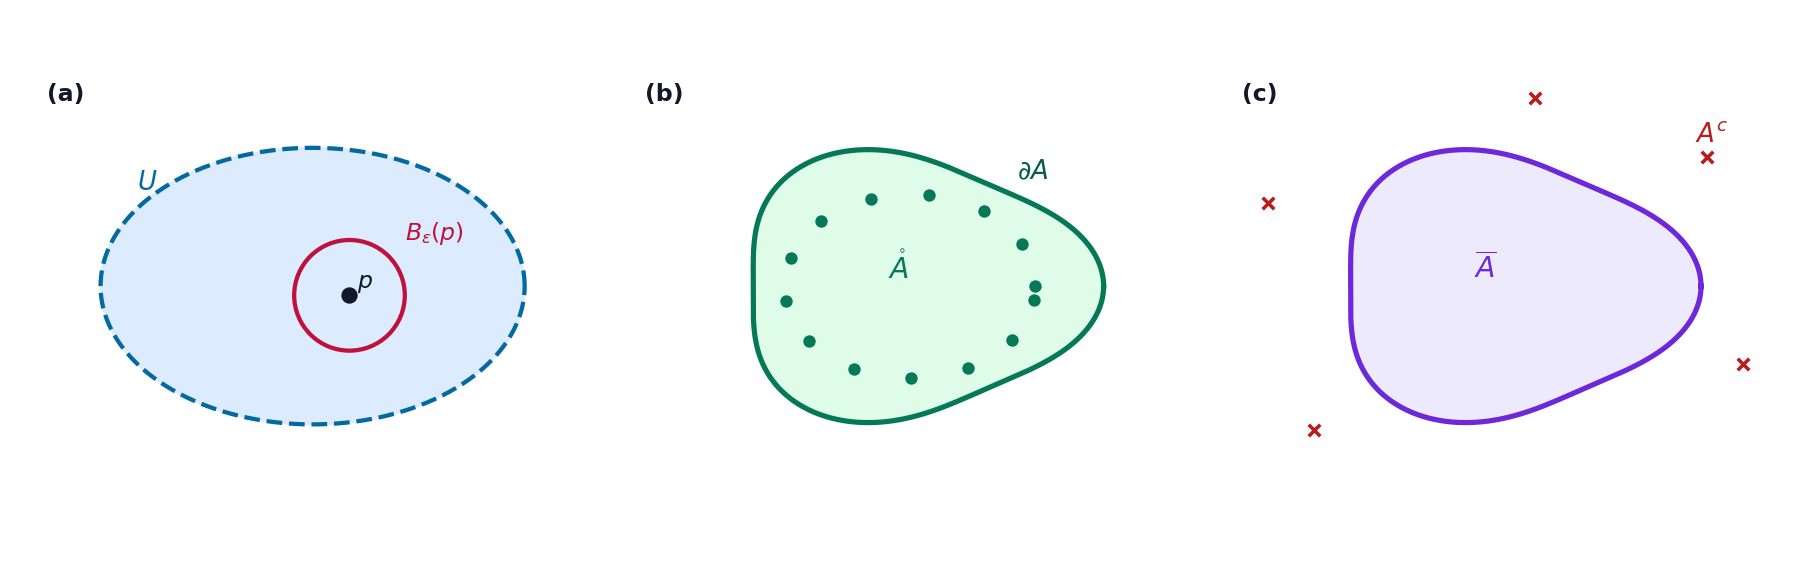
\includegraphics[width=0.92\linewidth]{topology_neighborhood_boundary.png}
\caption{Lectura mínima de un conjunto en el espacio de fases: (a) una vecindad
abierta alrededor de un punto, (b) interior y frontera, y (c) clausura frente al
complemento. El trazo de la frontera es información geométrica; la pertenencia y la
apertura son propiedades del conjunto y de la topología elegida.}
\label{fig:gt-topologia-minima}
\end{figure}

\lecturaseccion{Eduardo Nahmad-Achar, \emph{Topología y geometría diferencial con
aplicaciones a la física}, capítulos sobre espacios topológicos, variedades y campos;
Morris W. Hirsch, Stephen Smale y Robert L. Devaney, \emph{Differential Equations,
Dynamical Systems, and an Introduction to Chaos}, capítulos 1--3.}

\subsection{Problema de valor inicial y flujo}

Considérese una ecuación autónoma

\begin{equation}
 \dot x=f(x),\qquad x(0)=x_0,\qquad x\in U\subset\R^n.
 \label{eq:gt-pvi}
\end{equation}

Si $f$ es localmente Lipschitz, el teorema de Picard--Lindelöf proporciona una
solución local única. La palabra \emph{local} importa: un campo polinómico puede
tener solución sólo hasta un tiempo finito si no se dispone de una cota que impida
el crecimiento sin límite. Cuando la solución existe en el intervalo requerido se
define

\begin{equation}
 \Phi_t(x_0)=x(t;x_0).
 \label{eq:gt-flujo-def}
\end{equation}

La autonomía y la unicidad producen la ley de composición

\begin{equation}
 \Phi_0=\operatorname{id},\qquad
 \Phi_{t+s}=\Phi_t\circ\Phi_s.
 \label{eq:gt-ley-flujo}
\end{equation}

La derivación es breve. Las funciones $u(t)=\Phi_{t+s}(x_0)$ y
$v(t)=\Phi_t(\Phi_s(x_0))$ resuelven la misma ecuación y comparten el dato inicial
$u(0)=v(0)=\Phi_s(x_0)$. Por unicidad, coinciden. Si cada solución puede prolongarse
hacia tiempos positivos y negativos, $\Phi_t$ es un flujo; si sólo se dispone de
$t\geq0$, se habla de semiflujo.

\paragraph{Órbita e invariancia.}
La órbita de $x_0$ es el conjunto de estados visitados,

\begin{equation}
 \mathcal O(x_0)=\{\Phi_t(x_0):t\in I_{x_0}\}.
 \label{eq:gt-orbita}
\end{equation}

Un conjunto $A$ es positivamente invariante si $\Phi_t(A)\subseteq A$ para todo
$t\geq0$. Es invariante si la igualdad se conserva para todo tiempo admisible. La
invariancia es una afirmación sobre todas las trayectorias que comienzan en $A$, no
una impresión obtenida de una curva dibujada dentro de él.

Para una región $N=\{x:h(x)\leq0\}$ con frontera regular, el signo de la derivada de
Lie

\begin{equation}
 L_fh(x)=\nabla h(x)^{\mathsf T}f(x)
 \label{eq:gt-derivada-lie}
\end{equation}

indica si el campo entra o sale. Si $L_fh<0$ en $\partial N$, el campo apunta
estrictamente hacia el interior y $N$ es positivamente invariante. Una integral
promedio negativa sobre la frontera requiere controlar el signo punto
por punto o usar un argumento global distinto.

\paragraph{Ejemplo resuelto: contracción anisótropa.}
Para

\begin{equation}
 \dot x=-x,\qquad \dot y=-2y,
 \label{eq:gt-lineal-contractivo}
\end{equation}

la solución es

\begin{equation}
 \Phi_t(x_0,y_0)=(e^{-t}x_0,e^{-2t}y_0).
 \label{eq:gt-flujo-contractivo}
\end{equation}

Cada eje y cada cuadrante cerrado son positivamente invariantes. Las órbitas se
aproximan al origen, pero no lo hacen a la misma velocidad: la componente $y$ pierde
una fracción fija más rápido. En un retrato de fase se obtiene
$y=Cx^2$ dentro de cada región de signo constante. La geometría de la curva elimina
el tiempo; la serie temporal conserva las tasas.

\begin{activitybox}{Ejercicio con pista: flujo e invariancia}
Para \eqref{eq:gt-lineal-contractivo}, compruebe directamente
\eqref{eq:gt-ley-flujo}. Después use
$V(x,y)=x^2+y^2$ y calcule $\dot V$. ¿Qué discos son positivamente invariantes?
\textbf{Pista:} $\dot V=-2x^2-4y^2$; compare el signo en cada circunferencia y no
confunda invariancia del disco con invariancia de cada circunferencia.
\end{activitybox}

\begin{figure}[H]
\centering
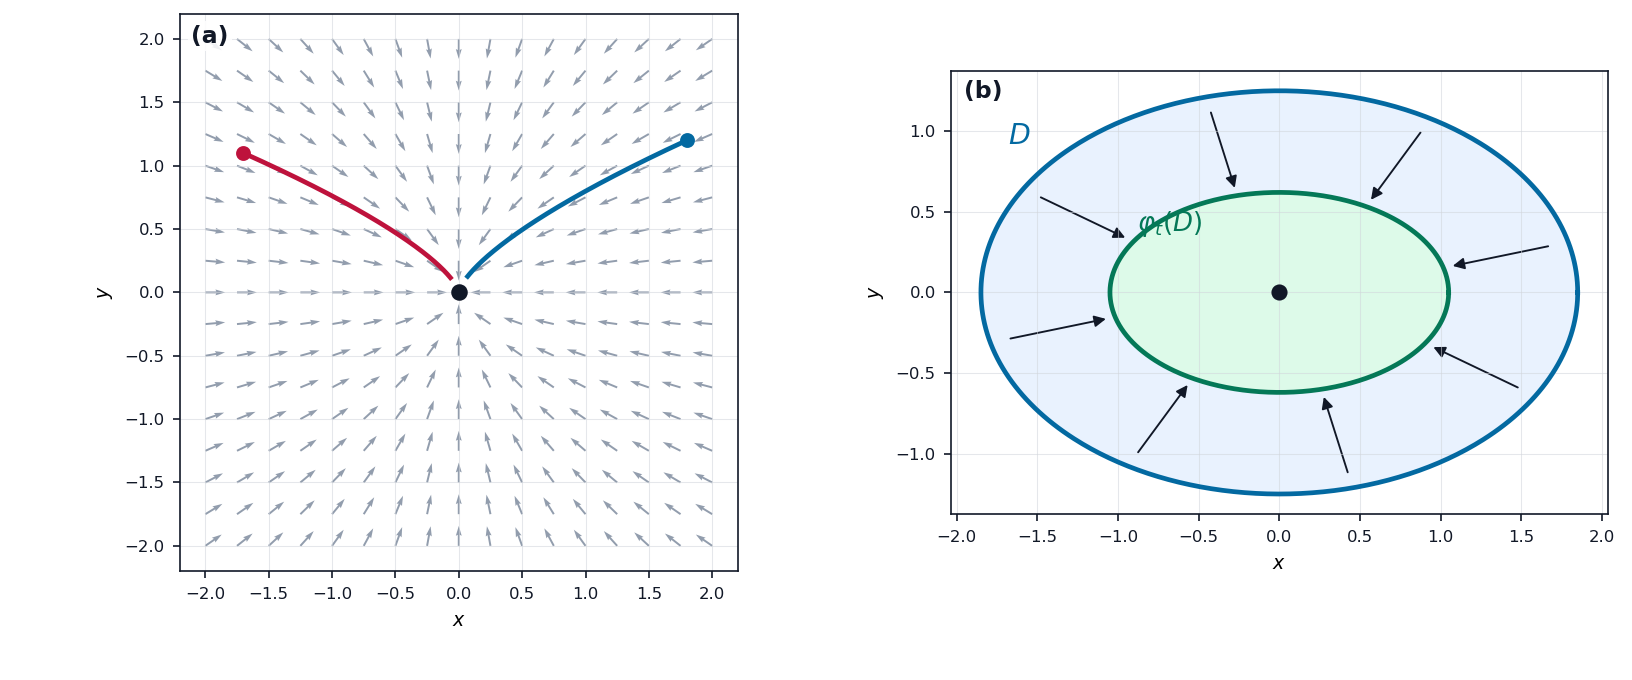
\includegraphics[width=0.90\linewidth]{flow_invariance_trapping.png}
\caption{Dos lecturas complementarias del flujo contractivo: (a) órbitas orientadas
por el campo y (b) transporte de una región $D$ hacia $\varphi_t(D)$. Que la imagen
quede contenida en $D$ expresa invariancia positiva de la región, no invariancia de
cada curva dibujada en su interior.}
\label{fig:gt-flujo-invariancia}
\end{figure}

\lecturaseccion{Jessica Angélica Jaurez Rosas, Laura Ortiz Bobadilla, Jesús Alberto
Palma Márquez y Ernesto Rosales González, \emph{Teoría geométrica de ecuaciones
diferenciales I}, capítulos sobre existencia, unicidad y flujo; Steven H. Strogatz,
\emph{Nonlinear Dynamics and Chaos}, capítulos 2 y 5.}

\subsection{Conjuntos límite, atracción y regiones atrapantes}

Una trayectoria larga puede continuar moviéndose aunque deje de visitar regiones
nuevas. El conjunto $\omega$-límite registra lo que permanece accesible a tiempos
arbitrariamente grandes:

\begin{equation}
 \omega(x)=\bigcap_{T\geq0}
 \overline{\{\Phi_t(x):t\geq T\}}.
 \label{eq:gt-omega}
\end{equation}

Si la semiórbita positiva está contenida en un compacto, $\omega(x)$ no es vacío,
es compacto y es positivamente invariante. El descarte de un transitorio en el
software aproxima la operación $t\geq T$, pero una ventana finita no ejecuta la
intersección para todos los $T$.

\paragraph{Atracción y cuenca.}
Sea $A$ un compacto invariante. Se dice que atrae a $x$ si

\begin{equation}
 \dist(\Phi_t(x),A)\longrightarrow0\qquad(t\to\infty).
 \label{eq:gt-atraccion}
\end{equation}

La cuenca correspondiente es

\begin{equation}
 \mathcal B(A)=\{x:\dist(\Phi_t(x),A)\to0\}.
 \label{eq:gt-cuenca}
\end{equation}

Esta definición separa el conjunto asintótico de los estados que llegan a él. Dos
atractores geométricamente parecidos pueden tener cuencas muy distintas; una cuenca
extensa tampoco vuelve más compleja la dinámica que ocurre dentro del atractor.

\paragraph{Región atrapante.}
Un compacto $N$ es atrapante si existe $t_*>0$ tal que
$\Phi_{t_*}(N)\subset\operatorname{int}N$. El conjunto

\begin{equation}
 A_N=\bigcap_{t\geq0}\Phi_t(N)
 \label{eq:gt-maximo-invariante}
\end{equation}

es el máximo conjunto invariante que permanece dentro de $N$, siempre que el flujo y
la compacidad permitan esta construcción. La región atrapante brinda una cota global;
requiere diagnósticos adicionales para clasificar $A_N$ como equilibrio, ciclo o conjunto más
complicado.

\paragraph{Ejemplo resuelto: oscilación radial autosostenida.}
Considérese

\begin{equation}
 \dot x=x-y-x(x^2+y^2),\qquad
 \dot y=x+y-y(x^2+y^2).
 \label{eq:gt-normal-radial}
\end{equation}

Con $r^2=x^2+y^2$ y $\theta=\operatorname{atan2}(y,x)$,

\begin{equation}
 \dot r=r(1-r^2),\qquad \dot\theta=1.
 \label{eq:gt-radial-polar}
\end{equation}

Para $0<a<1<b$, en $r=a$ se tiene $\dot r>0$ y en $r=b$ se tiene
$\dot r<0$. El anillo $a\leq r\leq b$ es atrapante. Toda condición con $r_0>0$
se aproxima a la circunferencia $r=1$, mientras el origen permanece como equilibrio
inestable. El retrato muestra una espiral hacia una curva cerrada; la serie temporal
muestra una oscilación cuya amplitud se estabiliza; la gráfica de $r(t)$ revela de
forma más directa la atracción radial.

\begin{activitybox}{Práctica reproducible: región atrapante y observable adecuada}
Introduzca \eqref{eq:gt-normal-radial} en \gui{Crear sistema} con variables
\code{x,y}, RK4, $h=0.01$ y $T=25$. Simule desde $(0.2,0)$, $(0.8,0)$,
$(1.4,0)$ y $(2,0)$. Use \gui{Retratos 2D} y \gui{Series temporales}; exporte
los datos y añada la columna $r=\sqrt{x^2+y^2}$. Compare $r(t)$ con la predicción
de signos de \eqref{eq:gt-radial-polar}. Repita con $h/2$ y registre el máximo de
$|r(t)-1|$ en la última cuarta parte de la simulación.
\end{activitybox}

\paragraph{Lectura de una cuenca calculada.}
Cada celda representa una condición inicial y una clasificación obtenida con un
horizonte, un paso y tolerancias. Una franja de celdas sin clasificación estable puede
deberse a una frontera fina, a transitorios largos o a un criterio demasiado rígido.
Antes de describir geometría, conviene seleccionar puntos a ambos lados de la franja,
duplicar el horizonte y refinar la malla localmente.

\begin{figure}[H]
\centering
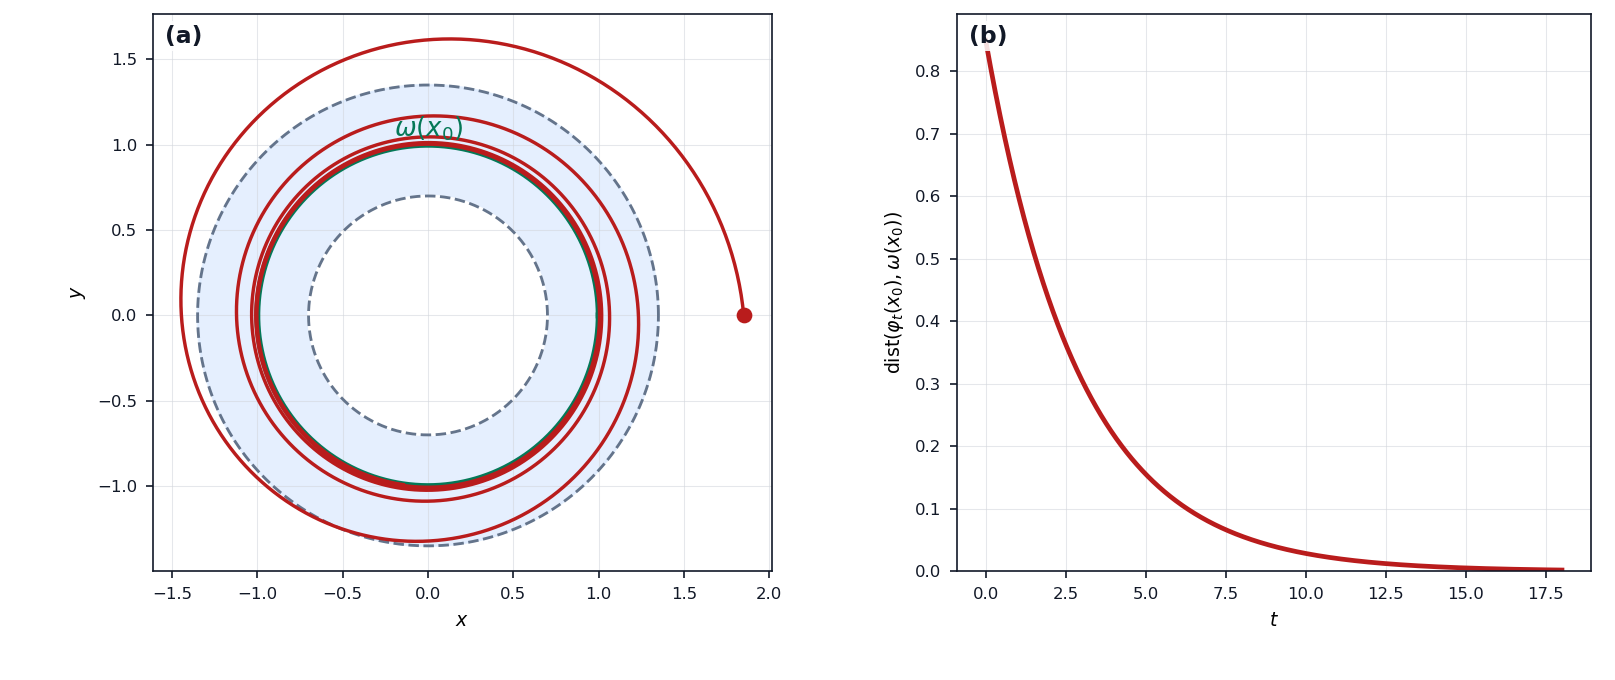
\includegraphics[width=0.90\linewidth]{omega_limit_trapping_region.png}
\caption{Región atrapante y conjunto $\omega$-límite del ejemplo radial: (a) una
órbita entra al anillo y se aproxima al ciclo $r=1$; (b) la distancia al conjunto
límite decrece sin que la trayectoria converja a un punto fijo. La segunda vista
evita confundir atracción hacia un conjunto con convergencia de cada coordenada.}
\label{fig:gt-omega-atrapante}
\end{figure}

\lecturaseccion{Kathleen T. Alligood, Tim D. Sauer y James A. Yorke,
\emph{Chaos: An Introduction to Dynamical Systems}, secciones sobre conjuntos
límite, cuencas y fronteras; Tamás Tél y Márton Gruiz, \emph{Chaotic Dynamics: An
Introduction Based on Classical Mechanics}, capítulos sobre dinámica transitoria y
cuencas.}

\subsection{Conjugación topológica y equivalencia orbital}

Dos ecuaciones escritas de forma distinta pueden representar la misma organización de
órbitas. La noción precisa depende de cuánto se desea conservar.

\paragraph{Conjugación.}
Los flujos $\Phi_t$ sobre $X$ y $\Psi_t$ sobre $Y$ son topológicamente conjugados si
existe un homeomorfismo $h:X\to Y$ tal que

\begin{equation}
 h\circ\Phi_t=\Psi_t\circ h
 \qquad\text{para todo }t.
 \label{eq:gt-conjugacion}
\end{equation}

La conjugación conserva el reloj: estados correspondientes se observan en el mismo
tiempo. Transporta equilibrios, periodicidad, invariancia y estructura de conjuntos
límite. No conserva longitudes, ángulos ni tasas expresadas en una métrica arbitraria.

Si $h$ es un difeomorfismo y $y=h(x)$, la regla de la cadena da el campo transformado

\begin{equation}
 g(y)=Dh(h^{-1}(y))f(h^{-1}(y)).
 \label{eq:gt-empuje-campo}
\end{equation}

El factor $Dh$ es esencial. Cambiar sólo el nombre de las variables no transporta el
campo.

\paragraph{Equivalencia orbital.}
Si se permite una reparametrización creciente del tiempo, basta que $h$ lleve órbitas
orientadas en órbitas orientadas. Multiplicar el campo por una función positiva
$\alpha(x)$,

\begin{equation}
 \dot x=\alpha(x)f(x),\qquad \alpha(x)>0,
 \label{eq:gt-reparametrizacion}
\end{equation}

conserva las curvas integrales orientadas, pero cambia la rapidez con que se recorren.
Por eso la equivalencia orbital no conserva periodos ni exponentes por unidad de
tiempo.

\paragraph{Ejemplo de conjugación lineal.}
Para $\dot x=-x$, la solución es $x(t)=e^{-t}x_0$. Tome
$h(x)=x^3$, homeomorfismo de $\R$. Entonces

\begin{equation}
 y(t)=h(x(t))=e^{-3t}y_0,\qquad \dot y=-3y.
 \label{eq:gt-conjugacion-cubica}
\end{equation}

Los dos flujos son conjugados por $h$: tienen un equilibrio globalmente atractivo y la
misma organización de semiórbitas. Sus tasas lineales son diferentes. El ejemplo
advierte que una tasa numérica se presenta con su métrica y sus unidades, en vez de como invariante topológico.

\begin{activitybox}{Ejercicio con pista: transporte de una región}
Sea $x=Tz+c$, con $T$ invertible. Demuestre que la bola
$\|x-x_e\|_2\leq r$ se transforma en
$(z-z_e)^{\mathsf T}T^{\mathsf T}T(z-z_e)\leq r^2$.
Explique por qué una malla cuadrada en las coordenadas $z$ no representa en general
una malla cuadrada en $x$. \textbf{Pista:} sustituya
$x-x_e=T(z-z_e)$ antes de elevar la norma al cuadrado.
\end{activitybox}

\paragraph{Interpretación de gráficas comparadas.}
Dos retratos conjugados pueden verse estirados, inclinados o curvados. Lo importante
es si conservan la correspondencia entre órbitas, equilibrios y conexiones. Si además
se comparan series temporales, hay que aclarar si el reloj se conservó. Superponer
curvas sin transportar coordenadas y tiempo mezcla dos preguntas distintas.

\begin{figure}[H]
\centering
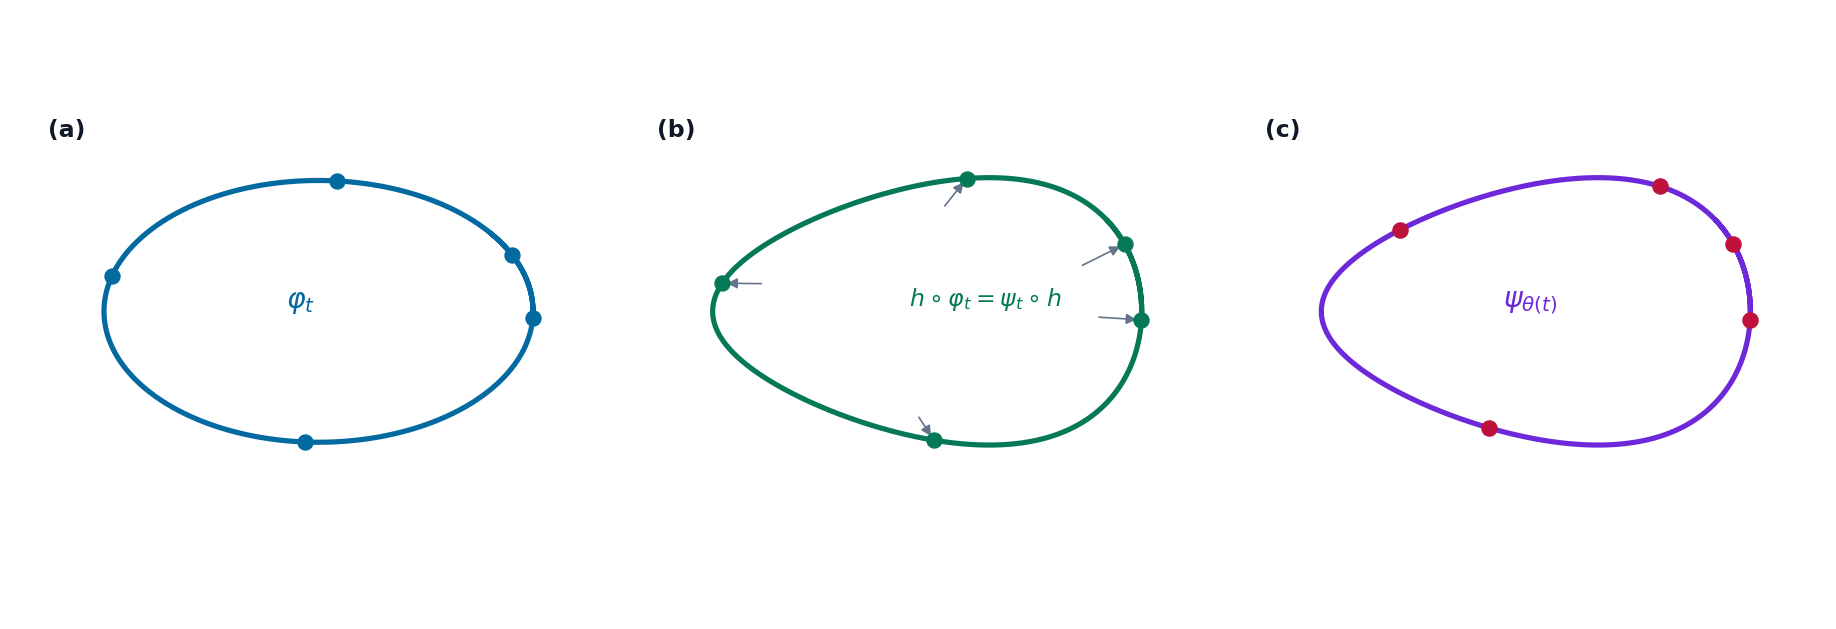
\includegraphics[width=0.92\linewidth]{conjugacy_orbital_equivalence.png}
\caption{Correspondencias de órbitas: (a) una órbita de $\varphi_t$, (b) su
deformación por un homeomorfismo $h$ con las mismas marcas temporales y (c) la misma
órbita geométrica con marcas redistribuidas por $\theta(t)$. El último panel ilustra
por qué equivalencia orbital conserva el recorrido, pero no necesariamente el reloj.}
\label{fig:gt-conjugacion-orbital}
\end{figure}

\lecturaseccion{Morris W. Hirsch, Stephen Smale y Robert L. Devaney,
\emph{Differential Equations, Dynamical Systems, and an Introduction to Chaos},
capítulos sobre equivalencia y linealización; John Guckenheimer y Philip Holmes,
\emph{Nonlinear Oscillations, Dynamical Systems, and Bifurcations of Vector Fields},
capítulo 1.}

\subsection{Variación, cambio de volumen y variedades invariantes}

Una trayectoria describe la evolución de un estado. Para estudiar la evolución de
una perturbación se deriva el flujo respecto de la condición inicial. Si
$x(t)=\Phi_t(x_0)$ y $f$ es diferenciable, la matriz fundamental

\begin{equation}
 M(t)=D_{x_0}\Phi_t(x_0)
 \label{eq:gt-matriz-fundamental}
\end{equation}

satisface la ecuación variacional

\begin{equation}
 \dot M(t)=Df(x(t))M(t),\qquad M(0)=I.
 \label{eq:gt-variacional}
\end{equation}

Una perturbación pequeña se aproxima por $\delta x(t)=M(t)\delta x_0$. Los valores
singulares de $M(t)$ describen los ejes principales del elipsoide obtenido al deformar
una esfera infinitesimal. Los exponentes finitos se calculan a partir de sus tasas
logarítmicas, pero dependen del horizonte y del tratamiento numérico.

\paragraph{Fórmula de Liouville.}
La identidad de Jacobi para el determinante da

\begin{equation}
 \frac{\dd}{\dd t}\det M
 =\det M\,\operatorname{tr}(M^{-1}\dot M).
 \label{eq:gt-jacobi-det}
\end{equation}

Al sustituir \eqref{eq:gt-variacional},
$M^{-1}\dot M=M^{-1}Df(x(t))M$, cuya traza es
$\operatorname{tr}Df(x(t))=\nabla\cdot f(x(t))$. Por integración,

\begin{equation}
 \det M(t)=
 \exp\left(\int_0^t\nabla\cdot f(x(s))\dd s\right).
 \label{eq:gt-liouville}
\end{equation}

La divergencia mide expansión instantánea de volumen. Divergencia negativa implica
contracción de elementos de volumen a lo largo del flujo, pero no identifica por sí
sola el conjunto al que llegan las trayectorias ni prueba que una región particular
sea atrapante.

\paragraph{Equilibrio hiperbólico y variedades.}
Un equilibrio $e$ es hiperbólico si $Df(e)$ no tiene valores propios con parte real
cero. El espacio tangente se separa como

\begin{equation}
 \R^n=E^s\oplus E^u,
 \label{eq:gt-descomposicion-hiperbolica}
\end{equation}

donde $E^s$ corresponde a valores propios con parte real negativa y $E^u$ a parte
real positiva. El teorema de la variedad estable proporciona objetos no lineales
$W^s_{\mathrm{loc}}(e)$ y $W^u_{\mathrm{loc}}(e)$ tangentes a esos subespacios en
$e$. La linealización determina la tangencia local, no la forma global completa.

\paragraph{Ejemplo de variedad invariante curvada.}
Considérese

\begin{equation}
 \dot x=x,\qquad \dot y=-y+x^2.
 \label{eq:gt-silla-no-lineal}
\end{equation}

El origen tiene valores propios $1$ y $-1$. La recta $x=0$ es la variedad estable.
Para buscar la variedad inestable como $y=h(x)=ax^2$, se impone invariancia:

\begin{equation}
 h'(x)\dot x=-h(x)+x^2.
 \label{eq:gt-invariancia-grafica}
\end{equation}

Como $h'(x)\dot x=2ax^2$ y $-h(x)+x^2=(1-a)x^2$, se obtiene
$2a=1-a$ y, por tanto,

\begin{equation}
 W^u_{\mathrm{loc}}(0):\quad y=\frac{x^2}{3}.
 \label{eq:gt-variedad-inestable}
\end{equation}

El subespacio lineal $E^u$ es el eje $x$; la variedad verdadera se separa de él en
orden cuadrático. Un retrato con escala amplia puede hacerlas parecer iguales.

\begin{activitybox}{Práctica reproducible: tangencia local y curvatura}
Defina \eqref{eq:gt-silla-no-lineal} en \gui{Crear sistema}. Use RK4,
$h=0.002$, $T=6$ y condiciones $(0.02,0.02^2/3)$,
$(-0.02,0.02^2/3)$, $(0.02,0)$ y $(0,0.2)$. En \gui{Retratos 2D}, superponga
la parábola $y=x^2/3$ mediante datos exportados o puntos de referencia. Repita con
$h/2$. Describa qué trayectorias permanecen cerca de la parábola y por qué la
proximidad visual se complementa con la ecuación de invariancia.
\end{activitybox}

\begin{figure}[H]
\centering
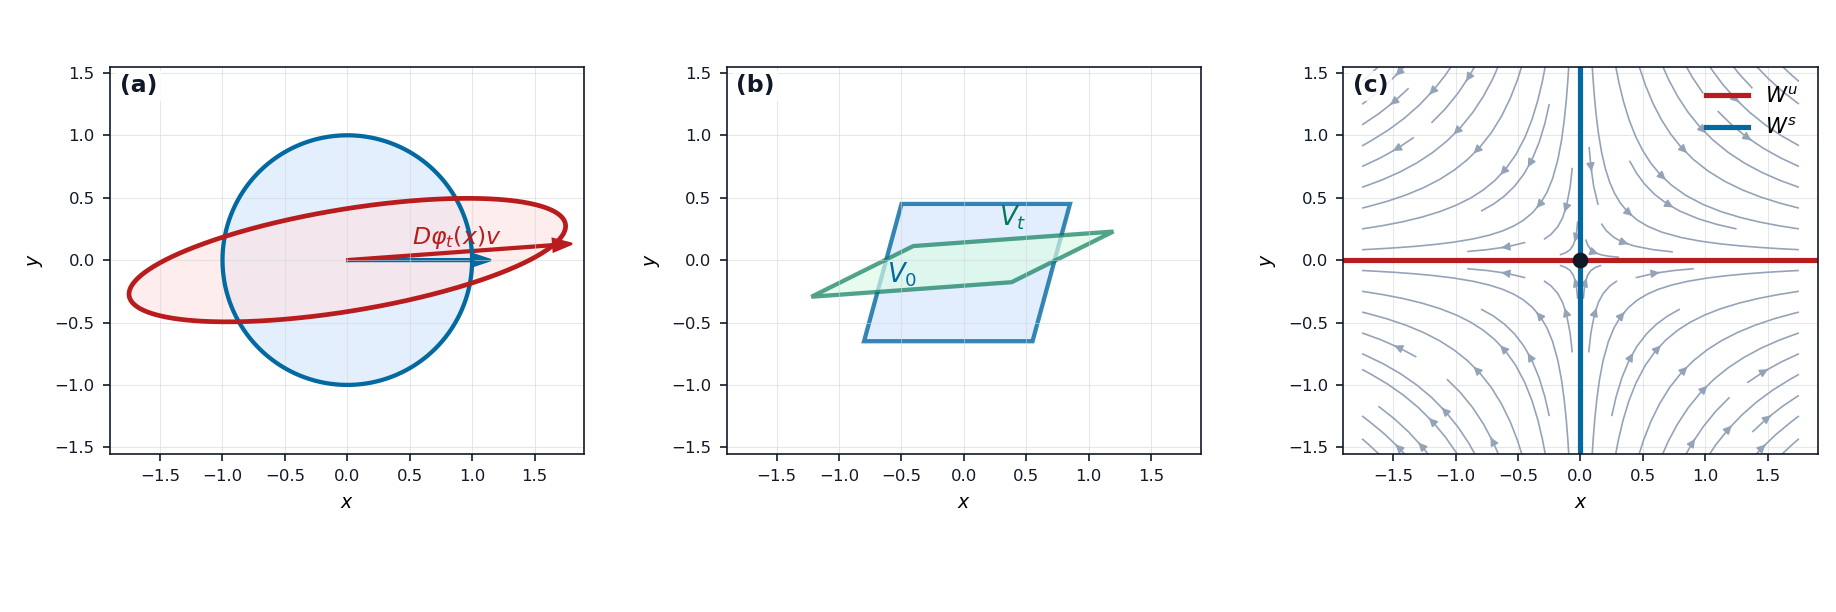
\includegraphics[width=0.94\linewidth]{variational_volume_manifolds.png}
\caption{Tres objetos del sistema variacional: (a) transporte de una perturbación por
$D\varphi_t$, (b) cambio de un elemento de área gobernado por el determinante y
(c) direcciones estable e inestable de una silla. Una elipse o un paralelogramo son
aproximaciones lineales locales; las variedades globales pueden curvarse.}
\label{fig:gt-variacion-volumen-variedades}
\end{figure}

\lecturaseccion{Jessica Angélica Jaurez Rosas, Laura Ortiz Bobadilla, Jesús Alberto
Palma Márquez y Ernesto Rosales González, \emph{Teoría geométrica de ecuaciones
diferenciales II}, secciones sobre primera variación y variedades invariantes; Steven
H. Strogatz, \emph{Nonlinear Dynamics and Chaos}, capítulo 6.}

\subsection{Sección de Poincaré, monodromía y teoría de Floquet}

Una órbita periódica de periodo $T$ es una curva cerrada en el espacio de fases. Para
estudiar su estabilidad se elige una hipersuperficie transversal

\begin{equation}
 \Sigma=\{x:h(x)=0\},\qquad
 \nabla h(x)^{\mathsf T}f(x)\neq0
 \label{eq:gt-seccion}
\end{equation}

en los cruces considerados. El primer retorno lleva $z\in\Sigma$ al siguiente cruce:

\begin{equation}
 P(z)=\Phi_{\tau(z)}(z).
 \label{eq:gt-retorno}
\end{equation}

La órbita periódica se convierte en un punto fijo $P(p)=p$. Si los autovalores de
$DP(p)$ tienen módulo menor que uno, el ciclo es localmente atractivo en direcciones
transversales. Un conjunto de cruces apiñados sugiere un punto fijo; demostrarlo exige
controlar el evento, el tiempo de retorno y el error.

\paragraph{Monodromía y multiplicadores.}
Sobre una solución periódica $\gamma(t)$, la ecuación variacional tiene coeficientes
periódicos:

\begin{equation}
 \dot M(t)=Df(\gamma(t))M(t),\qquad M(0)=I.
 \label{eq:gt-variacional-periodica}
\end{equation}

La matriz $M(T)$ es la matriz de monodromía y sus autovalores son los multiplicadores
de Floquet. En un flujo autónomo aparece un multiplicador $1$ asociado al
desplazamiento a lo largo de la órbita. Los multiplicadores restantes miden el
comportamiento transversal y coinciden, bajo las identificaciones apropiadas, con los
autovalores de $DP(p)$.

En un sistema plano, Liouville permite obtener el multiplicador transversal sin
integrar toda la matriz:

\begin{equation}
 \mu_\perp=
 \exp\left(\int_0^T\nabla\cdot f(\gamma(t))\dd t\right).
 \label{eq:gt-multiplicador-planar}
\end{equation}

\paragraph{Ejemplo de multiplicadores de Floquet.}
En \eqref{eq:gt-normal-radial}, el ciclo $r=1$ tiene periodo $T=2\pi$. Si
$r=1+\eta$, entonces

\begin{equation}
 \dot\eta=\left.\frac{\dd}{\dd r}[r(1-r^2)]\right|_{r=1}\eta
 +O(\eta^2)=-2\eta+O(\eta^2).
 \label{eq:gt-variacion-radial}
\end{equation}

Después de una vuelta, $\eta(T)\simeq e^{-4\pi}\eta(0)$; por tanto,
$\mu_\perp=e^{-4\pi}$ y el ciclo es fuertemente atractivo en dirección radial.
La curva cerrada del retrato no muestra por sí sola ese número: hace falta comparar
retornos o resolver la variación.

\begin{activitybox}{Práctica reproducible: construir un retorno desde datos}
Use la trayectoria de \eqref{eq:gt-normal-radial} con $(x_0,y_0)=(1.4,0.1)$,
RK4, $h=0.005$ y $T=30$. Exporte el CSV. Detecte cruces de $y<0$ a $y\geq0$
con $x>0$ e interpole linealmente el valor de $x$ en cada cruce. Construya
$x_{k+1}$ contra $x_k$ y compare $|x_k-1|$ entre vueltas consecutivas. Repita con
$h/2$. Informe el cociente tardío y compárelo con $e^{-4\pi}$, señalando la
limitación de la interpolación de eventos.
\end{activitybox}

\paragraph{Lectura de la gráfica de retorno.}
La diagonal $P(z)=z$ permite localizar puntos fijos. La pendiente indica estabilidad
en un mapa escalar: $|P'(z^*)|<1$ atrae y $|P'(z^*)|>1$ repele. Una nube gruesa puede
proceder de dinámica compleja, de una sección mal definida, de cruces tangenciales o
de muestreo insuficiente. Antes de interpretarla, deben revisarse orientación,
transitorio y refinamiento del instante de cruce.

\begin{figure}[H]
\centering
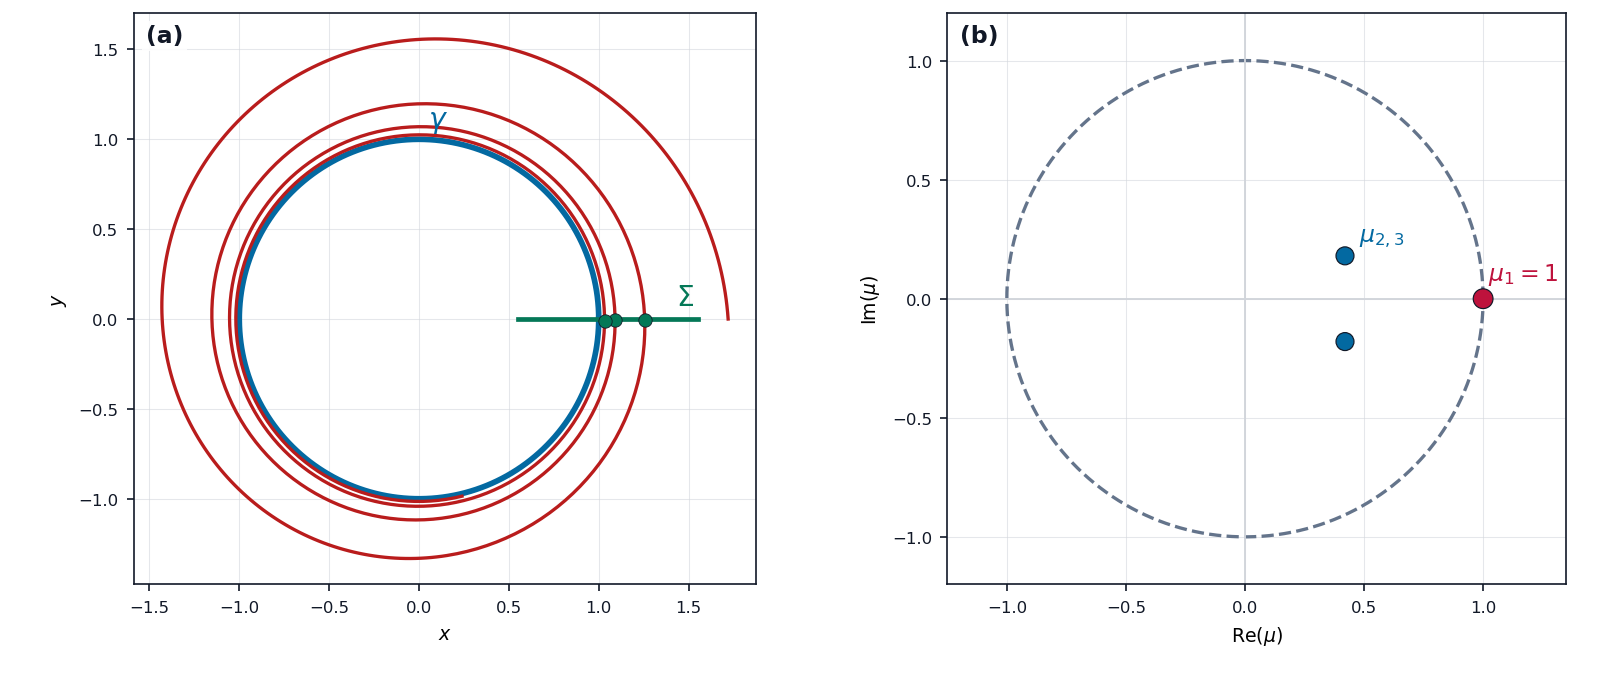
\includegraphics[width=0.90\linewidth]{poincare_floquet_geometry.png}
\caption{Geometría de retorno y estabilidad orbital: (a) una sección transversal
$\Sigma$ reduce el ciclo $\gamma$ a iteraciones discretas; (b) los multiplicadores de
Floquet se leen respecto del círculo unidad. El multiplicador trivial $\mu_1=1$
corresponde al desplazamiento de fase y no decide la estabilidad transversal.}
\label{fig:gt-poincare-floquet}
\end{figure}

\lecturaseccion{Frank C. Hoppensteadt, \emph{Analysis and Simulation of Chaotic
Systems}, secciones sobre estabilidad orbital y mapas de retorno; John Guckenheimer y
Philip Holmes, \emph{Nonlinear Oscillations, Dynamical Systems, and Bifurcations of
Vector Fields}, capítulos 1--3.}

\subsection{Grado, puntos fijos y existencia}

Los métodos topológicos de existencia no buscan necesariamente una fórmula cerrada.
Transforman el problema en un cero o un punto fijo y usan continuidad, compacidad y
comportamiento en la frontera para demostrar que el objeto debe existir.

\paragraph{Contracción.}
En un espacio métrico completo, una aplicación $T$ es contractiva si existe
$0<L<1$ tal que

\begin{equation}
 d(Tx,Ty)\leq Ld(x,y).
 \label{eq:gt-contraccion}
\end{equation}

El teorema de Banach garantiza un único punto fijo y la convergencia de
$x_{n+1}=T(x_n)$. La conclusión combina existencia, unicidad y un algoritmo; si sólo
se sabe que $T$ es continua sobre una región compacta, esas tres propiedades no se
obtienen juntas.

\paragraph{Brouwer y grado.}
Toda aplicación continua de una bola cerrada de $\R^n$ en sí misma posee un punto
fijo. El grado de Brouwer refina esta idea. Para
$F:\overline\Omega\to\R^n$ y $0\notin F(\partial\Omega)$ se define un entero
$\deg(F,\Omega,0)$. Si es distinto de cero, $F$ tiene al menos un cero en
$\Omega$. Cuando los ceros son regulares y finitos,

\begin{equation}
 \deg(F,\Omega,0)=
 \sum_{x\in F^{-1}(0)\cap\Omega}
 \operatorname{sgn}\det DF(x).
 \label{eq:gt-grado-regular}
\end{equation}

El grado se conserva durante una homotopía $F_\lambda$ mientras ningún cero cruce la
frontera. Garantiza existencia, pero no decide estabilidad ni describe la cuenca.

\paragraph{Ejemplo de punto fijo por contracción.}
Para $F(x)=x-x^3$ en $\Omega=(-2,2)$, los ceros son $-1,0,1$ y
$F'(x)=1-3x^2$. La suma de signos es

\begin{equation}
 \deg(F,(-2,2),0)=(-1)+(+1)+(-1)=-1.
 \label{eq:gt-grado-cubico}
\end{equation}

El grado no nulo obliga a conservar al menos un cero bajo toda deformación admisible.
Para saber cuáles de esos equilibrios atraen se necesita el signo de la linealización
o un argumento no lineal adicional.

\paragraph{Disparo y residual de retorno.}
En el problema de frontera

\begin{equation}
 u''=G(t,u,u'),\qquad u(0)=a,\qquad u(T)=b,
 \label{eq:gt-problema-frontera}
\end{equation}

se elige la pendiente inicial $s=u'(0)$ y se define

\begin{equation}
 S(s)=u(T;s)-b.
 \label{eq:gt-residual-disparo}
\end{equation}

Un cero de $S$ resuelve el problema. Para una órbita periódica se usa de manera
análoga el residual $R(z)=P(z)-z$. Aplicar grado a $R$ requiere que el retorno exista
y sea continuo en la región; el cálculo de retornos debe acompañarse de la verificación explícita de esas hipótesis.

\begin{activitybox}{Ejercicios con pistas: tres formas de existencia}
\textbf{1.} Resuelva por disparo $u''+u=0$, $u(0)=0$,
$u(\pi/2)=1$. \textbf{Pista:} con pendiente $s$, $u(t;s)=s\sin t$.

\textbf{2.} Si $P:[a,b]\to[a,b]$ es continuo, pruebe que tiene un punto fijo.
\textbf{Pista:} estudie los signos de $P(x)-x$ en los extremos.

\textbf{3.} Calcule el grado de $x^3-x$ en intervalos pequeños alrededor de cada
raíz y verifique aditividad al reunirlos.
\end{activitybox}

\begin{figure}[H]
\centering
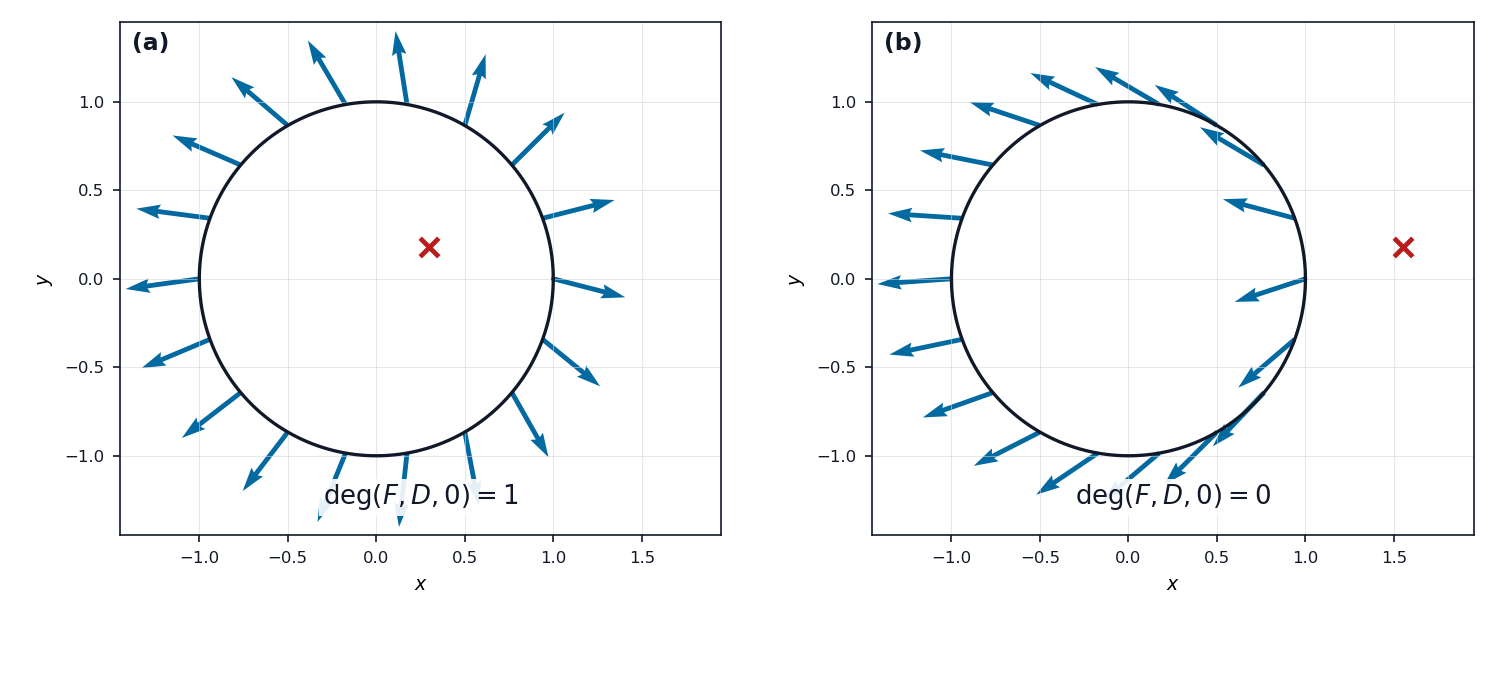
\includegraphics[width=0.82\linewidth]{degree_fixed_point.png}
\caption{Lectura geométrica del grado en el plano: el campo sobre la frontera rodea
una vez al origen cuando el cero está dentro de $D$ y no lo rodea cuando está fuera.
El dibujo orienta el cálculo; la conclusión de existencia requiere continuidad y
ausencia de ceros sobre la frontera.}
\label{fig:gt-grado-existencia}
\end{figure}

\lecturaseccion{Pablo Gustavo Amster, \emph{Métodos topológicos en el estudio de las
ecuaciones diferenciales no lineales}, capítulos sobre disparo, punto fijo y grado;
Jessica Angélica Jaurez Rosas et al., \emph{Teoría geométrica de ecuaciones
diferenciales II}, secciones sobre existencia y continuación.}

\subsection{Homoclinicidad, herradura y dinámica simbólica}

Una conexión homoclínica aparece cuando una órbita sale de un objeto hiperbólico por
su variedad inestable y regresa por su variedad estable. En un mapa, si $p$ es un
punto fijo hiperbólico, una intersección

\begin{equation}
 q\in W^s(p)\cap W^u(p),\qquad
 T_qW^s+T_qW^u=T_qX,
 \label{eq:gt-homoclinica-transversal}
\end{equation}

es transversal. La transversalidad impide que la intersección desaparezca ante una
perturbación pequeña. El teorema de Smale--Birkhoff establece que una intersección
homoclínica transversal de un punto periódico hiperbólico genera, para alguna
iteración, una dinámica tipo herradura sobre un conjunto invariante.

\paragraph{Estirar, contraer y plegar.}
La herradura toma una región, la estira en una dirección, la contrae en otra y la
pliega de modo que dos tiras regresan a la región inicial. Cada órbita que permanece
en el conjunto puede codificarse según la tira visitada:

\begin{equation}
 \ldots s_{-1}.s_0s_1s_2\ldots,\qquad s_k\in\{0,1\}.
 \label{eq:gt-codigo-simbolico}
\end{equation}

El corrimiento $\sigma$ elimina el símbolo presente y desplaza la secuencia. En una
métrica como

\begin{equation}
 d(s,r)=\sum_{k\in\mathbb Z}\frac{|s_k-r_k|}{2^{|k|+1}},
 \label{eq:gt-metrica-secuencias}
\end{equation}

dos secuencias son próximas si coinciden alrededor del presente. El corrimiento posee
órbitas periódicas densas, transitividad y sensibilidad. Esta construcción transforma
geometría de intersecciones en una descripción combinatoria.

\paragraph{Definiciones de caos.}
Para un mapa continuo sobre un conjunto invariante, la definición de Devaney combina
transitividad, densidad de puntos periódicos y sensibilidad. La entropía topológica
mide crecimiento de órbitas distinguibles. Un exponente de Lyapunov positivo mide
expansión promedio a lo largo de una trayectoria. Estas nociones se relacionan en
contextos precisos, y cada una conserva su ámbito de aplicación.

\paragraph{Evidencia requerida para interpretar una figura.}
Un pliegue visible sugiere buscar variedades e intersecciones. Una nube de retornos
sugiere estudiar un mapa iterado. Una banda ancha sugiere ausencia de una frecuencia
dominante simple. Ninguna de esas señales encierra por sí misma una intersección
transversal, una conjugación con el corrimiento o un valor exacto de entropía.

\begin{activitybox}{Práctica reproducible: itinerarios del mapa logístico}
En \gui{Bifurcación} seleccione \gui{Logistico [listo]}, use $x_0=0.2$ y estudie
primero $r=3.2$ y después $r=4$. Para cada valor conserve 200 iteraciones después de
descartar 1000. Exporte la sucesión y codifique $s_n=0$ si $x_n<1/2$ y $s_n=1$ si
$x_n\geq1/2$. Repita desde $x_0+10^{-8}$. Compare la longitud del prefijo común,
los bloques de símbolos y los puntos del retrato $x_{n+1}$ contra $x_n$. Esta
práctica estudia itinerarios finitos; no presenta la muestra como demostración de una
conjugación global.
\end{activitybox}

\begin{activitybox}{Ejercicio con pista: periodicidad simbólica}
Construya las secuencias binarias de periodo primo $1$, $2$ y $3$ bajo el corrimiento.
¿Cuántas palabras de longitud $n$ existen antes de identificar rotaciones?
\textbf{Pista:} hay $2^n$ palabras; para contar órbitas de periodo primo hay que
eliminar palabras de periodo divisor y después identificar desplazamientos cíclicos.
\end{activitybox}

\begin{figure}[H]
\centering
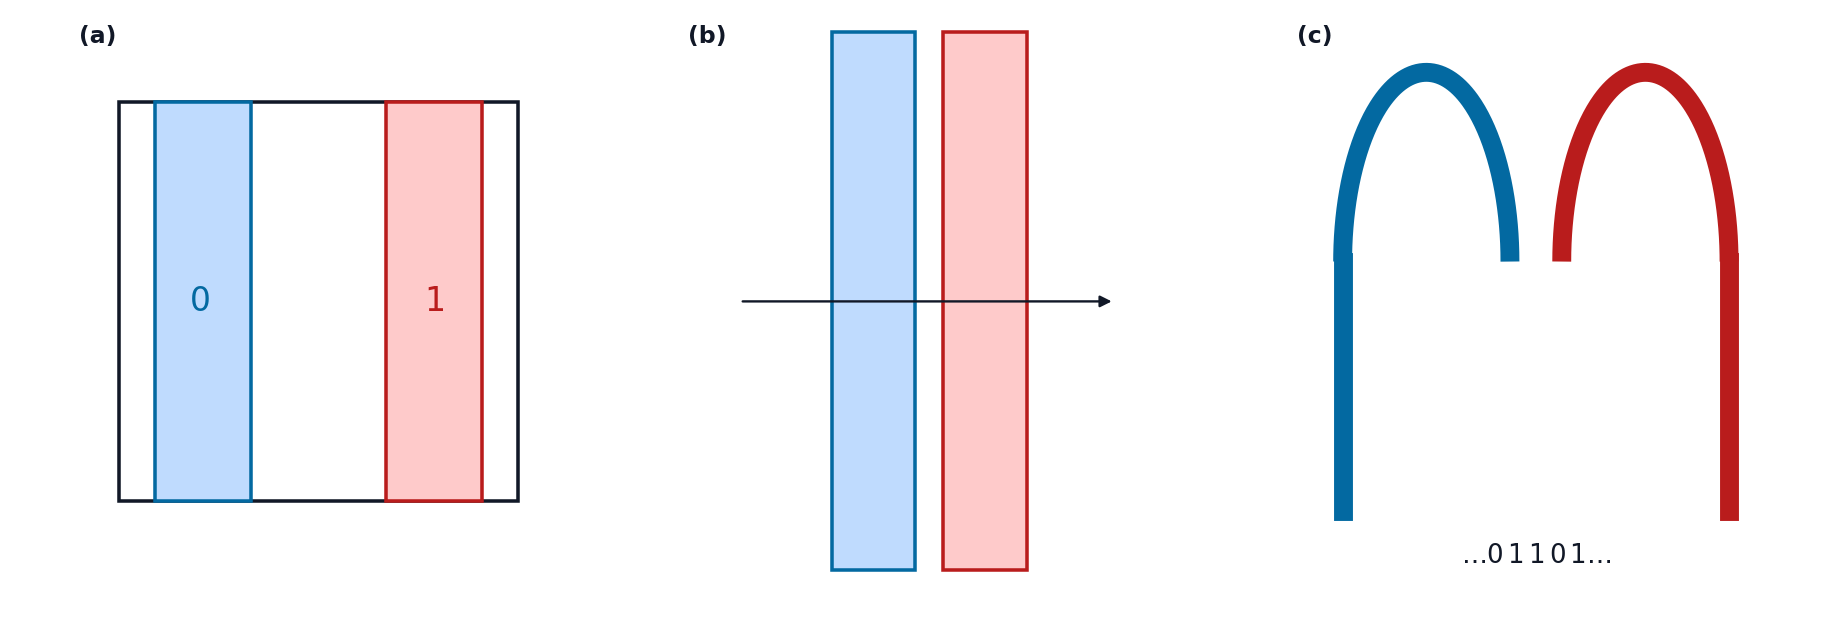
\includegraphics[width=0.92\linewidth]{horseshoe_symbolic_dynamics.png}
\caption{Esquema docente de la herradura: (a) dos franjas codificadas, (b)
estiramiento y contracción, y (c) plegamiento con un itinerario binario asociado.
La figura explica el mecanismo y la codificación; verificar una herradura en un
sistema concreto exige construir el mapa y demostrar las intersecciones necesarias.}
\label{fig:gt-herradura-simbolica}
\end{figure}

\lecturaseccion{Robert L. Devaney, \emph{An Introduction to Chaotic Dynamical
Systems}, capítulos sobre dinámica simbólica; Morris W. Hirsch, Stephen Smale y
Robert L. Devaney, \emph{Differential Equations, Dynamical Systems, and an
Introduction to Chaos}, capítulos 15--16; Kathleen T. Alligood, Tim D. Sauer y James
A. Yorke, \emph{Chaos: An Introduction to Dynamical Systems}, capítulos sobre
herraduras y órbitas homoclínicas.}

\subsection{Estados con memoria y derivadas fraccionarias}

En una ODE autónoma, conocer $x(t)$ basta para continuar la solución porque la ley de
flujo permite reiniciar desde ese estado. Una ecuación de Caputo conserva información
del intervalo recorrido desde el terminal inferior. Para $0<q<1$,

\paragraph{Función Gamma e integración fraccionaria.}
La función Gamma prolonga el factorial y fija la normalización de los operadores:

\begin{equation}
 \Gamma(z)=\int_0^\infty s^{z-1}e^{-s}\dd s,
 \qquad \Gamma(z+1)=z\Gamma(z).
 \label{eq:gt-gamma}
\end{equation}

Para $\alpha>0$, la integral izquierda de Riemann--Liouville con terminal inferior
$t_0$ es

\begin{equation}
 (I_{t_0}^{\alpha}g)(t)=\frac{1}{\Gamma(\alpha)}
 \int_{t_0}^{t}(t-s)^{\alpha-1}g(s)\dd s.
 \label{eq:gt-integral-rl}
\end{equation}

La identidad beta--Gamma permite probar, bajo condiciones de integrabilidad que
justifican intercambiar el orden de integración,

\begin{equation}
 I_{t_0}^{\alpha}I_{t_0}^{\beta}=I_{t_0}^{\alpha+\beta}.
 \label{eq:gt-semigrupo-orden}
\end{equation}

La composición ocurre respecto del orden del operador. Su interpretación difiere de la composición
temporal para el estado de un problema con memoria. Distinguir ambas afirmaciones
evita atribuir a la solución una propiedad que sólo pertenece a las integrales.

\paragraph{Definiciones de derivada fraccionaria.}
Si $m-1<q<m$, las derivadas de Riemann--Liouville y de Caputo ordenan de modo
distinto la derivación entera y la integración fraccionaria:

\begin{equation}
 {}^{\mathrm{RL}}D_{t_0}^{q}x
 =\frac{\dd^m}{\dd t^m}I_{t_0}^{m-q}x,
 \qquad
 {}^{\mathrm C}D_{t_0}^{q}x
 =I_{t_0}^{m-q}x^{(m)}.
 \label{eq:gt-rl-caputo}
\end{equation}

Para $0<q<1$, Caputo anula una constante, mientras

\begin{equation}
 {}^{\mathrm{RL}}D_{t_0}^{q}c
 =\frac{c(t-t_0)^{-q}}{\Gamma(1-q)}.
 \label{eq:gt-rl-constante}
\end{equation}

La forma de Grünwald--Letnikov aproxima el operador mediante diferencias de todos los
pasos anteriores:

\begin{equation}
 {}^{\mathrm{GL}}D_{t_0}^{q}x(t_n)
 \approx h^{-q}\sum_{j=0}^{n}(-1)^j
 \binom{q}{j}x(t_{n-j}),
 \qquad
 \binom{q}{j}=\frac{\Gamma(q+1)}{\Gamma(j+1)\Gamma(q-j+1)}.
 \label{eq:gt-gl-discreta}
\end{equation}

Estas expresiones describen operadores distintos. Deben declararse el
operador, el terminal inferior, la regularidad y la información inicial. Caputo es
conveniente cuando se formulan datos ordinarios $x(t_0)$; Riemann--Liouville puede
requerir datos expresados mediante integrales fraccionarias; Grünwald--Letnikov ofrece
una ruta discreta que vuelve explícito el costo de conservar la historia.

\begin{activitybox}{Ejercicio de lectura activa: una potencia como banco de prueba}
Para $x(t)=(t-t_0)^\nu$, con $\nu>0$, use la identidad beta--Gamma para obtener
la integral \eqref{eq:gt-integral-rl} y después las derivadas de
Riemann--Liouville y Caputo cuando existan. Verifique por separado el caso constante.
Compare la fórmula con \eqref{eq:gt-gl-discreta} para $q=0.6$, $h=0.1,0.05$ y
$t-t_0=1$. La entrega debe indicar dominio de los parámetros y error relativo, no
sólo valores decimales.
\end{activitybox}

\lecturaseccion{Shantanu Das, \emph{Kindergarten of Fractional Calculus}, capítulos
1--3, para Gamma, generalización, integración y las formas de Grünwald--Letnikov,
Riemann--Liouville y Caputo; Edmundo Capelas de Oliveira, \emph{Solved Exercises in
Fractional Calculus}, capítulos 2--5, para funciones especiales, Mittag--Leffler,
transformadas y comparación de operadores.}

\paragraph{Terminal inferior e inicialización.}
El valor $t_0$ marca el comienzo de la memoria
incluida en el modelo. Cambiarlo modifica el operador. Si el proceso ya tenía historia
antes de $t_0$, esa preparación debe incorporarse mediante un término de
inicialización o una historia declarada. Reiniciar el cálculo en un tiempo intermedio
con el transporte de esa información se define un problema equivalente. La pregunta correcta se formula como
únicamente cuál es $x(t_0)$, sino qué preparación representa el dato inicial y desde
qué instante se acumula la memoria.

\lecturaseccion{Shantanu Das, \emph{Kindergarten of Fractional Calculus}, capítulo 5,
sobre inicialización; Richard Herrmann, \emph{Fractional Calculus: An Introduction
for Physicists}, capítulo 8, sobre no localidad y memoria.}

Con este marco, la derivada de Caputo de orden $0<q<1$ se escribe

\begin{equation}
 {}^{\mathrm C}D_{0+}^{q}x(t)
 =\frac{1}{\Gamma(1-q)}
 \int_0^t(t-s)^{-q}\dot x(s)\dd s.
 \label{eq:gt-caputo}
\end{equation}

El problema

\begin{equation}
 {}^{\mathrm C}D_{0+}^{q}x(t)=f(x(t)),\qquad x(0)=x_0
 \label{eq:gt-pvi-caputo}
\end{equation}

es equivalente, bajo las hipótesis habituales, a la ecuación de Volterra

\begin{equation}
 x(t)=x_0+\frac{1}{\Gamma(q)}
 \int_0^t(t-s)^{q-1}f(x(s))\dd s.
 \label{eq:gt-volterra}
\end{equation}

La equivalencia se obtiene aplicando la integral fraccionaria de orden $q$ y usando
$I^q\,{}^{\mathrm C}D^qx=x-x_0$. La integral de Volterra muestra la memoria de forma
directa: cada valor pasado del campo participa en la continuación con un peso que
depende de la distancia temporal.

\paragraph{Perfil de memoria.}
Fije un tiempo $t$ y escriba el futuro como $t+\theta$. Al separar
\eqref{eq:gt-volterra} en $[0,t]$ y $[t,t+\theta]$, se obtiene

\begin{align}
 x(t+\theta)={}&m_t(\theta)
 +\frac{1}{\Gamma(q)}
 \int_0^\theta(\theta-u)^{q-1}f(x(t+u))\dd u,\label{eq:gt-volterra-desplazada}\\
 m_t(\theta)={}&x_0+\frac{1}{\Gamma(q)}
 \int_0^t(t+\theta-s)^{q-1}f(x(s))\dd s.\label{eq:gt-perfil-memoria}
\end{align}

El punto actual es sólo $m_t(0)=x(t)$. Reiniciar con el dato $x(t)$ sustituye la
función $m_t(\theta)$ por un término constante y, en general, produce otra
continuación. El estado adecuado puede representarse en un espacio de funciones, por
ejemplo $\mathfrak C=C([0,\infty),\R^n)$ con convergencia uniforme en intervalos
compactos. Sobre ese espacio puede recuperarse una ley de semiflujo para los perfiles,
aunque no para las aplicaciones puntuales obtenidas al conservar sólo $x(t)$.

\paragraph{Función de Mittag--Leffler y decaimiento fraccionario.}
La ecuación escalar

\begin{equation}
 {}^{\mathrm C}D_{0+}^{q}x=\lambda x,\qquad x(0)=x_0
 \label{eq:gt-caputo-lineal}
\end{equation}

tiene solución

\begin{equation}
 x(t)=x_0E_q(\lambda t^q),\qquad
 E_q(z)=\sum_{k=0}^{\infty}\frac{z^k}{\Gamma(qk+1)}.
 \label{eq:gt-mittag-leffler}
\end{equation}

Si la evolución puntual formara un semigrupo, tendría que cumplirse

\begin{equation}
 E_q(\lambda(t+s)^q)=E_q(\lambda t^q)E_q(\lambda s^q).
 \label{eq:gt-falsa-composicion}
\end{equation}

Al comparar el término lineal en $\lambda$, el lado izquierdo contiene
$(t+s)^q/\Gamma(q+1)$ y el derecho
$(t^q+s^q)/\Gamma(q+1)$. Para $0<q<1$ y $t,s>0$ no coinciden. Cuando $q=1$,
$E_1(z)=e^z$ y se recupera la composición ordinaria.

Para $\lambda=-a<0$, la solución describe relajación. En vez del decaimiento
exponencial $e^{-at}$ del caso entero, $E_q(-at^q)$ presenta una cola lenta. Una
comparación útil muestra primero la escala lineal, donde domina el transitorio, y
después una escala logarítmica, donde la cola se distingue con claridad. El orden
$q$ cambia simultáneamente la forma del kernel y la ley de relajación; su interpretación debe
interpretarse como un paso temporal.

\begin{activitybox}{Ejercicio con pista: continuidad de la memoria}
Tome $q=0.8$, $\lambda=-1$, $x_0=1$, $t=1$ y $s=1$. Evalúe
$E_q[-(t+s)^q]$ y $E_q(-t^q)E_q(-s^q)$ truncando la serie cuando el siguiente
término sea menor que $10^{-10}$. Repita con $q=1$.
\textbf{Pista:} calcule cada serie con precisión suficiente y compare tanto el valor
como la diferencia relativa; el caso $q=1$ sirve como control.
\end{activitybox}

\paragraph{Interpretación gráfica de la memoria.}
El kernel $K_q(r)=r^{q-1}/\Gamma(q)$ es singular integrable en $r=0$ y decae
lentamente. Una gráfica de $K_q$ para varios órdenes ayuda a comparar el peso de
retardos recientes y antiguos, y se complementa con la memoria completa de una trayectoria:
la contribución real es el producto del kernel con $f(x(s))$. Una proyección
$(x_i,x_j)$ puede cruzarse porque perfiles distintos comparten las mismas dos
coordenadas actuales; ese cruce no contradice unicidad en el espacio funcional.

\lecturaseccion{Kai Diethelm, \emph{The Analysis of Fractional Differential
Equations}, capítulos sobre problemas de valor inicial de Caputo y ecuaciones de
Volterra; Igor Podlubny, \emph{Fractional Differential Equations}, capítulos 1--4;
Richard Herrmann, \emph{Fractional Calculus: An Introduction for Physicists},
capítulos 2--3, 5--6 y 8, para funciones, derivadas, cálculo, oscilación y memoria;
Shantanu Das, \emph{Kindergarten of Fractional Calculus}, capítulos 6--7, para
relajación de Mittag--Leffler y ecuaciones diferenciales fraccionarias.}

\subsection{ABM--PECE de memoria completa}

La ecuación de Volterra permite derivar un integrador sin tratar la derivada
fraccionaria como una diferencia local. Sea $t_n=nh$ y
$F_j=f(t_j,x_j)$. En $t_{n+1}$,

\begin{equation}
 x(t_{n+1})=x_0+
 \frac{1}{\Gamma(q)}\sum_{j=0}^{n}
 \int_{t_j}^{t_{j+1}}
 (t_{n+1}-s)^{q-1}f(s,x(s))\dd s.
 \label{eq:gt-volterra-intervalos}
\end{equation}

\paragraph{Predictor.}
Al aproximar $f$ por la constante $F_j$ en cada subintervalo,

\begin{equation}
 \int_{t_j}^{t_{j+1}}(t_{n+1}-s)^{q-1}\dd s
 =\frac{h^q}{q}\left[(n+1-j)^q-(n-j)^q\right].
 \label{eq:gt-integral-peso-predictor}
\end{equation}

Como $q\Gamma(q)=\Gamma(q+1)$, el predictor es

\begin{equation}
 x_{n+1}^{\mathrm P}=x_0+
 \frac{h^q}{\Gamma(q+1)}
 \sum_{j=0}^{n}b_{j,n+1}F_j,\qquad
 b_{j,n+1}=(n+1-j)^q-(n-j)^q.
 \label{eq:gt-abm-predictor}
\end{equation}

\paragraph{Corrector.}
Al integrar una interpolación lineal del campo y evaluar el extremo nuevo con el
predictor,

\begin{equation}
 x_{n+1}=x_0+
 \frac{h^q}{\Gamma(q+2)}
 \left[f(t_{n+1},x_{n+1}^{\mathrm P})+
 \sum_{j=0}^{n}a_{j,n+1}F_j\right],
 \label{eq:gt-abm-corrector}
\end{equation}

donde

\begin{equation}
 a_{j,n+1}=
 \begin{cases}
 n^{q+1}-(n-q)(n+1)^q, & j=0,\\
 (n-j+2)^{q+1}+(n-j)^{q+1}-2(n-j+1)^{q+1},
 &1\leq j\leq n.
 \end{cases}
 \label{eq:gt-abm-pesos}
\end{equation}

PECE resume cuatro acciones: predecir, evaluar, corregir y evaluar otra vez. Las sumas
comienzan en $j=0$ en todos los pasos; quitar términos antiguos cambia el modelo
numérico y exige una aproximación de memoria corta con error declarado.

Para $q=1$, los pesos del predictor valen uno y el corrector recupera la regla
trapezoidal compuesta. Este límite es una prueba básica de implementación. También
deben compararse $h$, $h/2$ y $h/4$, mantener fijo el terminal inferior y registrar

\begin{equation}
 \mathcal N=(q,h,T,x_0,\text{método},\text{política de memoria}).
 \label{eq:gt-contrato-fraccionario}
\end{equation}

\begin{figure}[H]
\centering
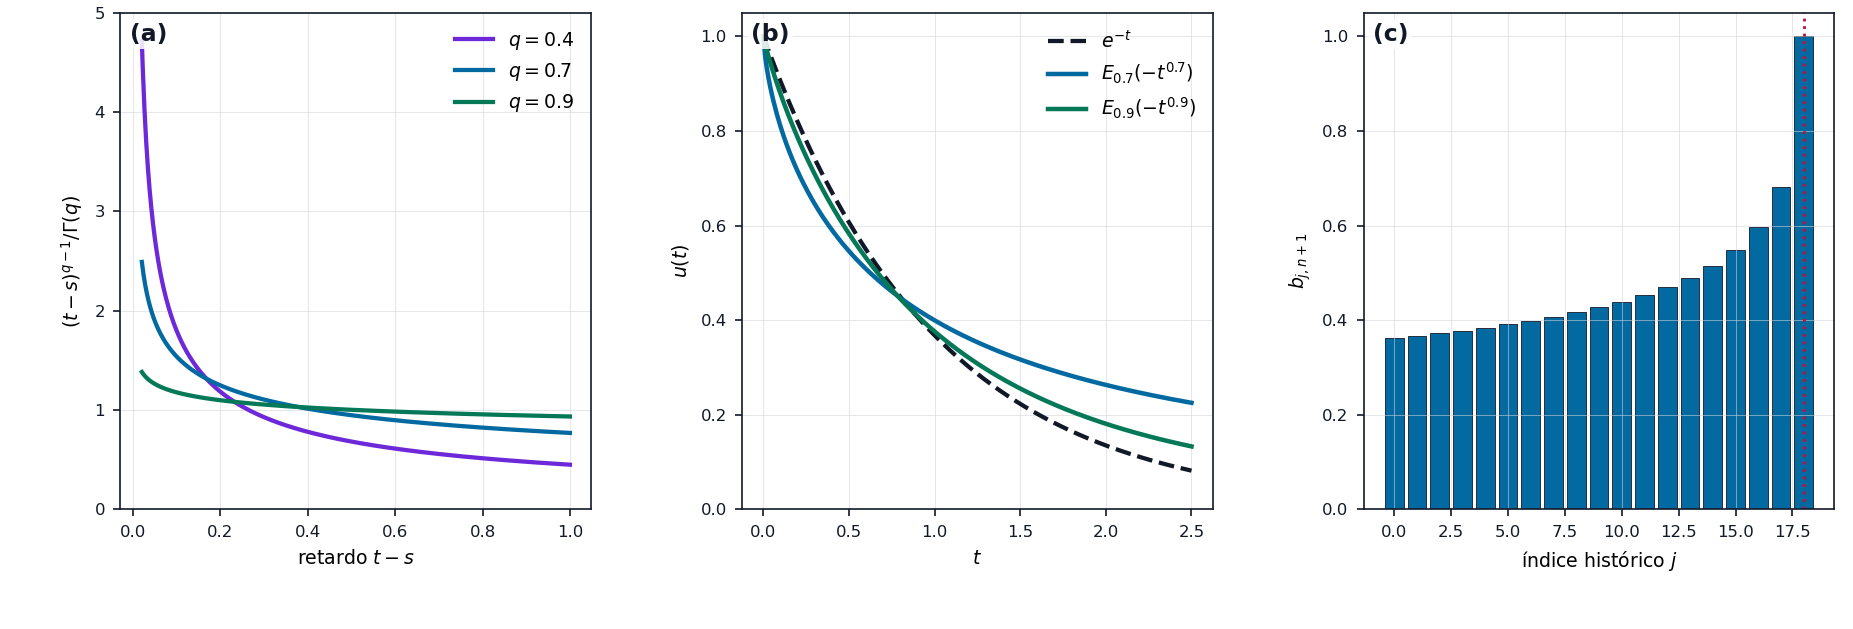
\includegraphics[width=0.94\linewidth]{fractional_memory_kernel_pece.png}
\caption{Tres superficies de lectura para un problema de Caputo: (a) kernel de
memoria para varios órdenes, (b) relajación de Mittag--Leffler comparada con el caso
exponencial y (c) pesos históricos del predictor ABM. La altura de un peso representa una
contribución que debe multiplicarse por la evaluación histórica correspondiente y sumarse
desde el terminal inferior fijo.}
\label{fig:gt-memoria-abm}
\end{figure}

\begin{activitybox}{Laboratorio numérico: relajación escalar}
Implemente \eqref{eq:gt-abm-predictor}--\eqref{eq:gt-abm-pesos} para
${}^{\mathrm C}D^qx=-x$, $x(0)=1$, $q=0.8$, $T=5$ y
$h=0.05,0.025,0.0125$. Compare con $E_q(-t^q)$ y reporte el error máximo en una
malla común. Como control dentro de Toolbox Chaos, defina $\dot x=-x$ en
\gui{Crear sistema} y compare Euler, Heun y RK4 mediante \gui{Comparar metodos}:
esta ejecución corresponde al límite entero; el cálculo con memoria conserva el historial completo.
Conserve tabla, configuración y una gráfica de error; no entregue únicamente curvas
superpuestas.
\end{activitybox}

\begin{warningbox}
Un método que reinicia periódicamente desde el último valor de $x$ no implementa la
misma ecuación de Caputo con terminal inferior fijo. Una coincidencia visual durante
un intervalo corto no corrige esa diferencia. Antes de comparar dos soluciones deben
coincidir operador, orden, terminal inferior, historia, política de memoria, paso y
horizonte.
\end{warningbox}

\lecturaseccion{Kai Diethelm, \emph{The Analysis of Fractional Differential
Equations}, sección del método predictor--corrector; K. Diethelm, N. J. Ford y A. D.
Freed, ``A predictor-corrector approach for the numerical solution of fractional
differential equations'', \emph{Nonlinear Dynamics}, 2002; Igor Podlubny,
\emph{Fractional Differential Equations}, secciones numéricas.}

\subsection{Comprobación de hipótesis y resultados}

Los conceptos anteriores forman una cadena, no una colección de palabras. El espacio
de fases fija qué estados y vecindades son legítimos. La existencia y unicidad
permiten hablar de flujo. La invariancia y las regiones atrapantes organizan el
comportamiento global. La variación describe perturbaciones; Poincaré convierte un
ciclo en un punto fijo; Floquet mide su estabilidad transversal. El grado responde
preguntas de existencia sin resolver necesariamente el objeto. Las intersecciones de
variedades conectan geometría con dinámica simbólica. En Caputo, toda la cadena debe
levantarse a un estado que conserve memoria.

\begin{longtable}{>{\raggedright\arraybackslash}p{0.19\linewidth}
                  >{\raggedright\arraybackslash}p{0.34\linewidth}
                  >{\raggedright\arraybackslash}p{0.37\linewidth}}
\toprule
Objeto & Pregunta matemática & Comprobación antes de interpretar una gráfica\\
\midrule
\endhead
Espacio de fases & ¿Qué representa un estado y qué puntos se identifican? & Unidades,
periodicidad angular, dimensión y distancia elegida.\\
Flujo & ¿Existe una evolución única y componible? & Regularidad del campo, intervalo
de existencia y dependencia de la condición inicial.\\
Invariancia & ¿Las trayectorias permanecen en el conjunto? & Signo del campo en la
frontera o argumento exacto de conservación.\\
Atracción & ¿La distancia al conjunto tiende a cero? & Varias condiciones iniciales,
transitorio, horizonte y definición de distancia.\\
Variedad estable & ¿Qué estados convergen al objeto hiperbólico? & Espectro local,
tangencia y continuidad al ampliar la integración.\\
Retorno & ¿El siguiente cruce define una función? & Sección, orientación, exclusión de
tangencias e interpolación del evento.\\
Floquet & ¿Cómo cambia una perturbación después de un periodo? & Periodo, integración
variacional, multiplicador trivial y convergencia numérica.\\
Grado & ¿Debe existir un cero o punto fijo dentro de la región? & Ausencia de ceros en
la frontera y continuidad durante la homotopía.\\
Dinámica simbólica & ¿Existe una codificación compatible con la iteración? & Región
invariante, partición, cobertura y correspondencia de itinerarios.\\
Memoria Caputo & ¿Qué historia determina la continuación? & Orden, terminal inferior,
perfil, política de memoria y comparación de pasos.\\
\bottomrule
\end{longtable}

\begin{activitybox}{Proyecto breve: una afirmación, tres niveles de evidencia}
Elija uno de estos objetos: región atrapante de \eqref{eq:gt-normal-radial}, variedad
de \eqref{eq:gt-silla-no-lineal}, retorno del ciclo radial o itinerarios del mapa
logístico. Entregue una página con: definición; derivación analítica; experimento en
Toolbox Chaos; dos refinamientos; interpretación de cada gráfica; y una frase precisa
sobre el alcance que ya se estableció. Otra persona debe poder repetir el cálculo con
la información escrita, sin instrucciones orales.
\end{activitybox}

\paragraph{Problemas de cierre.}
\begin{enumerate}
  \item Demuestre que la imagen de un conjunto conexo bajo una aplicación continua es
  conexa. Explique cómo usaría el resultado para revisar una transformación de
  coordenadas.
  \item Para $\dot x=x(1-x)$, determine flujo implícito, equilibrios, cuencas y
  conjuntos $\omega$-límite. Dibuje primero la línea de fase.
  \item Construya una función $h$ cuya subnivel describa un disco y aplique
  \eqref{eq:gt-derivada-lie} al sistema radial.
  \item Verifique \eqref{eq:gt-liouville} para un sistema lineal diagonal y compare
  con el producto de sus soluciones escalares.
  \item En \eqref{eq:gt-silla-no-lineal}, busque el siguiente término de una gráfica
  invariante $h(x)=a_2x^2+a_3x^3$ y explique por qué $a_3=0$.
  \item Derive \eqref{eq:gt-multiplicador-planar} a partir de
  \eqref{eq:gt-liouville} y del multiplicador tangencial igual a uno.
  \item Para $P(x)=rx(1-x)$, determine la estabilidad de los puntos fijos y describa
  qué cambia cuando un multiplicador cruza $-1$.
  \item Justifique por qué un grado no nulo de $P-I$ demuestra existencia de un punto
  fijo, pero no su estabilidad.
  \item Compare recurrencia en el estado puntual con recurrencia del perfil
  $m_t(\theta)$ de \eqref{eq:gt-perfil-memoria}.
  \item Pruebe que los pesos $b_{j,n+1}$ de
  \eqref{eq:gt-abm-predictor} son positivos y explique su comportamiento para datos
  muy antiguos.
\end{enumerate}

\paragraph{Criterios de resolución para los problemas 1--10.}
En el problema 1 use la caracterización de conexidad por separaciones. En el 2 separe
variables y conserve los signos antes de integrar. En el 3 tome
$h=x^2+y^2-R^2$. En el 4 use
$M(t)=\operatorname{diag}(e^{\lambda_1t},\ldots,e^{\lambda_nt})$. En el 5 sustituya
la serie en \eqref{eq:gt-invariancia-grafica}. En el 6 separe la dirección tangente de
la transversal. En el 7 derive $P'(x^*)$. En el 8 recuerde que el grado no contiene
tasas temporales. En el 9 construya dos perfiles con el mismo valor en cero. En el 10
use que $u^q$ es creciente para $q>0$.

\begin{evidencebox}{Criterio de avance}
El capítulo está dominado cuando puede explicarse a partir de definiciones y teoremas por qué una
frontera de píxeles requiere una definición de frontera matemática; la linealización es
local; cómo un ciclo se convierte en punto fijo de retorno; qué aporta un grado no
nulo; qué hipótesis geométrica precede a una herradura; y por qué en Caputo el valor
actual requiere la historia necesaria para continuar.
\end{evidencebox}


% Profundización y proyecto. Se incluye desde manual_teorico_pedagogico.tex.

\section{Mapas, flujos, señales y sistemas avanzados}

\begin{objectivebox}
Integrar teoría y cómputo para estudiar mapas discretos, flujos caóticos canónicos,
rutas al caos, geometría fractal, datos temporales, retardo, alta dimensión,
dinámica conservativa y transitoria, sincronización, control y memoria fraccionaria.
La meta es formular conclusiones graduadas: qué se derivó, qué se observó, qué
indicador se estimó y qué permanece abierto.
\end{objectivebox}

\subsection{Mapa logístico y diagrama de telaraña}

\paragraph{Ecuación del mapa logístico.}
Un \term{mapa dinámico} actualiza el estado en instantes discretos:
\[
 x_{n+1}=f(x_n;\mu).
\]
La órbita de \(x_0\) es la sucesión
\(\{x_0,f(x_0),f^2(x_0),\ldots\}\). Un punto fijo satisface
\(f(x^*)=x^*\); un punto de periodo primo \(p\) satisface
\(f^p(x)=x\) y no vuelve antes. Para un punto fijo hiperbólico,
\[
 |f'(x^*)|<1\quad\Longrightarrow\quad\text{atractor local},\qquad
 |f'(x^*)|>1\quad\Longrightarrow\quad\text{repulsor local}.
\]
La derivada es un \term{multiplicador por iteración}; las tasas por unidad de tiempo corresponden a los flujos continuos.

\paragraph{Construcción de telaraña.}
En el plano \((x_n,x_{n+1})\), se dibujan \(y=f(x)\) y la diagonal \(y=x\).
Desde \(x_n\), un segmento vertical llega a \(f(x_n)\) y uno horizontal regresa a la
diagonal, donde queda \(x_{n+1}\). La alternancia reproduce exactamente la iteración;
representa la actualización discreta del mapa. Una convergencia alternante indica multiplicador negativo,
mientras que una convergencia sin alternancia suele asociarse con uno positivo.

\paragraph{Ejemplo algebraico resuelto: mapa logístico.}
Para
\[
 f_r(x)=rx(1-x),\qquad 0\leq x\leq1,
\]
los puntos fijos satisfacen
\[
 x=rx(1-x)\quad\Longrightarrow\quad
 x_0^*=0,\qquad x_1^*=1-\frac1r\quad(r\ne0).
\]
Como \(f_r'(x)=r(1-2x)\),
\[
 f_r'(0)=r,\qquad
 f_r'(x_1^*)=2-r.
\]
El origen es estable para \(|r|<1\); el punto no nulo es estable cuando
\(|2-r|<1\), es decir, \(1<r<3\). En \(r=3\) su multiplicador cruza \(-1\), firma
local de la primera duplicación de periodo.

Para \(r=4\) y \(x_0=0.2\),
\[
 x_1=0.64,\qquad x_2=0.9216,\qquad
 x_3=4(0.9216)(0.0784)=0.28901376.
\]
Los tres valores son reproducibles a mano; la interpretación requiere el cálculo de
indicadores además de la apariencia de la gráfica. El exponente finito de una órbita se estima mediante
\[
 \lambda_N=\frac1N\sum_{n=0}^{N-1}
 \log|r(1-2x_n)|.
\]

\begin{activitybox}{Práctica reproducible: cuatro regímenes logísticos}
Seleccione el sistema logístico registrado o defínalo como mapa en
\gui{Crear sistema}. Use \(x_0=0.2\), descarte 500 iteraciones y conserve 500.
Ejecute \(r=2.8\), \(3.2\), \(3.5\) y \(4\). Para los dos primeros dibuje a mano
las primeras veinte etapas de la telaraña; para todos exporte la serie y calcule
\(\lambda_N\). En \gui{Bifurcación}, barra \(r\in[2.5,4]\) con una malla que después
duplique. Conserve el mismo transitorio y número de muestras al comparar.
\end{activitybox}

\begin{figure}[H]
\centering
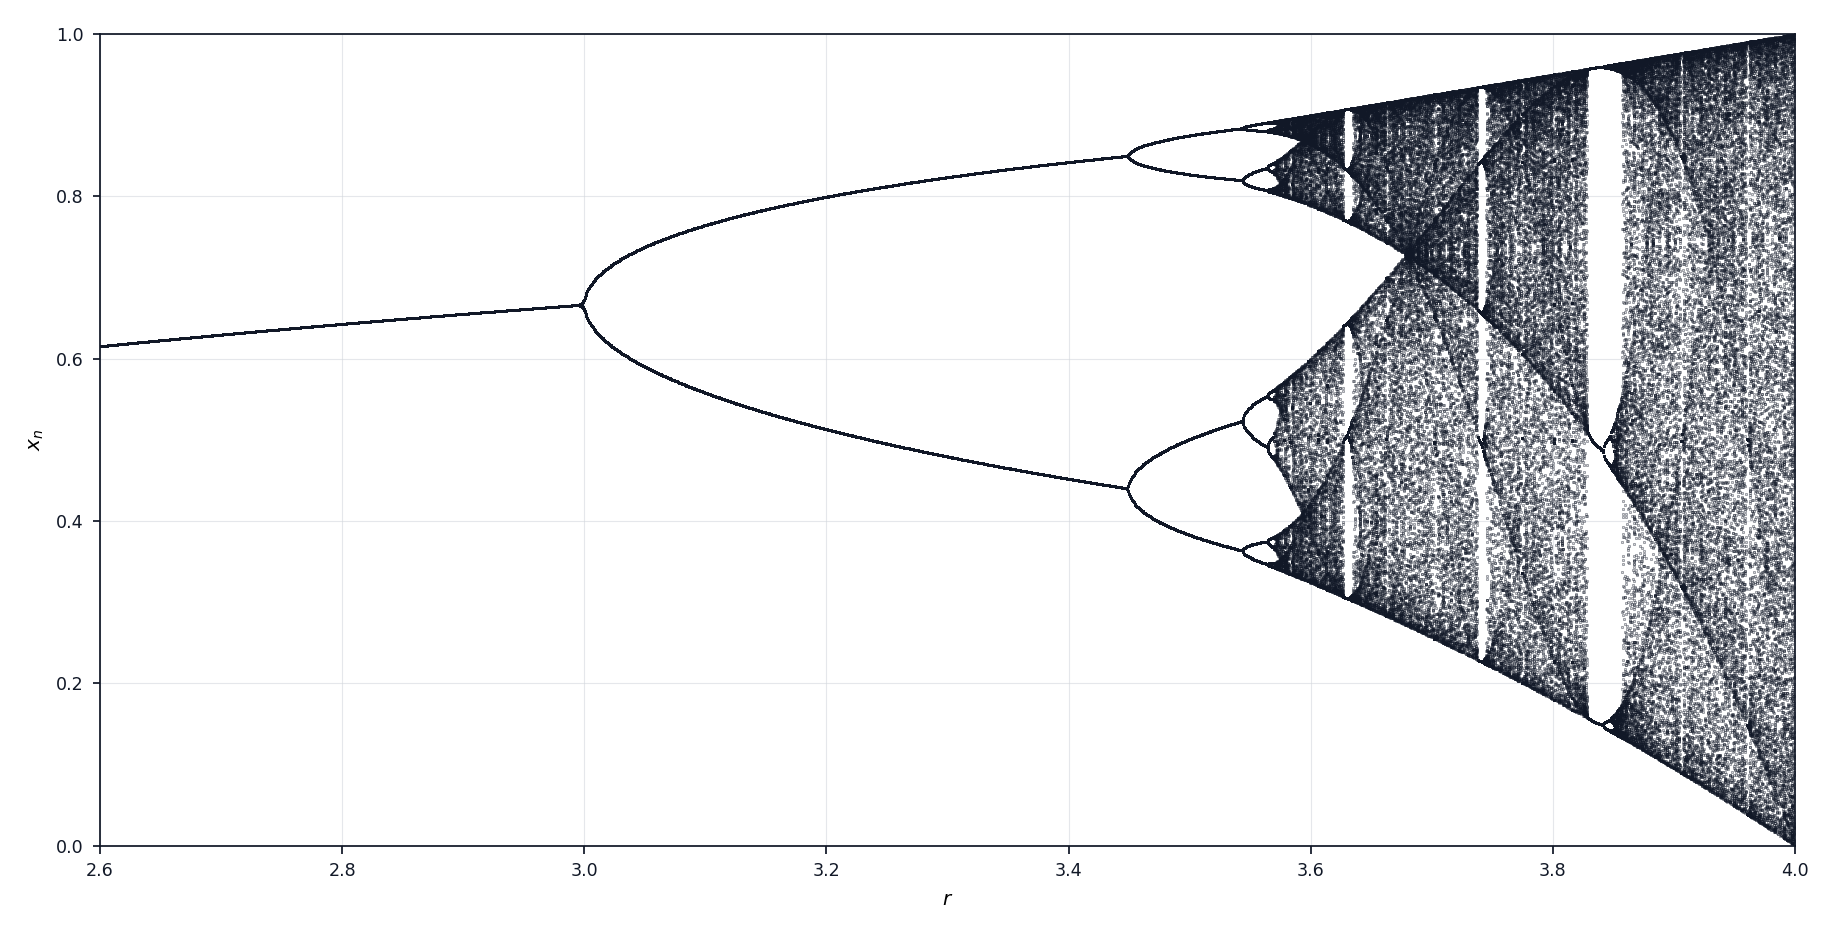
\includegraphics[width=0.86\linewidth]{logistic_bifurcation.png}
\caption{Diagrama logístico producido para el manual con el software. Cada columna
contiene iterados tardíos para un parámetro; las líneas aparentes son conjuntos de
puntos muestreados, no curvas de soluciones continuas.}
\label{fig:logistica-profundizacion}
\end{figure}

\paragraph{Lectura de la órbita logística.}
Una rama única corresponde a un valor tardío dominante; dos ramas, a una órbita de
periodo dos, si se confirma el orden temporal. Una banda densa puede contener órbitas
caóticas, inestables, preperiódicas y efectos de resolución. Las ventanas claras
dentro de bandas densas motivan una simulación local con mayor transitorio.

\begin{warningbox}
El diagrama de bifurcación debe leerse junto con \(x_0\), transitorio, aritmética, malla y dirección del barrido. La identificación de un atractor único exige
telaraña con muchas líneas tampoco demuestra sensibilidad; para ello se comparan
órbitas vecinas o se estima expansión con control de convergencia.
\end{warningbox}

\lecturaseccion{Steven H. Strogatz, \emph{Nonlinear Dynamics and Chaos with
Applications to Physics, Biology, Chemistry, and Engineering},
2.\textsuperscript{a} ed., secciones 10.1, ``Fixed Points and Cobwebs'', 10.2--10.5,
sobre mapa logístico, ventanas y exponente de Lyapunov; Robert L. Devaney,
\emph{A First Course in Chaotic Dynamical Systems: Theory and Experiment},
2.\textsuperscript{a} ed., capítulos 4--8, sobre análisis gráfico, puntos fijos,
bifurcaciones y diagrama de órbitas; Kathleen T. Alligood, Tim D. Sauer y James A.
Yorke, \emph{Chaos: An Introduction to Dynamical Systems}, secciones 1.1--1.7.}

\subsection{Mapa de Hénon, plegamiento y dinámica simbólica}

\paragraph{Ecuaciones y puntos fijos de Hénon.}
Un mapa bidimensional puede contraer área en una dirección y estirar y plegar en
otra. El mapa de Hénon, en una convención habitual, es
\[
 x_{n+1}=1-a x_n^2+y_n,\qquad y_{n+1}=b x_n.
\]
Su Jacobiano es
\[
 DF(x,y)=
 \begin{pmatrix}-2ax&1\\ b&0\end{pmatrix},\qquad
 \det DF=-b.
\]
Por tanto, un elemento de área cambia su magnitud por el factor constante \(|b|\).
Con \(|b|<1\) existe contracción de área. La clasificación de cada órbita requiere
acotada.

La \term{dinámica simbólica} asigna a cada estado un símbolo según una partición. Un
itinerario \(s_0s_1s_2\cdots\) registra qué región visita la órbita. Para que esta
codificación sea una representación matemática completa se necesita justificar una
partición generadora y una relación con un desplazamiento simbólico; etiquetar puntos
por su signo sólo produce un resumen.

\paragraph{Ejemplo algebraico resuelto: puntos fijos de Hénon.}
En un punto fijo \(y^*=bx^*\) y
\[
 x^*=1-a(x^*)^2+bx^*,
\]
de modo que
\[
 a(x^*)^2+(1-b)x^*-1=0.
\]
Para \(a=1.4\), \(b=0.3\),
\[
 x_\pm^*=\frac{-0.7\pm\sqrt{6.09}}{2.8}
 \simeq 0.63135,\ -1.13135,
\qquad y_\pm^*=0.3x_\pm^*.
\]
En cada punto, \(\tau=-2ax^*\) y \(\Delta=-0.3<0\). Por el criterio plano, ambos
son sillas. El atractor numérico clásico, cuando se observa, pertenece a la dinámica alejada de esos puntos;
su organización está vinculada con las variedades de las sillas y el plegamiento
global.

\paragraph{Itinerario simbólico del mapa de Hénon.}
Defina \(s_n=L\) si \(x_n<0\) y \(s_n=R\) si \(x_n\geq0\). La palabra
\(RRL LR\), sin espacios, identifica cinco visitas, pero no conserva amplitudes ni
distancias. Las frecuencias de bloques \(LR\), \(RL\), \(LL\), \(RR\) pueden comparar
órbitas largas; la condición de bloque prohibido requiere muestras y criterios adicionales.

\begin{activitybox}{Práctica reproducible: Hénon y un alfabeto binario}
Genere Hénon con \(a=1.4\), \(b=0.3\), \((x_0,y_0)=(0,0)\), 20000 iteraciones y
descarte 2000. Use \gui{Series temporales} y \gui{Retratos 2D}; exporte los datos.
Verifique los dos puntos fijos calculados y clasifíquelos con sus matrices. Codifique
las últimas 10000 observaciones mediante \(L/R\), cuente bloques de longitud dos y
tres y repita con \((10^{-8},0)\). Registre si cambian las frecuencias dentro de la
precisión muestral.
\end{activitybox}

\begin{figure}[H]
\centering
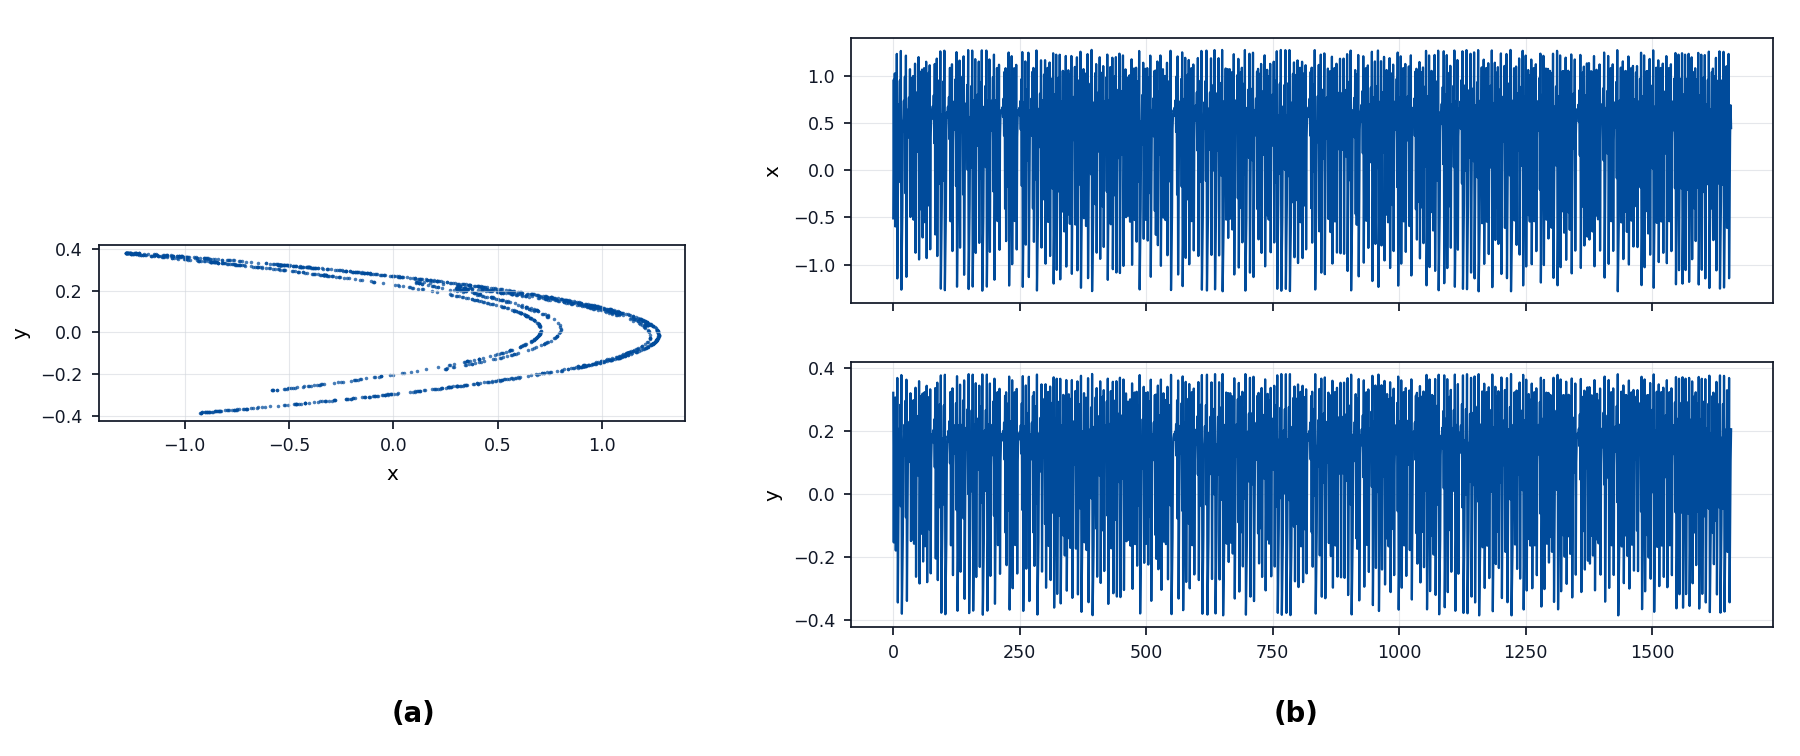
\includegraphics[width=0.82\linewidth]{systems/henon_phase_timeseries.png}
\caption{Retrato y serie del mapa de Hénon generados por Toolbox Chaos. El retrato
revela plegamiento geométrico; la serie conserva el orden de visitas que se pierde en
la nube plana.}
\label{fig:henon-profundizacion}
\end{figure}

\paragraph{Lectura del retrato de fase de Hénon.}
El espesor aparente del conjunto depende de resolución, antialiasing y número de
puntos. Una ampliación debe recalcular o redibujar los datos, no ampliar una captura.
La serie permite detectar escape o periodicidad; el retrato revela foliaciones y
plegamiento; el itinerario simbólico resume recurrencia entre regiones.

\begin{warningbox}
\(|\det DF|<1\) demuestra contracción local de área. La existencia y unicidad de un
atractor, la sensibilidad y la conjugación con el desplazamiento de Bernoulli requieren verificar hipótesis adicionales sobre la partición y los itinerarios.
\end{warningbox}

\lecturaseccion{Steven H. Strogatz, \emph{Nonlinear Dynamics and Chaos with
Applications to Physics, Biology, Chemistry, and Engineering},
2.\textsuperscript{a} ed., sección 12.2, ``The Hénon Map''; Kathleen T. Alligood,
Tim D. Sauer y James A. Yorke, \emph{Chaos: An Introduction to Dynamical Systems},
secciones 2.2, 2.5--2.6, 3.5 y 5.6; Robert L. Devaney,
\emph{A First Course in Chaotic Dynamical Systems: Theory and Experiment},
2.\textsuperscript{a} ed., capítulo 9, sobre dinámica simbólica, desplazamiento y
conjugación; Morris W. Hirsch, Stephen Smale y Robert L. Devaney,
\emph{Differential Equations, Dynamical Systems, and an Introduction to Chaos},
3.\textsuperscript{a} ed., capítulo 15, apartados sobre caos, dinámica simbólica,
desplazamiento y conjunto de Cantor.}

\subsection{Lorenz, Rössler, Chua y Duffing--Ueda}

\paragraph{Mecanismos dinámicos en cuatro modelos.}
Estos sistemas son laboratorios matemáticos, no plantillas intercambiables. Lorenz
combina convección idealizada, simetría y disipación:
\[
 \dot x=\sigma(y-x),\qquad
 \dot y=x(\rho-z)-y,\qquad
 \dot z=xy-\beta z.
\]
Rössler concentra la no linealidad en una ecuación:
\[
 \dot x=-y-z,\qquad
 \dot y=x+ay,\qquad
 \dot z=b+z(x-c).
\]
Una forma de Chua usa una no linealidad por tramos:
\[
 \dot x=\alpha[y-x-h(x)],\quad
 \dot y=x-y+z,\quad
 \dot z=-\beta y,
\]
\[
 h(x)=m_1x+\frac{m_0-m_1}{2}
 \bigl(|x+1|-|x-1|\bigr).
\]
Duffing--Ueda es no autónomo; con la fase del forzamiento se escribe
\[
 \dot x=v,\quad
 \dot v=-2\zeta v-x-sx^3+f\cos\phi,\quad
 \dot\phi=\nu.
\]

\paragraph{Ejemplo algebraico resuelto: Lorenz clásico.}
La divergencia del campo es constante:
\[
 \nabla\cdot\mathbf f=-\sigma-1-\beta.
\]
Para \((\sigma,\rho,\beta)=(10,28,8/3)\) vale \(-41/3<0\); un volumen infinitesimal
se contrae como \(\exp[-(41/3)t]\). Esto demuestra disipación volumétrica local, no
acotación global por sí sola.

Los equilibrios son
\[
 E_0=(0,0,0),\qquad
 E_\pm=\bigl(\pm\sqrt{\beta(\rho-1)},
             \pm\sqrt{\beta(\rho-1)},\rho-1\bigr)
\]
cuando \(\rho>1\). En el caso clásico,
\[
 E_\pm=(\pm6\sqrt2,\pm6\sqrt2,27).
\]
La transformación \((x,y,z)\mapsto(-x,-y,z)\) deja invariantes las ecuaciones y
explica la simetría de los dos lóbulos. No obliga a una trayectoria finita a pasar
exactamente el mismo tiempo en cada uno.

\paragraph{Estructura algebraica de los cuatro modelos.}
En Rössler,
\[
 \nabla\cdot\mathbf f=a+x-c,
\]
que varía a lo largo de la órbita; en el Duffing autónomo,
\(\nabla\cdot\mathbf f=-2\zeta\). En Chua, la pendiente efectiva de \(h(x)\) cambia
al cruzar los quiebres. Por tanto, ``disipativo'' puede significar contracción
instantánea constante, contracción media o contracción por regiones; el cálculo debe
acompañar la etiqueta.

\begin{activitybox}{Práctica reproducible: atlas de cuatro flujos}
En cada pestaña seleccione el preset registrado de Lorenz, Rössler, Chua y
Duffing--Ueda. Antes de ejecutar copie las ecuaciones, parámetros y estado inicial que
muestra la interfaz. Use RK4 y el paso recomendado por cada preset; genere
\gui{Atractor 3D}, pulse \gui{Usar última trayectoria} en \gui{Retratos 2D} y
\gui{Series temporales}, y repita con la mitad del paso y el mismo horizonte físico.
Para Lorenz marque \(E_0,E_\pm\). Para Duffing interprete la fase como reloj del
forzamiento y construya, desde los datos, una sección cada \(2\pi/\nu\).
\end{activitybox}

\begin{figure}[H]
\centering
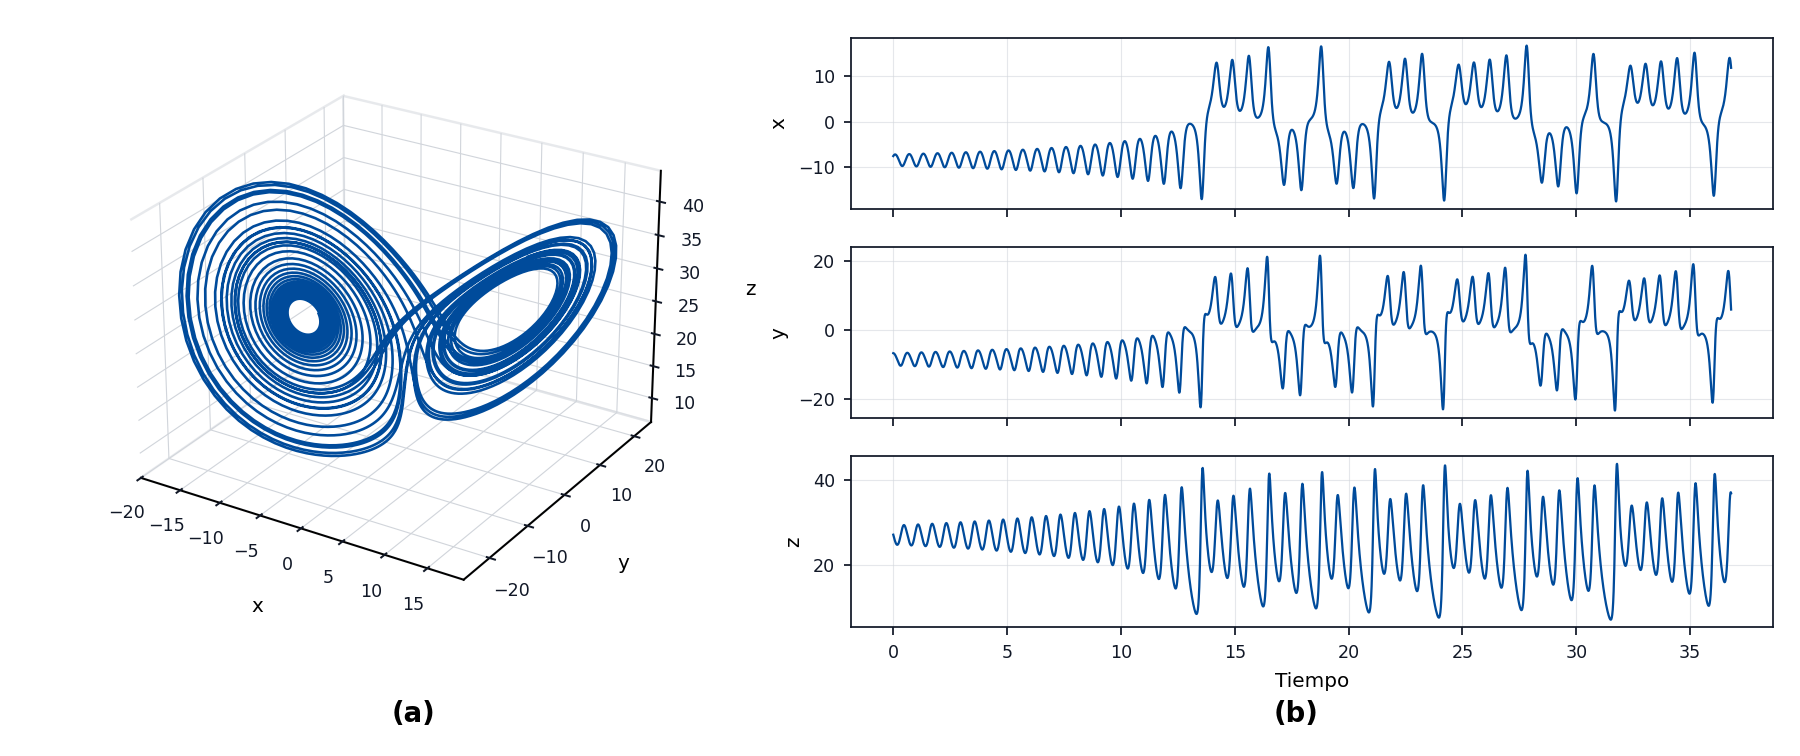
\includegraphics[width=0.90\linewidth]{systems/lorenz_phase_timeseries.png}
\caption{Lorenz en una vista combinada de trayectoria y series generada por Toolbox
Chaos. Los lóbulos reflejan la simetría del campo; los cambios de lóbulo se localizan
mejor al conservar el orden temporal.}
\label{fig:software-lorenz}
\end{figure}

\begin{figure}[H]
\centering
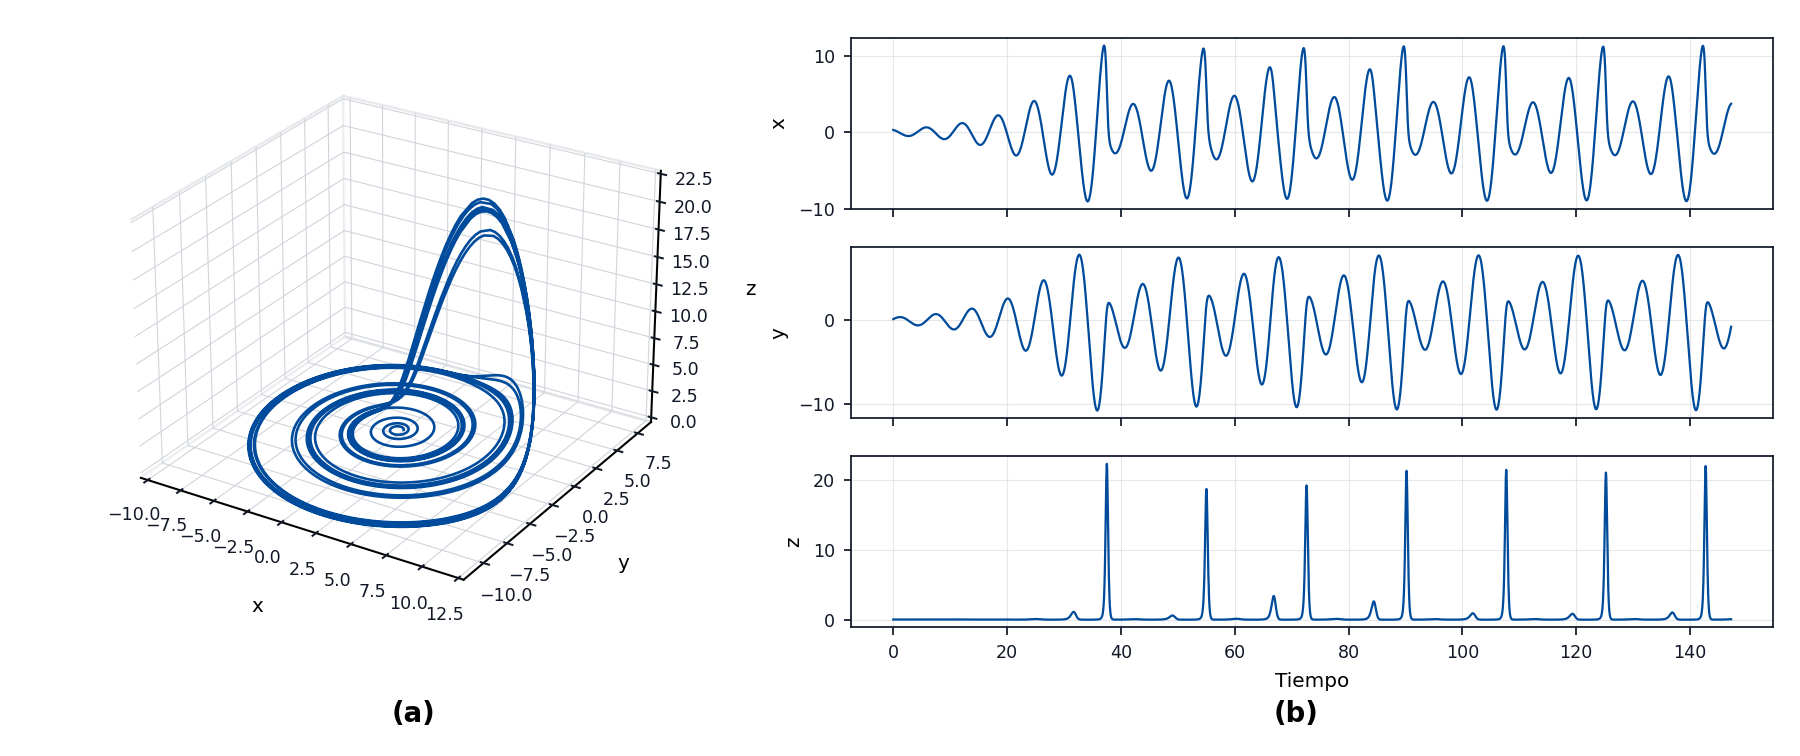
\includegraphics[width=0.90\linewidth]{systems/rossler_phase_timeseries.png}
\caption{Rössler generado por Toolbox Chaos. La rotación casi plana y las excursiones
en la tercera coordenada sugieren un mecanismo de estiramiento y reinyección; la
proyección requiere el procedimiento adicional que establece una sección de retorno unimodal.}
\label{fig:software-rossler}
\end{figure}

\begin{figure}[H]
\centering
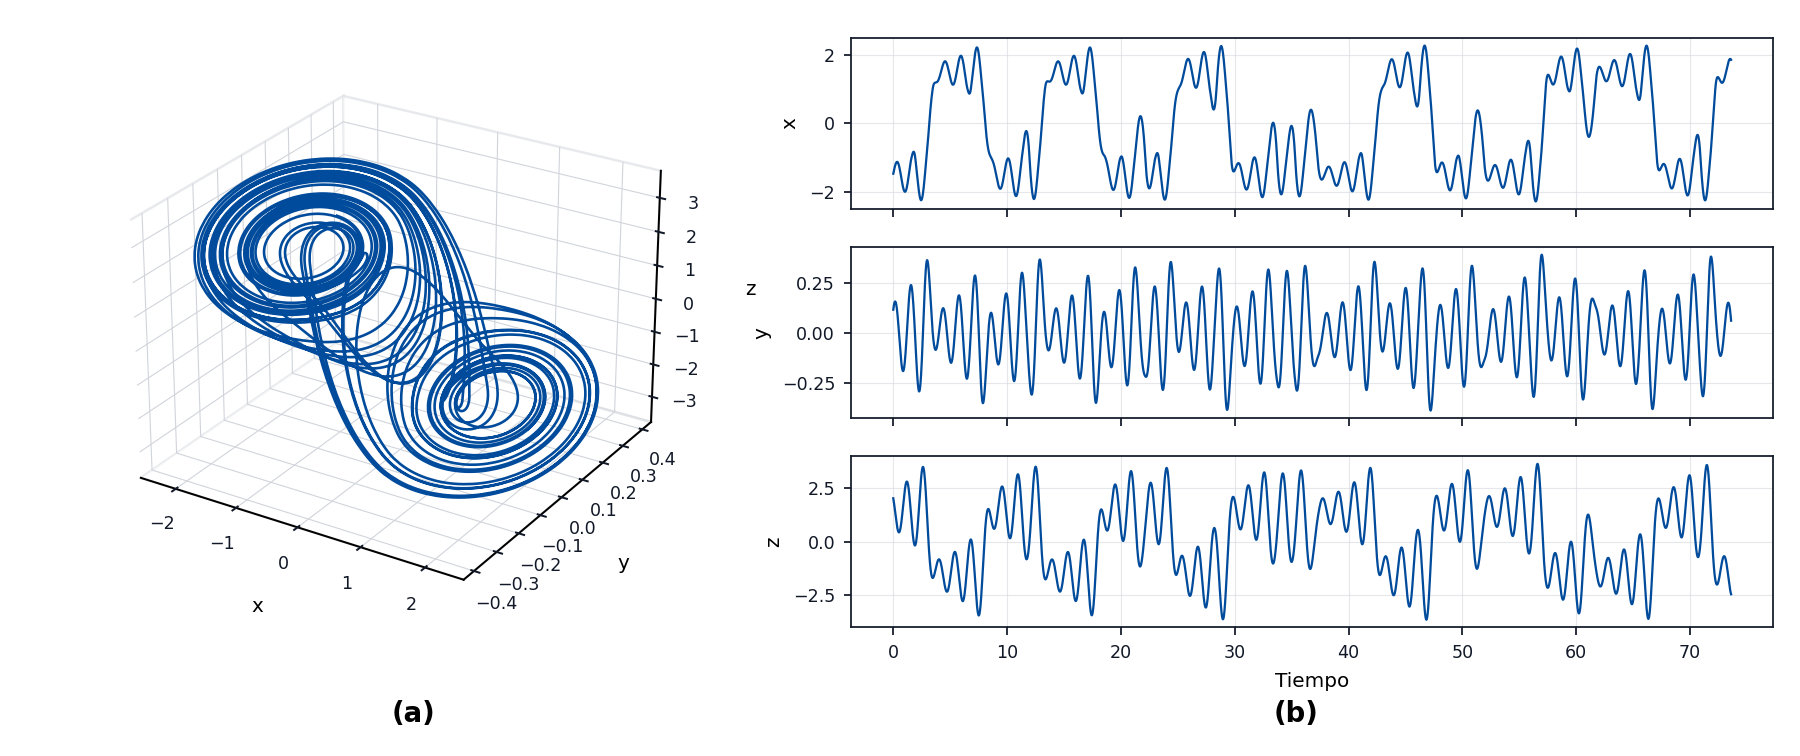
\includegraphics[width=0.90\linewidth]{systems/chua_phase_timeseries.png}
\caption{Chua generado por Toolbox Chaos. Los cambios entre regiones de la
característica por tramos organizan la geometría de doble desplazamiento; los quiebres
de la ecuación deben interpretarse junto con la escala de los ejes.}
\label{fig:software-chua}
\end{figure}

\begin{figure}[H]
\centering
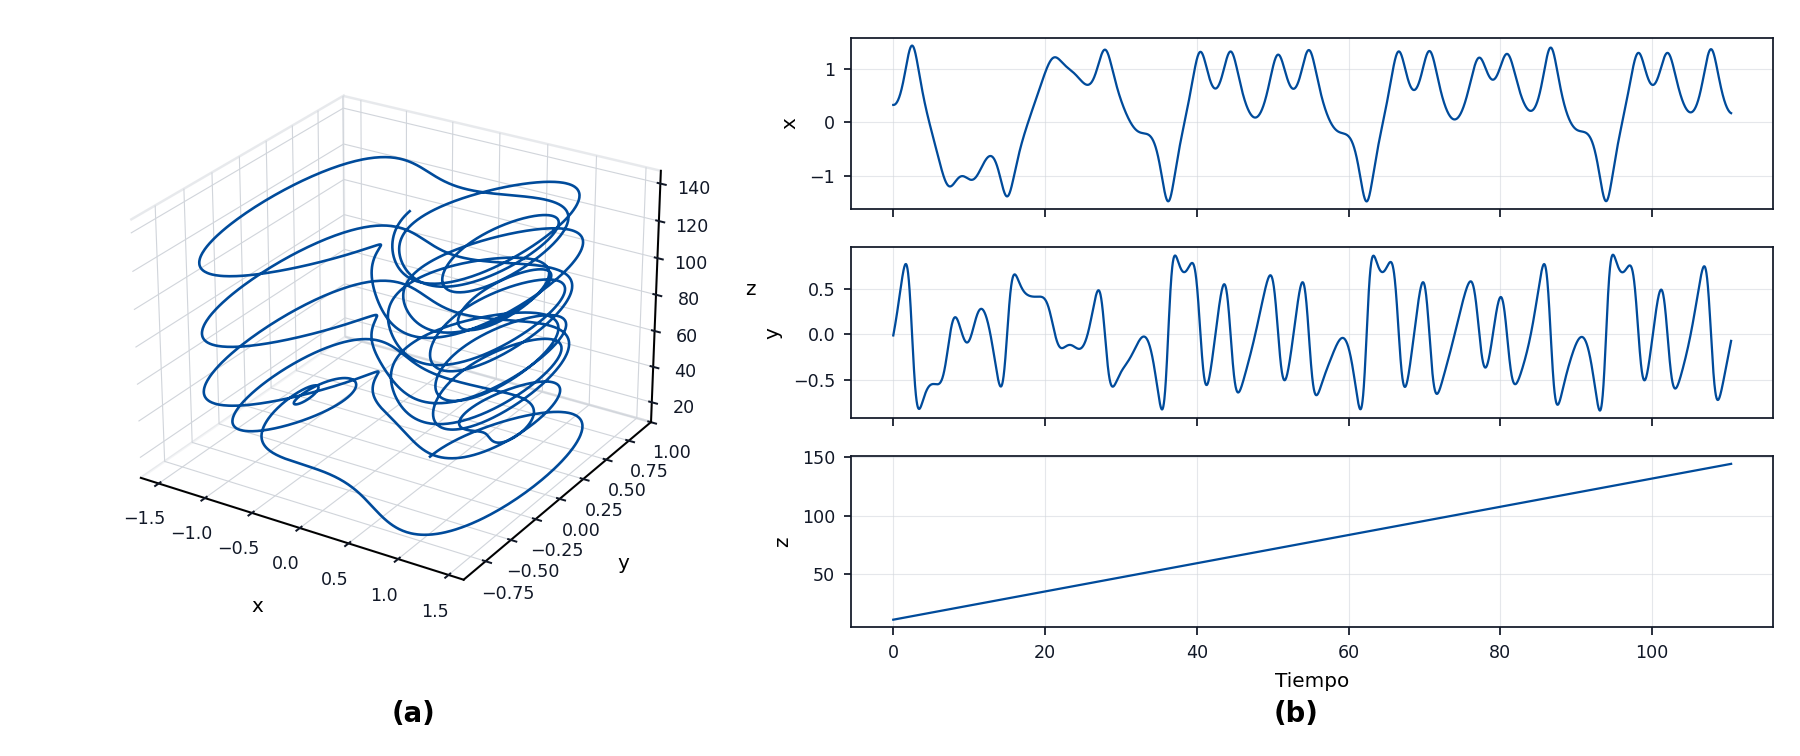
\includegraphics[width=0.90\linewidth]{systems/duffing_ueda_phase_timeseries.png}
\caption{Duffing--Ueda generado por Toolbox Chaos. El retrato proyectado mezcla
movimiento y fase de forzamiento; una sección estroboscópica separa mejor periodicidad,
cuasiperiodicidad y respuesta irregular.}
\label{fig:software-duffing}
\end{figure}

\paragraph{Variables para analizar cada modelo.}
En cada figura identifique: variable horizontal y vertical; tramo transitorio; rango
tardío; simetrías; vecindad de equilibrios; orientación; frecuencia de retornos; y
posibles saturaciones. Después formule una frase causal vinculada con un término de
la ecuación y una frase prudente que describa sólo lo observado. Esta doble redacción
evita que un parecido visual sustituya el análisis.

\begin{warningbox}
Las cuatro imágenes fueron generadas con configuraciones concretas del software. No
son retratos de todo el espacio de parámetros. La identificación de Lorenz, Rössler y caos en Chua requiere contrastar los retratos con ecuaciones y diagnósticos; una respuesta irregular de Duffing requiere controlar transitorios y aliasing.
\end{warningbox}

\lecturaseccion{Julien C. Sprott, \emph{Elegant Chaos: Algebraically Simple Chaotic
Flows}, capítulo 2, apartados sobre van der Pol, Rayleigh y Duffing forzados, y
capítulo 3, apartados sobre Lorenz, Rössler, sistemas de Sprott, ecuaciones jerk y
Chua; Kathleen T. Alligood, Tim D. Sauer y James A. Yorke,
\emph{Chaos: An Introduction to Dynamical Systems}, capítulo 9, apartados sobre
Lorenz, Rössler, Chua, flujos forzados y exponentes de Lyapunov; Morris W. Hirsch,
Stephen Smale y Robert L. Devaney, \emph{Differential Equations, Dynamical Systems,
and an Introduction to Chaos}, 3.\textsuperscript{a} ed., capítulos 14 y 16,
apartados sobre Lorenz, Rössler, doble desplazamiento y circuito de Chua.}

\subsection{Rutas al caos: duplicación, cuasiperiodicidad, intermitencia y crisis}

\paragraph{Mecanismos de transición al caos.}
Una \term{ruta al caos} es una secuencia organizada de cambios al variar un
parámetro. Entre las rutas frecuentes se encuentran:
\begin{itemize}
  \item duplicaciones sucesivas del periodo;
  \item ruptura de un toro después de movimiento cuasiperiódico;
  \item intermitencia, con fases casi regulares interrumpidas por ráfagas;
  \item crisis, donde una colisión global cambia bruscamente tamaño, acceso o vida de
  un conjunto caótico;
  \item bifurcaciones homoclínicas o heteroclínicas asociadas con variedades
  invariantes.
\end{itemize}
Estas etiquetas requieren evidencias diferentes. Un diagrama de máximos es eficaz
para duplicación y crisis; un número de rotación y espectro son más informativos para
cuasiperiodicidad; una distribución de longitudes laminares ayuda en intermitencia.

\paragraph{Ejemplo algebraico resuelto: primera cascada logística.}
La rama fija no nula del mapa logístico tiene multiplicador \(2-r\), que alcanza
\(-1\) en \(r=3\). Los puntos de periodo dos que no son fijos son
\[
 x_\pm=\frac{r+1\pm\sqrt{(r-3)(r+1)}}{2r}.
\]
Para \(r=3.2\),
\[
 x_-\simeq0.5130,\qquad x_+\simeq0.7995.
\]
El multiplicador del ciclo es el producto
\[
 M_2=f'(x_-)f'(x_+)=-r^2+2r+4.
\]
En \(r=3.2\), \(M_2=0.16\), por lo que el ciclo es estable. Pierde estabilidad
cuando \(M_2=-1\), es decir, en \(r=1+\sqrt6\simeq3.44949\). Este cálculo localiza
dos niveles de la cascada sin depender de la resolución del diagrama.

\paragraph{Escalamiento de Feigenbaum.}
Si \(r_n\) son parámetros de duplicaciones sucesivas en una familia unimodal
genérica, las razones
\[
 \delta_n=\frac{r_{n-1}-r_{n-2}}{r_n-r_{n-1}}
\]
pueden aproximarse a una constante universal. La universalidad requiere hipótesis
sobre la familia y un límite; una razón calculada con tres puntos aproximados no la
demuestra.

\begin{activitybox}{Práctica reproducible: distinguir cuatro rutas}
Primero use \gui{Bifurcación} para la logística y refine los intervalos alrededor de
\(r=3\) y \(r=1+\sqrt6\). Después, con Duffing--Ueda, construya secciones
estroboscópicas para una secuencia de amplitudes de forzamiento tomada del preset y
registre si aparece un número finito de puntos, una curva o una nube. Para Lorenz,
barra \(\rho\) en ambas direcciones y use el mismo estado inicial y transitorio.
Cuando observe un salto, simule a ambos lados con horizontes duplicados y varias
condiciones iniciales.
\end{activitybox}

\paragraph{Lectura de las rutas al caos.}
Una duplicación conserva orden: los máximos alternan entre dos, cuatro y más niveles.
Un toro se manifiesta como curva cerrada en una sección apropiada, no como una banda
en cualquier proyección. La intermitencia se reconoce en la serie por intervalos
laminares. Una crisis se investiga mediante cambio abrupto de tamaño o tiempo de vida
y proximidad a una estructura invariante.

\begin{warningbox}
Identifique una duplicación de periodo mediante la comprobación de la alternancia
temporal. Una banda espectral ensanchada no identifica por sí sola ruptura de toro.
Un salto en un barrido unidireccional puede ser retraso transitorio o coexistencia, y
un cambio abrupto requiere análisis adicional para clasificar una crisis global.
\end{warningbox}

\lecturaseccion{Steven H. Strogatz, \emph{Nonlinear Dynamics and Chaos with
Applications to Physics, Biology, Chemistry, and Engineering},
2.\textsuperscript{a} ed., secciones 8.4, 8.6--8.7 y 10.4--10.7; Robert C. Hilborn,
\emph{Chaos and Nonlinear Dynamics: An Introduction for Scientists and Engineers},
2.\textsuperscript{a} ed., capítulos 2, 4, 6 y 7, apartados sobre universalidad,
transitorios, cuasiperiodicidad, intermitencia y crisis; Kathleen T. Alligood, Tim D.
Sauer y James A. Yorke, \emph{Chaos: An Introduction to Dynamical Systems}, capítulos
10--12; John Guckenheimer y Philip Holmes, \emph{Nonlinear Oscillations, Dynamical
Systems, and Bifurcations of Vector Fields}, capítulos 4--6.}

\subsection{Fractales, cuencas y dimensiones}

\paragraph{Dimensiones fractales y cuencas.}
Un conjunto muestra \term{escalamiento fractal} cuando el número de elementos
necesarios para cubrirlo sigue una ley de potencia en un intervalo de escalas. La
dimensión de cajas se define, si existe el límite, por
\[
 D_B=\lim_{\varepsilon\to0}
 \frac{\log N(\varepsilon)}{\log(1/\varepsilon)}.
\]
Para puntos de una trayectoria, la integral de correlación
\[
 C(\varepsilon)=\frac{2}{N(N-1)}
 \sum_{1\leq i<j\leq N}
 \mathbf 1\{\|\mathbf x_i-\mathbf x_j\|<\varepsilon\}
\]
puede escalar como \(C(\varepsilon)\propto\varepsilon^{D_2}\). La estimación de
\(D_2\) requiere excluir pares temporalmente próximos, revisar saturación con la
dimensión de inmersión y encontrar una zona de escala.

\paragraph{Ejemplo algebraico resuelto: conjunto de Cantor.}
En la etapa \(k\) del conjunto ternario de Cantor hay \(N_k=2^k\) intervalos de
longitud \(\varepsilon_k=3^{-k}\). Por tanto,
\[
 D_B=\lim_{k\to\infty}\frac{\log2^k}{\log3^k}
 =\frac{\log2}{\log3}\simeq0.63093.
\]
La dimensión no proviene de que el dibujo sea rugoso, sino de una relación exacta de
autosemejanza.

\paragraph{Ejemplo espectral: Kaplan--Yorke.}
Ordenados \(\lambda_1\geq\cdots\geq\lambda_m\), sea \(j\) el mayor índice con
\(\sum_{i=1}^j\lambda_i\geq0\). La dimensión de Kaplan--Yorke se define como
\[
 D_{KY}=j+\frac{\sum_{i=1}^j\lambda_i}{|\lambda_{j+1}|}.
\]
Para un espectro ilustrativo \((0.90,0,-14.6)\),
\[
 D_{KY}=2+\frac{0.90}{14.6}\simeq2.0616.
\]
Ésta es una dimensión derivada de exponentes estimados, no la misma definición que
\(D_B\) o \(D_2\).

\begin{activitybox}{Práctica reproducible: cuenca y escalamiento}
En \gui{Cuenca de atracción}, seleccione un caso con clasificador disponible. Fije el
dominio de \((x_0,y_0)\), \(z_0\), integrador, \(dt\), horizonte y umbrales. Calcule
mallas \(100\times100\), \(200\times200\) y \(400\times400\); exporte la
clasificación. Para una frontera binaria, cuente cajas ocupadas a tamaños
\(\varepsilon=1/4,1/8,1/16,1/32\) del lado del dominio y ajuste la pendiente
\(\log N\) contra \(\log(1/\varepsilon)\). Repita con tiempo doble.
\end{activitybox}

\begin{figure}[H]
\centering
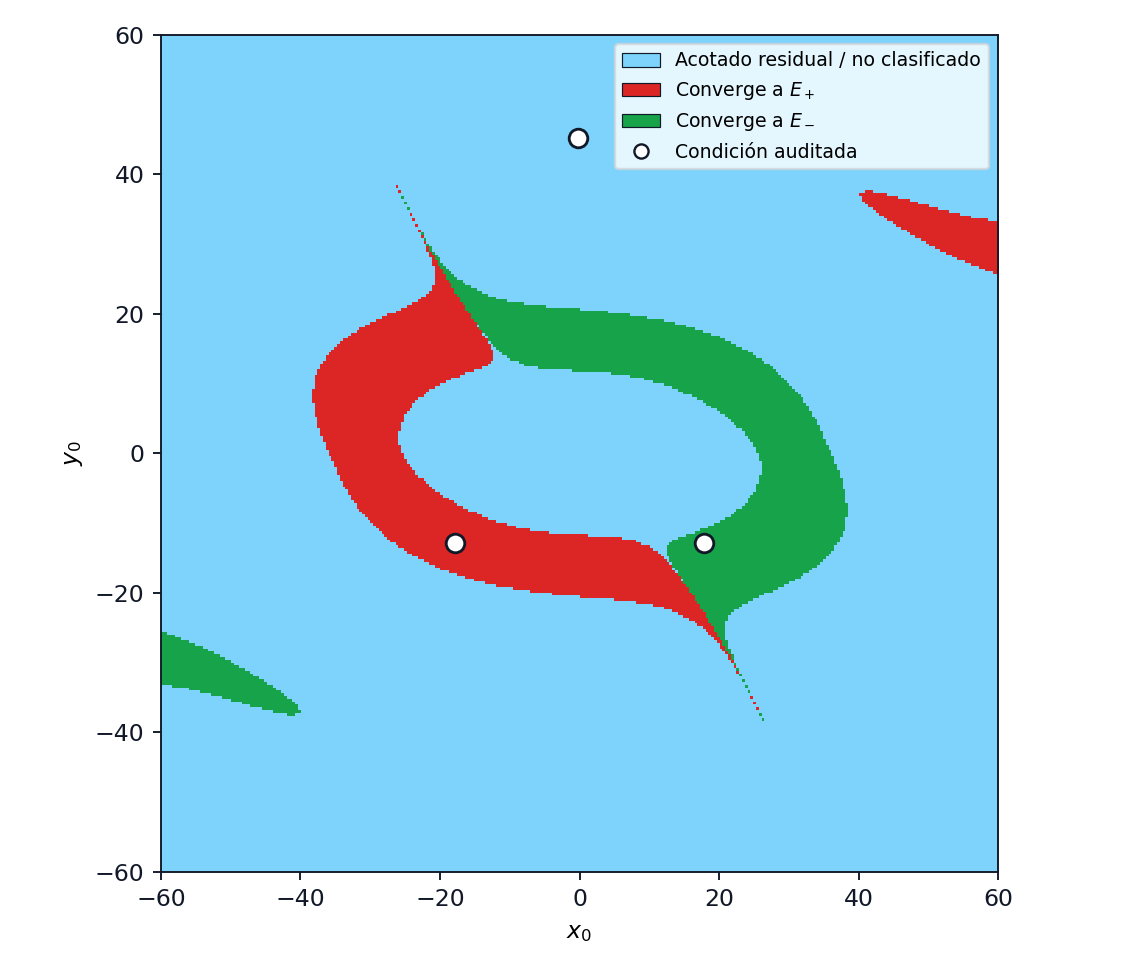
\includegraphics[width=0.84\linewidth]{lorenz_basin_reading_zones.png}
\caption{Zonas de lectura de una cuenca de Lorenz generada con Toolbox Chaos. Los
colores representan clases calculadas bajo un horizonte y un clasificador; las celdas
próximas a una frontera requieren refinamiento antes de asignarles etiquetas
asintóticas exactas.}
\label{fig:cuenca-profundizacion}
\end{figure}

\paragraph{Lectura de fronteras y dimensiones.}
Una pendiente sólo es defendible donde la gráfica log--log es aproximadamente lineal
y estable al añadir escalas. En una cuenca, las regiones interiores suelen ser más
robustas que la frontera. Conviene representar una clase separada para escapes,
indeterminación o no convergencia, en vez de forzar cada celda a un atractor.

\begin{warningbox}
Una dimensión estimada con dos escalas es sólo una pendiente. El antialiasing de una
imagen no contiene datos de cajas; deben usarse coordenadas o etiquetas exportadas.
La identificación de Wada requiere pruebas topológicas, y un valor de Kaplan--Yorke se complementa con una
estimación geométrica y evidencia de la medida invariante específica.
\end{warningbox}

\lecturaseccion{Kathleen T. Alligood, Tim D. Sauer y James A. Yorke,
\emph{Chaos: An Introduction to Dynamical Systems}, secciones 4.1, 4.4--4.7 y 5.3;
Robert L. Devaney, \emph{A First Course in Chaotic Dynamical Systems: Theory and
Experiment}, 2.\textsuperscript{a} ed., capítulo 14, apartados sobre fractales y
dimensión; Robert C. Hilborn, \emph{Chaos and Nonlinear Dynamics: An Introduction
for Scientists and Engineers}, 2.\textsuperscript{a} ed., capítulos 9--10, apartados
sobre dimensión fractal, correlación y multifractales; Tamás Tél y Márton Gruiz,
\emph{Chaotic Dynamics: An Introduction Based on Classical Mechanics}, capítulos
2 y 6.}

\subsection{Series temporales, FFT y densidad espectral}

\paragraph{Series temporales, FFT y PSD.}
Una serie uniformemente muestreada es \(s_n=s(n\Delta t)\), con frecuencia
\(f_s=1/\Delta t\). La transformada discreta
\[
 S_k=\sum_{n=0}^{N-1}s_n e^{-2\pi i kn/N}
\]
evalúa frecuencias \(f_k=kf_s/N\). Para una señal real, la parte unilateral contiene
frecuencias hasta Nyquist,
\[
 f_N=\frac{f_s}{2}.
\]
El \term{espectro de amplitud} describe magnitudes de componentes en un registro; la
\term{densidad espectral de potencia} distribuye potencia por frecuencia. Welch
promedia periodogramas de segmentos solapados y reduce varianza a cambio de resolución.

\paragraph{Ventanas, fuga y aliasing.}
Un registro finito equivale a multiplicar la señal por una ventana temporal. Si una
sinusoide no completa un número entero de periodos, su energía se reparte entre
frecuencias: \term{fuga espectral}. Una ventana suaviza discontinuidades en los
extremos, pero ensancha picos. Si existe contenido por encima de \(f_N\), el muestreo
lo refleja a frecuencias falsas: \term{aliasing}. Ninguna opción gráfica repara datos
ya submuestreados.

\paragraph{Ejemplo de frecuencias discretas.}
Con \(\Delta t=0.01\) y \(N=10000\),
\[
 f_s=100,\qquad f_N=50,\qquad
 \Delta f=\frac{f_s}{N}=0.01.
\]
Una señal \(s(t)=2\cos(2\pi\,1.5\,t)\) cae exactamente en el bin
\(k=1.5/0.01=150\) si el registro mantiene esa longitud. Si se reduce a
\(N=2000\), \(\Delta f=0.05\); el pico sigue localizable pero con malla cinco veces
más gruesa. Una señal de \(60\) Hz muestreada a \(100\) Hz aparece aliased cerca de
\(|60-100|=40\) Hz.

\begin{activitybox}{Práctica reproducible: una trayectoria, dos espectros}
Genere Lorenz clásico con RK4, \(dt=0.01\), \(T=200\), y descarte \(T_0=20\).
Pulse \gui{Usar última trayectoria} en \gui{Espectro}. Calcule primero
\gui{PSD de Welch (recomendado)} y después \gui{Espectro de amplitud}, sin cambiar
datos ni variable. Repita con \(T_0=50\) y con una trayectoria generada a
\(dt=0.005\). Exporte las series y compruebe \(f_s\), Nyquist, longitud útil y
resolución. Compare \(x\), \(y\) y \(z\) junto con el pico más alto.
\end{activitybox}

\begin{figure}[H]
\centering
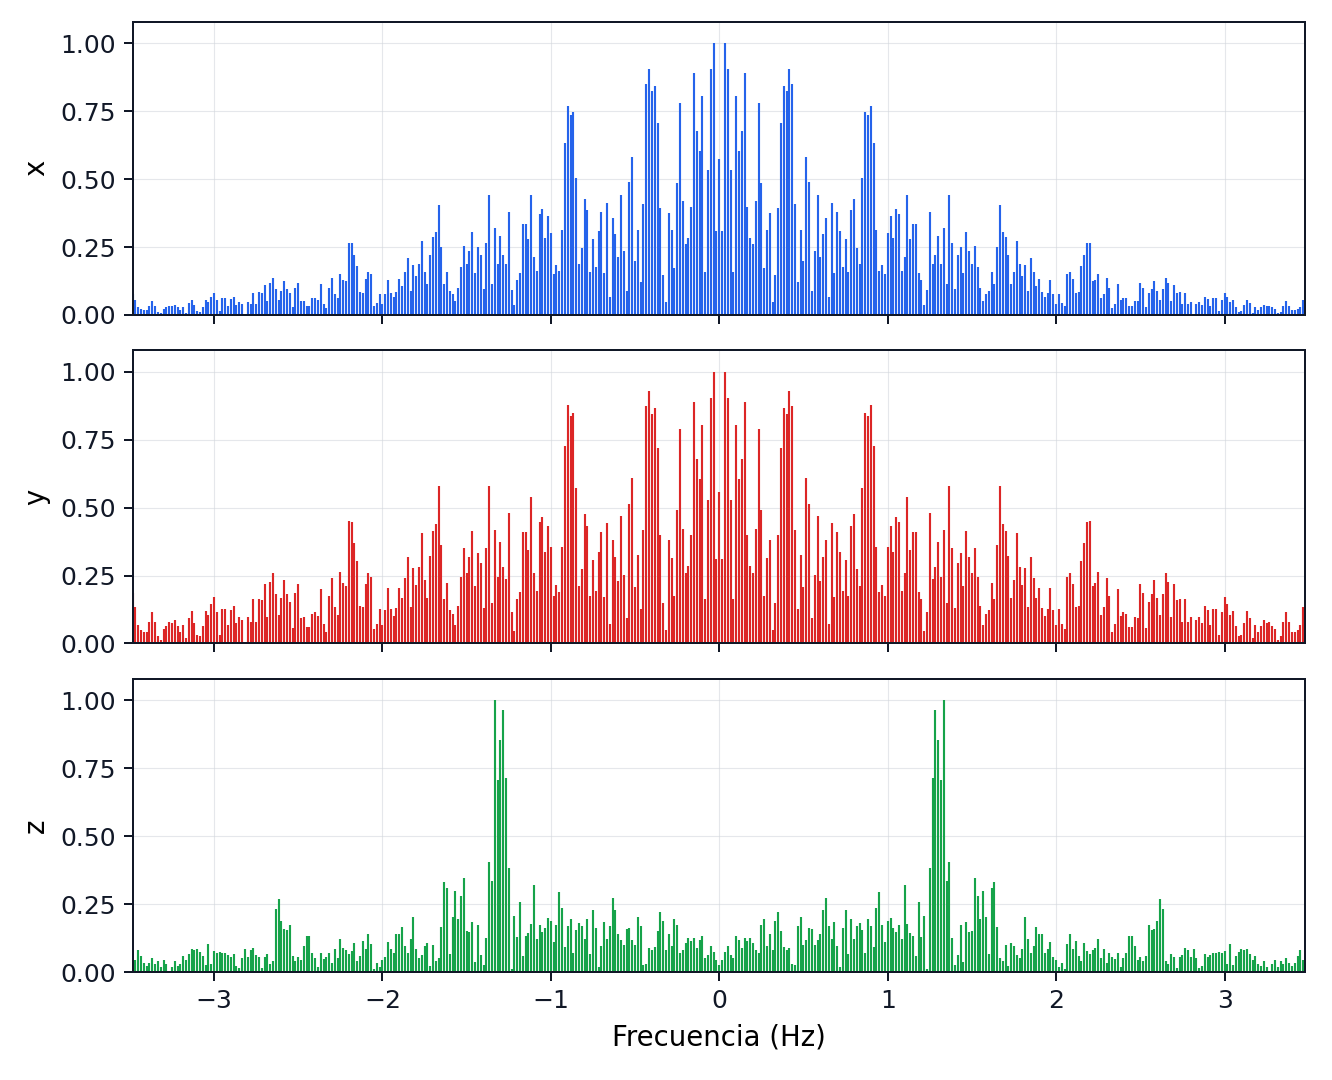
\includegraphics[width=0.80\linewidth]{lorenz_fft.png}
\caption{Espectro normalizado centrado de Lorenz generado a partir de datos del software. Los
picos y la banda describen el registro finito y su muestreo; su interpretación requiere
solos una prueba de caos.}
\label{fig:fft-profundizacion}
\end{figure}

\paragraph{Lectura de espectros y series.}
Una órbita periódica ideal produce líneas en la frecuencia fundamental y armónicos;
una cuasiperiódica, combinaciones de varias frecuencias inconmensurables; una señal
irregular puede mostrar banda ancha. Transitorios, ruido, modulación y no
estacionariedad también ensanchan el espectro. La serie original debe revisarse antes
de interpretar cada pico.

\begin{warningbox}
Un espectro ancho orienta el análisis de caos y un pico agudo orienta el de periodicidad
asintótica; ambos requieren pruebas dinámicas complementarias. Comparar amplitudes entre registros con distinta normalización, ventana o
duración es inválido. Welch mejora estabilidad estadística, pero no aumenta la
frecuencia de Nyquist ni recupera información perdida por aliasing.
\end{warningbox}

\lecturaseccion{Robert C. Hilborn, \emph{Chaos and Nonlinear Dynamics: An
Introduction for Scientists and Engineers}, 2.\textsuperscript{a} ed., apéndice A,
``Fourier Analysis'', y capítulo 9, apartados sobre cuantificación de series; Julien
C. Sprott, \emph{Elegant Chaos: Algebraically Simple Chaotic Flows}, capítulo 1,
apartados sobre espectros, ciclos, quasiperiodicidad e indicadores; Kathleen T.
Alligood, Tim D. Sauer y James A. Yorke, \emph{Chaos: An Introduction to Dynamical
Systems}, capítulo 13, apartado inicial sobre datos de series temporales.}

\subsection{Reconstrucción por retardo y diagnóstico desde una observación}

\paragraph{Vectores de reconstrucción por retardo.}
Cuando sólo se mide un escalar \(s(t)\), se forman vectores de retardo
\[
 \mathbf y_n=
 \bigl(s_n,s_{n-\ell},s_{n-2\ell},\ldots,s_{n-(m-1)\ell}\bigr),
\]
donde \(\tau=\ell\Delta t\) es el retardo y \(m\) la dimensión de inmersión. Bajo
hipótesis de suavidad, genericidad y dimensión suficiente, un teorema de inmersión
permite reconstruir una geometría equivalente en un sentido preciso. En datos
finitos, elegir \(\tau\), \(m\), observable y preprocesamiento es parte del resultado.

\paragraph{Selección de retardo y dimensión.}
Un retardo demasiado pequeño agrupa puntos cerca de la diagonal; uno demasiado grande
descorrelaciona las componentes y mezcla escalas. Se usan, como guías, el primer cruce
o mínimo de autocorrelación o información mutua. La dimensión puede explorarse con
falsos vecinos cercanos o saturación de una magnitud. Ningún umbral es universal.

\paragraph{Ejemplo algebraico resuelto: oscilador armónico.}
Sea \(s(t)=\cos(\omega t)\), con periodo \(T=2\pi/\omega\). Si
\(\tau=T/4\),
\[
 s(t-\tau)=\cos\left(\omega t-\frac{\pi}{2}\right)=\sin(\omega t),
\]
y por tanto
\[
 [s(t)]^2+[s(t-\tau)]^2=1.
\]
La reconstrucción bidimensional es un círculo. Si \(\tau=0\), todos los puntos caen
en la diagonal; si \(\tau=T/2\), caen en la antidiagonal. El mismo sistema puede
parecer degenerado por una elección inadecuada del retardo.

\begin{activitybox}{Práctica reproducible: reconstruir Lorenz desde \(x(t)\)}
En Toolbox Chaos genere Lorenz con \(dt=0.01\), \(T=200\) y descarte \(20\).
Exporte \(x(t)\). Calcule la autocorrelación y elija tres retardos: uno corto, el
primer cruce o escala equivalente, y uno cuatro veces mayor. Construya las nubes
\((x_n,x_{n-\ell})\) y
\((x_n,x_{n-\ell},x_{n-2\ell})\). Registre número de muestras efectivas después de
los desplazamientos. Repita con \(z(t)\) y explique qué rasgos dependen del observable.
\end{activitybox}

\paragraph{Lectura de reconstrucciones por retardo.}
Una reconstrucción útil separa estados sin convertir el conjunto en nube uniforme.
Las hebras cercanas pueden ser estructura o escasez de datos; deben revisarse con otro
retardo y más muestras. Un retrato de retorno \(s_{n+1}\) contra \(s_n\) aporta una representación distinta de
una inmersión general: sólo usa retraso de una muestra.

\begin{warningbox}
Una nube con forma de atractor no verifica las hipótesis de un teorema de inmersión.
La estimación de dimensión requiere puntos temporalmente separados, y el determinismo requiere más evidencia que una reconstrucción suave. Filtrar, normalizar o
interpolar cambia distancias y debe documentarse.
\end{warningbox}

\lecturaseccion{Kathleen T. Alligood, Tim D. Sauer y James A. Yorke,
\emph{Chaos: An Introduction to Dynamical Systems}, capítulo 13, apartados sobre
datos, coordenadas de retardo y embedología; Robert C. Hilborn,
\emph{Chaos and Nonlinear Dynamics: An Introduction for Scientists and Engineers},
2.\textsuperscript{a} ed., capítulo 10, apartados sobre inmersión, reconstrucción y
multifractales; Steven H. Strogatz, \emph{Nonlinear Dynamics and Chaos with
Applications to Physics, Biology, Chemistry, and Engineering},
2.\textsuperscript{a} ed., sección 12.4, ``Reconstructing Attractors from Data''.}

\subsection{Sistemas con retardo, alta dimensión e hipercaos}

\paragraph{Historia de estado en Mackey--Glass.}
En una ecuación con retardo,
\[
 \dot x(t)=F\bigl(x(t),x(t-\tau)\bigr),
\]
el valor \(x(0)\) se complementa con una función de historia que determina el futuro. Debe especificarse una función
historia \(\varphi(t)\) en \([-\tau,0]\). El espacio de estados es entonces
infinito-dimensional, aunque la salida se represente con unas pocas coordenadas de
retardo.

\paragraph{Ejemplo algebraico resuelto: Mackey--Glass.}
Una forma habitual es
\[
 \dot x(t)=
 \frac{\beta x(t-\tau)}{1+x^n(t-\tau)}-\gamma x(t).
\]
Un equilibrio constante \(x(t)=x^*\) satisface
\[
 0=x^*\left[\frac{\beta}{1+(x^*)^n}-\gamma\right].
\]
Además de \(x^*=0\), existe
\[
 x^*=\left(\frac{\beta}{\gamma}-1\right)^{1/n}
\]
si \(\beta>\gamma\). Para \(\beta=0.2\), \(\gamma=0.1\), \(n=10\),
\(x^*=1\). El equilibrio no depende de \(\tau\), pero su estabilidad sí: el retardo
entra en la ecuación característica trascendente de la linealización.

\paragraph{Alta dimensión: Lorenz--96.}
Con índices cíclicos,
\[
 \dot x_i=(x_{i+1}-x_{i-2})x_{i-1}-x_i+F,
 \qquad i=1,\ldots,N.
\]
El estado homogéneo \(x_i=F\) es equilibrio porque el término de advección se anula.
La divergencia es
\[
 \sum_{i=1}^{N}\frac{\partial\dot x_i}{\partial x_i}=-N,
\]
de modo que el modelo contrae volumen en el espacio \(N\)-dimensional. Alta dimensión
requiere criterios adicionales para \term{hipercaos}; esta etiqueta suele requerir más de un exponente de
Lyapunov positivo convergente.

\begin{activitybox}{Práctica reproducible: historia y proyección}
Ejecute el preset de Mackey--Glass y registre \(\beta,\gamma,n,\tau\), historia,
paso y esquema numérico mostrado por la interfaz. Duplique el horizonte y compare
series y retratos de retardo. Después ejecute Lorenz--96 con la dimensión y forzamiento
del preset; grafique tres componentes contiguas y tres separadas. Exporte las series y
compare correlaciones y escalas. Si \gui{Lyapunov} aparece como no disponible,
consérvelo como límite del contrato y no transfiera el algoritmo 3D.
\end{activitybox}

\begin{figure}[H]
\centering
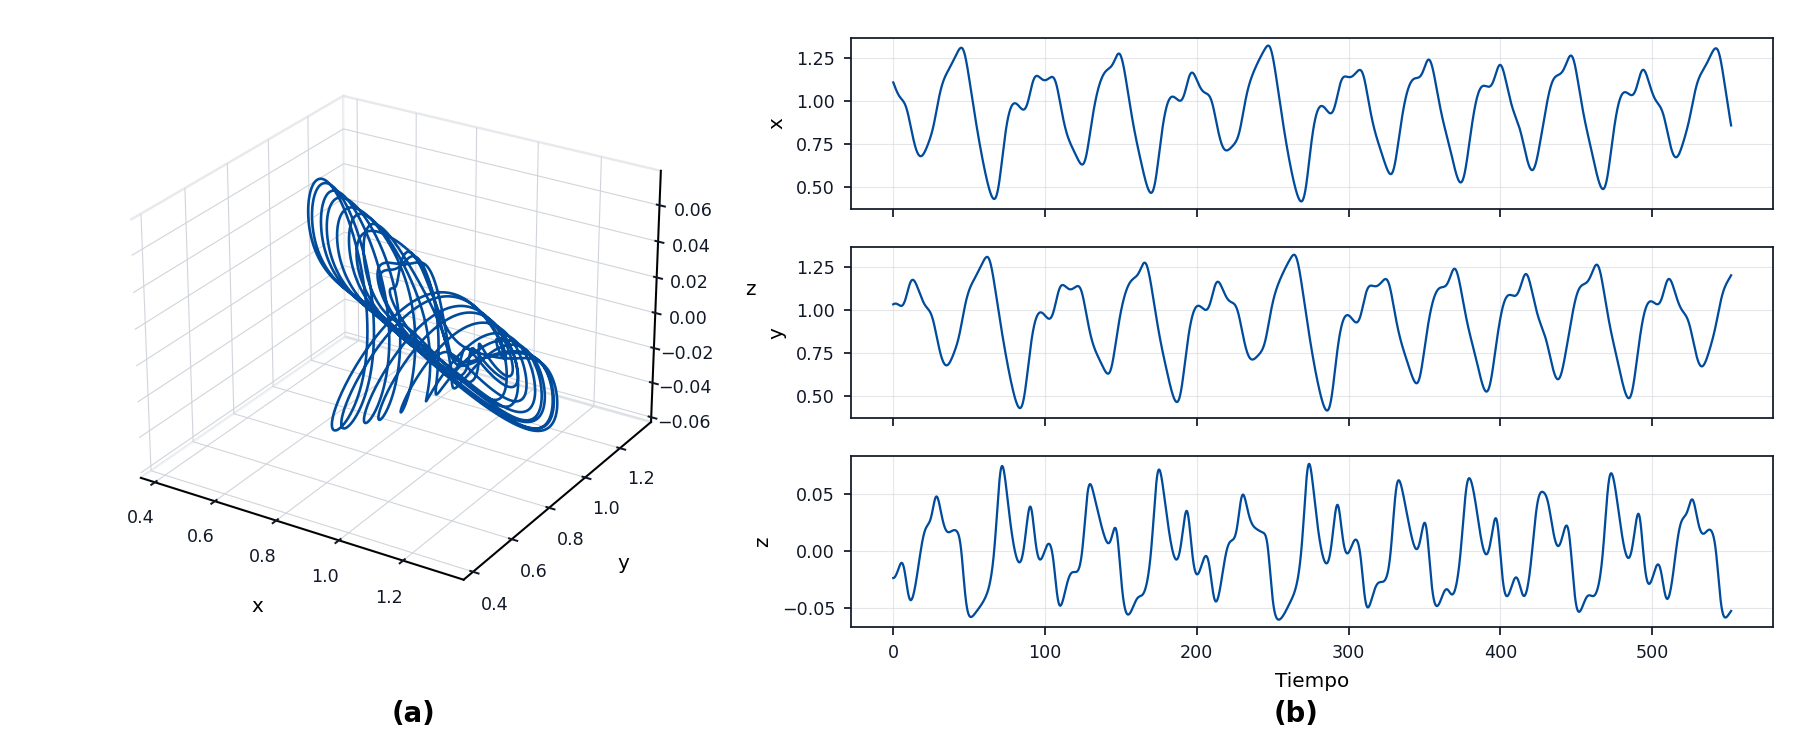
\includegraphics[width=0.88\linewidth]{systems/mackey_glass_phase_timeseries.png}
\caption{Mackey--Glass generado por Toolbox Chaos. La proyección usa retardos o
componentes derivadas de una historia; conserva la naturaleza funcional de la ecuación y requiere el marco adecuado de EDO
tridimensional.}
\label{fig:mackey-glass-profundizacion}
\end{figure}

\begin{figure}[H]
\centering
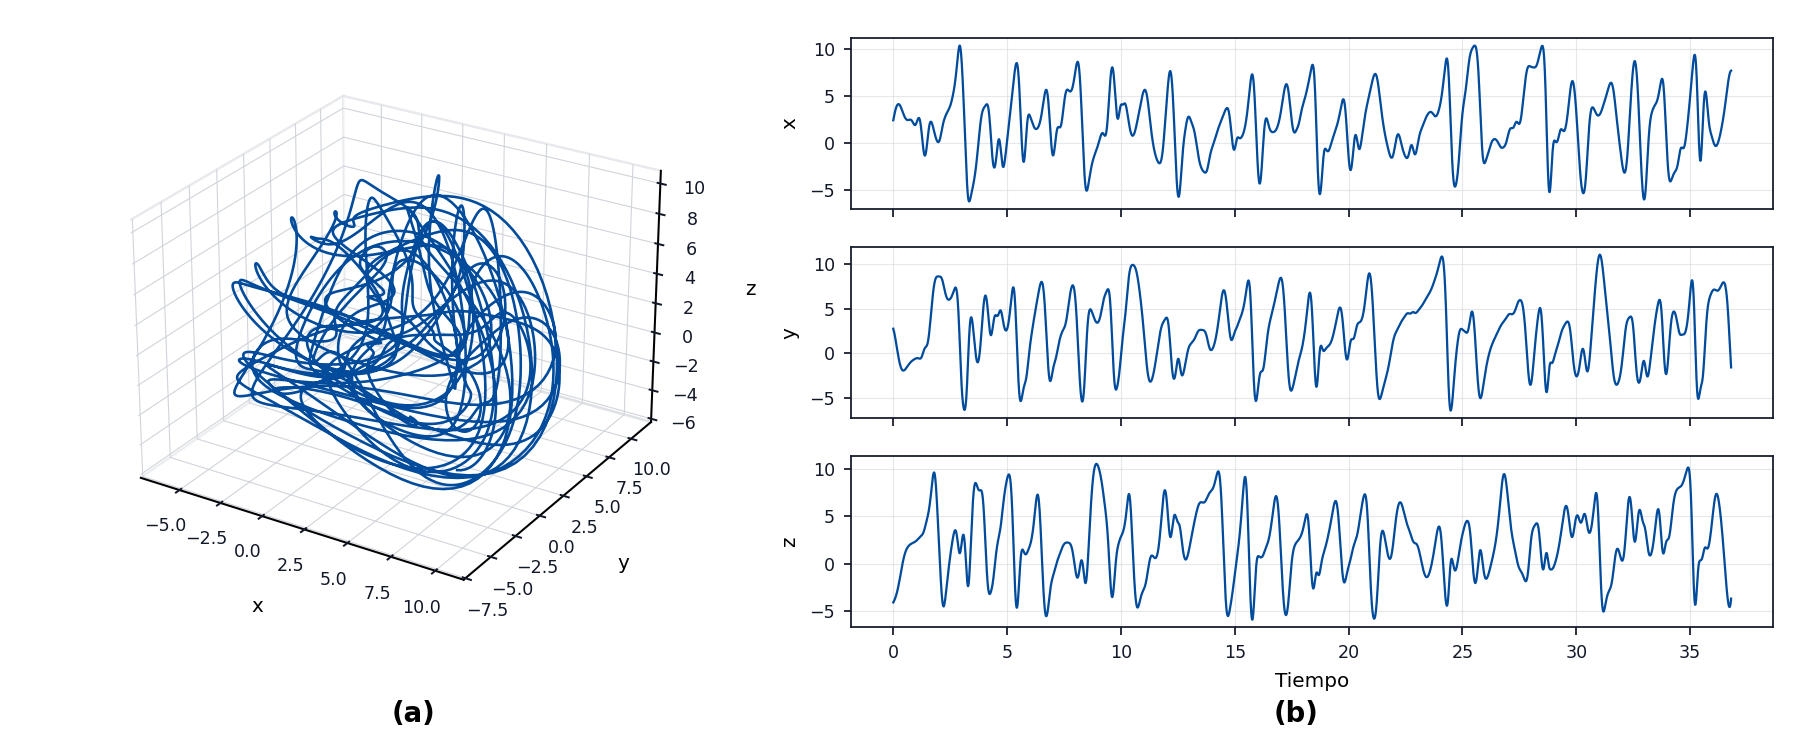
\includegraphics[width=0.88\linewidth]{systems/lorenz96_phase_timeseries.png}
\caption{Lorenz--96 generado por Toolbox Chaos. Tres coordenadas muestran una sombra
del estado de dimensión mayor; la estructura omitida debe discutirse antes de inferir
geometría global.}
\label{fig:lorenz96-profundizacion}
\end{figure}

\paragraph{Lectura de sistemas con retardo y alta dimensión.}
En retardo, una transición depende de la historia junto con el valor final.
En alta dimensión, dos proyecciones distintas pueden ocultar o crear cruces aparentes.
La presencia de varias escalas temporales sugiere calcular correlaciones, espectros y,
cuando exista un método compatible, varios exponentes.

\begin{warningbox}
Use una historia completa para representar el estado. Clasifique como hipercaótico
un sistema por tener cuatro o más variables, ni extrapole un espectro de Lyapunov 3D
a dimensión alta. Una señal irregular de Mackey--Glass o Lorenz--96 puede incluir un
transitorio largo y requiere prueba de horizonte.
\end{warningbox}

\lecturaseccion{Julien C. Sprott, \emph{Elegant Chaos: Algebraically Simple Chaotic
Flows}, capítulo 6, apartados sobre sistemas de alta dimensión e hipercaos, capítulo
8, ``Spatiotemporal Chaos'', y capítulo 9, ``Delay Differential Equations''; Robert
C. Hilborn, \emph{Chaos and Nonlinear Dynamics: An Introduction for Scientists and
Engineers}, 2.\textsuperscript{a} ed., capítulo 11, apartados sobre caos
espaciotemporal; Tamás Tél y Márton Gruiz, \emph{Chaotic Dynamics: An Introduction
Based on Classical Mechanics}, capítulo 3, apartados sobre estabilidad y espacio de
fases general.}

\subsection{Caos conservativo y caos transitorio}

\paragraph{Estructura de los sistemas conservativos.}
En un sistema hamiltoniano
\[
 \dot q=\frac{\partial H}{\partial p},\qquad
 \dot p=-\frac{\partial H}{\partial q},
\]
se cumple \(\dot H=0\) y la divergencia del campo es cero. No hay atracción
volumétrica como en Lorenz. El espacio de fases puede mezclar islas regulares, toros y
mares caóticos; hablar de atractor en el sentido disipativo suele ser inapropiado.

\paragraph{Ejemplo algebraico resuelto: mapa estándar.}
El mapa
\[
 p_{n+1}=p_n+K\sin q_n,\qquad
 q_{n+1}=q_n+p_{n+1}\pmod{2\pi}
\]
tiene Jacobiano
\[
 D F=
 \begin{pmatrix}
 1+K\cos q_n&1\\
 K\cos q_n&1
 \end{pmatrix},
\qquad \det DF=1.
\]
Por tanto preserva área exactamente en aritmética matemática. Para \(K=0\),
\(p_n=p_0\) y \(q_n=q_0+np_0\); el número de rotación es \(p_0/(2\pi)\). Al aumentar
\(K\), resonancias y capas caóticas pueden coexistir sin contracción global.

\paragraph{Tiempo de escape y caos transitorio.}
Una silla caótica no atractora puede retener órbitas durante tiempos irregulares antes
de que escapen. Si la probabilidad de supervivencia se aproxima por
\[
 P(t)\simeq e^{-\kappa t},
\]
\(\kappa\) es una tasa de escape y el tiempo medio idealizado es \(1/\kappa\). Si de
1000 semillas quedan cerca de 368 a \(t=10\), entonces
\[
 \widehat\kappa=-\frac1{10}\log(368/1000)\simeq0.10,
\qquad \widehat{\langle T\rangle}\simeq10.
\]
La estimación de esta distribución requiere un conjunto de trayectorias y condiciones iniciales.

\begin{activitybox}{Práctica reproducible: conservación y supervivencia}
En \gui{Crear sistema}, defina el oscilador
\(\dot q=p,\ \dot p=-q\) con \((q_0,p_0)=(1,0)\). Para Euler, Heun y RK4 y
\(h=0.05,0.025,0.0125\), exporte \(H_n=(q_n^2+p_n^2)/2\) y grafique su deriva.
Después seleccione un caso del catálogo que muestre escape o transitorio prolongado,
si está disponible, y ejecute una malla explícita de condiciones iniciales con dos
horizontes. Construya una curva de supervivencia sin reclasificar escapes como
atractores.
\end{activitybox}

\paragraph{Lectura de trayectorias conservativas y transitorias.}
En dinámica conservativa, puntos que llenan una curva indican movimiento regular
confinado; nubes e islas pueden coexistir. La deriva sistemática de energía revela
efecto del integrador, no disipación física. En caos transitorio, se debe graficar
número de sobrevivientes en escala semilogarítmica y comprobar si existe un intervalo
aproximadamente lineal.

\begin{warningbox}
En un sistema conservativo, una trayectoria acotada debe analizarse mediante invariantes y estructura de volumen antes de clasificarla como atractor. Un determinante
numérico cercano a uno se complementa con controles de conservación. El horizonte finito
censura tiempos de escape, por lo que las irregularidades requieren extender la simulación y comparar condiciones iniciales.
\end{warningbox}

\lecturaseccion{Robert C. Hilborn, \emph{Chaos and Nonlinear Dynamics: An
Introduction for Scientists and Engineers}, 2.\textsuperscript{a} ed., capítulo 4,
apartados sobre transitorios caóticos y órbitas homoclínicas, y capítulo 8, apartados
sobre dinámica hamiltoniana, KAM, mapa estándar y Hénon--Heiles; Tamás Tél y Márton
Gruiz, \emph{Chaotic Dynamics: An Introduction Based on Classical Mechanics},
capítulo 6, ``Transient Chaos'', y capítulo 7, apartados sobre dinámica conservativa,
mapa estándar, ergodicidad y mezcla; Julien C. Sprott, \emph{Elegant Chaos:
Algebraically Simple Chaotic Flows}, capítulo 4, apartados sobre flujos conservativos.}

\subsection{Sincronización y control de caos}

\paragraph{Sincronización y variables de error.}
Dos sistemas se \term{sincronizan} cuando una medida de su diferencia converge o
permanece pequeña bajo un acoplamiento especificado. La sincronía completa usa
\(\|\mathbf x_1-\mathbf x_2\|\to0\); existen también sincronía de fase, generalizada
y retrasada. \term{Control de caos} introduce una intervención pequeña y diseñada
para estabilizar una órbita o región deseada. La evaluación del control declara señal, ley de control, costo y estabilidad del lazo cerrado.

\paragraph{Dinámica transversal del error.}
Para dos sistemas idénticos con acoplamiento difusivo completo,
\[
 \dot{\mathbf x}_1=\mathbf f(\mathbf x_1),\qquad
 \dot{\mathbf x}_2=\mathbf f(\mathbf x_2)+k(\mathbf x_1-\mathbf x_2),
\]
el error \(\mathbf e=\mathbf x_2-\mathbf x_1\) satisface, cerca de la variedad
sincrónica,
\[
 \dot{\mathbf e}\simeq
 [D\mathbf f(\mathbf x_1(t))-kI]\mathbf e.
\]
La estabilidad depende de la expansión transversal a lo largo de la trayectoria, no
sólo de los autovalores en un equilibrio.

\paragraph{Ejemplo algebraico resuelto.}
Para el par lineal
\[
 \dot x=-ax,\qquad \dot y=-ay+k(x-y),
\]
\(e=y-x\) cumple
\[
 \dot e=-(a+k)e,\qquad e(t)=e(0)e^{-(a+k)t}.
\]
Si \(a=0.2\), \(k=0.8\), el error disminuye con tasa \(1\). Sin acoplamiento,
\(k=0\), disminuye con tasa \(0.2\). Este ejemplo separa sincronización inducida de
la convergencia común a un equilibrio; en un sistema caótico, cada trayectoria puede
seguir siendo irregular mientras el error transversal decrece.

\paragraph{Control en un mapa linealizado.}
Si cerca de una órbita objetivo el mapa controlado es
\[
 \xi_{n+1}=a\xi_n+b u_n,\qquad u_n=-K\xi_n,
\]
el multiplicador cerrado es \(a-bK\). Para \(a=1.2\), \(b=1\), elegir \(K=0.5\)
produce \(0.7\), estable. Debe comprobarse que la linealización y los límites del
actuador sean válidos en la región usada.

\begin{activitybox}{Práctica reproducible: error de dos Lorenz}
En \gui{Crear sistema}, defina dos copias de Lorenz con variables
\texttt{x1,y1,z1,x2,y2,z2}. La primera usa las ecuaciones clásicas; en la segunda
añada \texttt{k*(x1-x2)}, \texttt{k*(y1-y2)} y \texttt{k*(z1-z2)} a las tres
ecuaciones. Use \((10,28,8/3)\), estados \((1,1,1)\) y \((1.001,1,1)\),
\(k=0,1,5\), RK4, \(h=0.005\), \(T=50\). Exporte datos y grafique
\(\log\|\mathbf e(t)\|\), evitando el logaritmo de cero. Repita con \(h/2\) y
registre la magnitud del acoplamiento.
\end{activitybox}

\paragraph{Lectura del error de sincronización.}
La sincronización se evalúa en el error, no por superposición visual de dos curvas
gruesas. Una recta descendente en escala semilogarítmica sugiere contracción
exponencial transversal en ese intervalo. En control, compare régimen sin control,
transitorio de activación, estado controlado y esfuerzo \(u(t)\).

\begin{warningbox}
La estabilidad global de la variedad sincrónica requiere controles más amplios que un
error pequeño durante tiempo finito. Las pruebas de robustez usan perturbaciones de las condiciones iniciales. Un controlador que satura, cambia mucho el modelo o
requiere conocer toda la trayectoria debe reportarse con esas condiciones de uso;
estabilización de pequeña señal.
\end{warningbox}

\lecturaseccion{Robert C. Hilborn, \emph{Chaos and Nonlinear Dynamics: An
Introduction for Scientists and Engineers}, 2.\textsuperscript{a} ed., capítulo 12,
apartados sobre control y sincronización; Julien C. Sprott,
\emph{Elegant Chaos: Algebraically Simple Chaotic Flows}, capítulo 1, apartados sobre
exponentes, estabilidad y transitorios, y capítulo 10, apartados sobre realizaciones
en circuitos; John Guckenheimer y Philip Holmes, \emph{Nonlinear Oscillations,
Dynamical Systems, and Bifurcations of Vector Fields}, capítulo 4, apartados sobre
perturbaciones y métodos de Melnikov, como contexto de intervención débil.}

\section{Proyecto final sobre un sistema dinámico}

\paragraph{Pregunta y evidencia del proyecto.}
El proyecto integra un resultado analítico con evidencia numérica. La pregunta debe
ser acotada, por ejemplo: ¿cómo cambia un régimen al variar un parámetro?, ¿qué
condiciones iniciales alcanzan dos destinos?, ¿qué propiedad permanece al refinar el
paso?, ¿qué observable distingue periodicidad de irregularidad? El informe acepta como
pregunta únicamente ``graficar un atractor''.

\paragraph{Opciones de proyecto.}
\begin{enumerate}
  \item \textbf{Mapa:} logística, Hénon o sistema del \gui{Explorador Sprott};
  incluir puntos periódicos, multiplicadores, bifurcación y dinámica simbólica.
  \item \textbf{Flujo clásico:} Lorenz, Rössler, Chua o Duffing--Ueda; incluir
  equilibrios, Jacobiano, disipación, sección y al menos un indicador.
  \item \textbf{Cuencas y coexistencia:} comparar condiciones iniciales, resolución,
  horizonte y clasificador, con categoría indeterminada.
  \item \textbf{Datos:} reconstruir una dinámica desde una serie, justificar muestreo,
  FFT/PSD, retardo, dimensión y control sustituto.
  \item \textbf{Extensión:} retardo, alta dimensión, caos transitorio,
  sincronización o memoria fraccionaria, con alcance explícitamente prudente.
\end{enumerate}

\paragraph{Desarrollo algebraico obligatorio.}
El informe debe incluir al menos uno de los siguientes cálculos completos:
\begin{itemize}
  \item puntos fijos o equilibrios y clasificación mediante derivada o Jacobiano;
  \item adimensionalización y grupos de control;
  \item multiplicador de órbita o forma normal local;
  \item divergencia, invariante o balance de energía;
  \item ecuación variacional y significado del indicador de Lyapunov;
  \item solución de equilibrio para un sistema con retardo;
  \item dinámica del error para sincronización o control.
\end{itemize}
Copiar ecuaciones del catálogo sin desarrollar una consecuencia no satisface este
requisito.

\paragraph{Protocolo computacional mínimo.}
\begin{enumerate}
  \item Registrar nombre del sistema, ecuaciones, parámetros y unidades o escalas.
  \item Guardar condición o historia inicial, método, paso, tolerancias, horizonte,
  transitorio, muestreo y umbral de escape.
  \item Producir tres vistas coordinadas desde los mismos datos cuando sea posible.
  \item Exportar datos y metadatos junto con las imágenes.
  \item Repetir con al menos dos pasos u opciones de tolerancia.
  \item Repetir con horizonte o transitorio distinto.
  \item Comparar condiciones iniciales si la pregunta es global.
  \item Explicar disponibilidad y limitación de cada pestaña utilizada.
\end{enumerate}

\begin{evidencebox}{Matriz de afirmaciones del proyecto}
Para cada conclusión, incluya cuatro columnas: afirmación; evidencia directa;
control de robustez; y alternativa no descartada. Ejemplo: ``la estimación finita de
\(\lambda_1\) es positiva'' se apoya en la curva de convergencia y dos refinamientos;
describe el conjunto de estados y parámetros que cubre la evidencia declarada.
\end{evidencebox}

\paragraph{Estructura del informe.}
\begin{longtable}{>{\raggedright\arraybackslash}p{0.23\linewidth}
                  >{\raggedright\arraybackslash}p{0.67\linewidth}}
\toprule
Sección & Contenido verificable \\
\midrule
\endhead
Pregunta y alcance & Variable de respuesta, parámetro o comparación y límites.\\
Modelo & Ecuaciones, estado, hipótesis, unidades y procedencia del preset.\\
Análisis & Desarrollo algebraico y predicción anterior a la simulación.\\
Método & Contrato numérico completo y versión del software.\\
Resultados & Datos, tablas, tres vistas, pies autosuficientes e indicador.\\
Robustez & Paso, horizonte, transitorio, semilla y, cuando proceda, resolución.\\
Discusión & Coincidencias y tensiones entre predicción, gráfica e indicador.\\
Conclusión & Respuesta graduada y lista de propiedades no demostradas.\\
Anexo & Archivos JSON/CSV, nombres de figuras y guía de reproducción.\\
\bottomrule
\end{longtable}

\begin{activitybox}{Reproducción cruzada}
Entregue a otro equipo una carpeta que contenga únicamente informe, configuración y
datos. El equipo receptor repite una figura y un valor cuantitativo sin explicación
oral. Debe registrar versión, diferencias y ambigüedades. El equipo autor corrige el
protocolo y conserva ambas ejecuciones como evidencia de trazabilidad.
\end{activitybox}

\begin{warningbox}
El proyecto formula conclusiones acordes con muestreos finitos. Las expresiones ``demuestra caos'', ``prueba estabilidad global'' o ``valida el
modelo físico'' requieren un argumento matemático específico con todas sus hipótesis y evidencia adicional a una pestaña o una figura.
\end{warningbox}

\lecturaseccion{Edward N. Lorenz, \emph{The Essence of Chaos}, capítulos 1--5 y
apéndices ``The Butterfly Effect'', ``Mathematical Excursions'' y ``Glossary'', como
modelo de conexión entre mecanismo, cálculo e interpretación; Robert C. Hilborn,
\emph{Chaos and Nonlinear Dynamics: An Introduction for Scientists and Engineers},
2.\textsuperscript{a} ed., capítulos 9--10, sobre cuantificación y reconstrucción;
Kathleen T. Alligood, Tim D. Sauer y James A. Yorke,
\emph{Chaos: An Introduction to Dynamical Systems}, apéndice B, para control de error
numérico.}

\section[\texorpdfstring{\hspace{0.45em}}{}Banco graduado de actividades y problemas]{Banco graduado de actividades y problemas}

\paragraph{Estructura de actividades A--C.}
Las actividades A son de interpretación, las B combinan álgebra y simulación, y las C
constituyen miniproyectos. En todos los casos se entrega predicción previa, contrato
numérico, figura con ejes, datos exportados, control y evidencia pendiente por documentar.

\subsection*{Nivel A: lectura y conceptos}
\begin{enumerate}
  \item[A1.] \textbf{Misma órbita, tres vistas.} Use Lorenz y marque en
  \gui{Atractor 3D}, \gui{Retratos 2D} y \gui{Series temporales} el mismo intervalo.
  Explique qué información pierde cada vista.
  \item[A2.] \textbf{Mapa y flujo: reglas de actualización.} Para veinte puntos logísticos, compare una
  gráfica con marcadores y otra con líneas. Identifique qué segmentos no pertenecen a
  la dinámica.
  \item[A3.] \textbf{Nullcline y trayectoria: funciones complementarias.} Sobre el ejemplo
  \(\dot x=x(1-x-y)\), \(\dot y=y(x-1/2)\), señale dónde el vector es vertical y
  dónde horizontal.
  \item[A4.] \textbf{Transitorio.} Para Rössler, grafique las primeras y las últimas
  veinte unidades de tiempo con la misma escala. Decida qué estadísticas cambian.
  \item[A5.] \textbf{Proyección engañosa.} Localice un cruce en \(x\)-\(y\) de
  Lorenz y compare las coordenadas \(z\) y los tiempos de ambos puntos.
  \item[A6.] \textbf{Pie de figura auditable.} Reescriba el pie de una captura para
  incluir sistema, parámetros, estado, método, paso, tiempo, transitorio y mensaje
  principal.
\end{enumerate}

\subsection*{Nivel B: cálculo y reproducción}
\begin{enumerate}
  \item[B1.] \textbf{Saddle--node.} Derive ramas y estabilidad de
  \(\dot x=\mu-x^2\); mida el tiempo para entrar en una tolerancia de \(10^{-3}\)
  cuando \(\mu\) se aproxima a cero.
  \item[B2.] \textbf{Plano traza--determinante.} Diseñe una matriz para cada región,
  calcule sus autovalores y reproduzca los retratos en \gui{Crear sistema}.
  \item[B3.] \textbf{Jacobiano de Lorenz.} Derive \(J(x,y,z)\), evalúelo en
  \(E_0,E_\pm\) y confronte \gui{Autovalores} para dos valores de \(\rho\).
  \item[B4.] \textbf{Ciclo radial.} Estime periodo y multiplicador del ciclo
  \(r=1\) con dos pasos; compare con \(2\pi\) y \(e^{-4\pi}\).
  \item[B5.] \textbf{Periodo dos logístico.} Para \(r=3.2\), verifique
  \(x_\pm\), su orden temporal y el multiplicador \(M_2=0.16\).
  \item[B6.] \textbf{Contracción de Hénon.} Seleccione tres triángulos pequeños de
  condiciones iniciales, itere una vez y compare áreas con el factor \(|b|\).
  \item[B7.] \textbf{Divergencia.} Calcule \(\nabla\cdot f\) para Lorenz, Rössler y
  Duffing autónomo; relacione signo instantáneo con el volumen, sin inferir cuenca.
  \item[B8.] \textbf{Convergencia Lyapunov.} Para Lorenz, combine dos pasos, dos
  tiempos finales y dos intervalos QR. Informe sólo dígitos estables.
  \item[B9.] \textbf{Nyquist.} Genere dos señales sintéticas en
  \gui{Crear sistema} o desde datos controlados, una debajo y otra encima de Nyquist;
  identifique el alias en \gui{Espectro}.
  \item[B10.] \textbf{Reconstrucción.} Para una señal periódica, compruebe que
  \(\tau=T/4\) produce un círculo y que \(\tau=0\) produce una diagonal.
  \item[B11.] \textbf{Dimensión de cajas.} Valide el algoritmo con etapas del Cantor
  antes de aplicarlo a una frontera de cuenca.
  \item[B12.] \textbf{Energía numérica.} Compare deriva de \(H\) para Euler, Heun y
  RK4; interprete la menor deriva como un indicador que se complementa con la prueba de conservación.
\end{enumerate}

\subsection*{Nivel C: miniproyectos}
\begin{enumerate}
  \item[C1.] \textbf{Ventana periódica.} Localice una ventana logística, verifique
  periodo, multiplicador y \(\lambda_N\), y estudie sus bordes.
  \item[C2.] \textbf{Retorno de Rössler.} Defina una sección, interpole cruces,
  construya \(u_{n+1}\) contra \(u_n\) y discuta si es aproximadamente unimodal.
  \item[C3.] \textbf{Ruta de Duffing.} Varíe un solo parámetro, compare secciones
  estroboscópicas y clasifique la evidencia de periodicidad, toro o irregularidad.
  \item[C4.] \textbf{Frontera de cuenca.} Refine resolución y horizonte, estime una
  pendiente y cuantifique celdas que cambian de clase.
  \item[C5.] \textbf{Mackey--Glass.} Compare dos historias con el mismo \(x(0)\);
  muestre cómo la historia completa define el estado.
  \item[C6.] \textbf{Lorenz--96.} Compare proyecciones contiguas y separadas, PSD y
  correlaciones; explique qué queda fuera de la vista.
  \item[C7.] \textbf{Caos transitorio.} Construya una distribución de tiempos de
  escape con datos censurados y pruebe un ajuste exponencial sólo en el intervalo
  sustentado.
  \item[C8.] \textbf{Sincronización.} Estime una tasa transversal desde
  \(\log\|\mathbf e(t)\|\), explore \(k\) y cuantifique el costo de acoplamiento.
  \item[C9.] \textbf{Acceso a coexistencia.} Compare semillas cercanas a equilibrios
  y alejadas; clasifique la evidencia sin convertir ausencia finita en ocultamiento.
  \item[C10.] \textbf{Explorador Sprott.} Elija un código sintético público,
  decodifique sus coeficientes, derive sus ecuaciones, calcule puntos fijos cuando
  proceda y conserve código, datos, estilo y metadatos.
\end{enumerate}

\begin{evidencebox}{Criterio de cierre del banco}
Una actividad está terminada cuando otra persona puede repetirla, la predicción
algebraica se contrasta con los datos, el rasgo interpretado sobrevive al control
elegido y la conclusión se mantiene dentro del alcance del método. Obtener una imagen aporta
criterio de cierre.
\end{evidencebox}

\begin{warningbox}
Las actividades que requieren cálculos externos parten de datos exportados por
Toolbox Chaos y deben conservar el script o procedimiento usado. Las atribuciones deben corresponder
a la interfaz estimadores que no implementa, ni ocultar pasos manuales bajo frases
como ``el software demostró''. Cada herramienta se acredita por la operación que
realmente realizó.
\end{warningbox}

\lecturaseccion{Para seleccionar problemas adicionales: Robert L. Devaney,
\emph{A First Course in Chaotic Dynamical Systems: Theory and Experiment},
2.\textsuperscript{a} ed., capítulos 3--14; Kathleen T. Alligood, Tim D. Sauer y
James A. Yorke, \emph{Chaos: An Introduction to Dynamical Systems}, capítulos 1--13
y apéndice B; Julien C. Sprott, \emph{Elegant Chaos: Algebraically Simple Chaotic
Flows}, capítulos 1--10; Julien C. Sprott, \emph{Strange Attractors: Creating
Patterns in Chaos}, secciones 2.3--2.4, 3.1--3.5, capítulos 4--6 y apéndices E--F.}


\section[\texorpdfstring{\hspace{0.45em}}{}Interpretación y comunicación de resultados]{Interpretación y comunicación de resultados}
\lecturaseccion{Edward N. Lorenz, \emph{The Essence of Chaos}, capítulos 1--5; Robert C. Hilborn, \emph{Chaos and Nonlinear Dynamics}, capítulos 9--10; Julien C. Sprott, \emph{Elegant Chaos}, secciones 1.1--1.15.}

La interpretación final requiere una secuencia que conecte gráficas, indicadores y
controles numéricos, de modo que las conclusiones sean auditables y proporcionales a la
evidencia. Las pestañas forman una secuencia de resultados conectados. Cada una responde una
pregunta y prepara la siguiente. Una buena investigación avanza desde la verificación
básica de la trayectoria hasta diagnósticos globales y pruebas de robustez.

Un ``resultado reproducible'' puede representarse como la tupla
\[
 \mathcal E=(f,\boldsymbol\mu,\mathbf{x}_0,\mathcal M,h,T,T_0,
 \mathcal O,\mathcal C),
\]
donde $f$ es el modelo, $\mathcal M$ el método, $\mathcal O$ la observable y
$\mathcal C$ los criterios de clasificación. La figura es una función de
$\mathcal E$, dentro de un protocolo reproducible.

Con esa tupla como referencia, la siguiente ruta conserva una pregunta por etapa:
\begin{enumerate}
  \item \gui{Series temporales}: ¿escapa, converge o mantiene un régimen acotado?
  \item \gui{Comparar metodos}: ¿la característica sobrevive al refinamiento?
  \item \gui{Atractor 3D} y \gui{Retratos 2D}: ¿qué geometría y simetrías aparecen?
  \item \gui{Autovalores}: ¿qué predice la dinámica local de los equilibrios?
  \item \gui{Bifurcación}: ¿cómo cambia el régimen con el parámetro?
  \item \gui{Cuenca de atracción} y \gui{Coexistencia}: ¿qué destinos dependen de la condición inicial?
  \item \gui{Lyapunov}: ¿existe expansión media convergente?
  \item \gui{Espectro}: ¿qué escalas temporales dominan y son consistentes con las series?
\end{enumerate}

Al terminar el recorrido, una redacción proporcionada sería: ``Para los parámetros
indicados, las trayectorias
permanecieron acotadas durante $T$; el exponente máximo finito fue positivo y mostró
una meseta estable al duplicar el horizonte; el diagrama de bifurcación presentó una
nube persistente después de duplicar el transitorio. Estos resultados son consistentes
con dinámica caótica en el régimen numérico estudiado.'' La formulación mantiene el
alcance del cálculo y reserva las propiedades adicionales para la evidencia correspondiente.

\begin{longtable}{>{\raggedright\arraybackslash}p{0.16\textwidth}
                  >{\raggedright\arraybackslash}p{0.24\textwidth}
                  >{\raggedright\arraybackslash}p{0.25\textwidth}
                  >{\raggedright\arraybackslash}p{0.25\textwidth}}
\toprule
Gráfica o cálculo & Pregunta principal & Señal útil & Control antes de concluir\\
\midrule
\endhead
Atractor 3D & ¿Qué región visita la órbita? & Geometría, simetría, acotación visible & Más condiciones iniciales, más tiempo y otras proyecciones\\
Series temporales & ¿Cómo evoluciona cada variable? & Tendencia, oscilación, transitorio & Paso, horizonte, saturación y escala de ejes\\
Retratos 2D & ¿Cómo se relacionan pares de variables? & Lazos, pliegues, proyecciones & Verificar cruces aparentes en dimensión mayor\\
Bifurcación & ¿Cómo cambia el régimen con un parámetro? & Ramas, saltos, ventanas & Malla, transitorio, continuación y barrido inverso\\
Cuenca & ¿Qué destino sigue cada condición inicial? & Regiones y fronteras & Resolución, tiempo, tolerancias y puntos auditados\\
Lyapunov & ¿Hay expansión o contracción media? & Signo y meseta de $\lambda_i(t)$ & $dt$, quemado, horizonte y frecuencia QR\\
FFT/PSD & ¿Qué frecuencias dominan? & Picos, armónicos, banda ancha & Muestreo, Nyquist, ventana, segmento y transitorio\\
Autovalores & ¿Qué ocurre cerca de un equilibrio? & Parte real/argumento y pares complejos & Hipótesis local, orden entero/fraccionario y no linealidad\\
Dimensión y recurrencia (ampliación externa) & ¿Qué escala y retornos aparecen? & Meseta de pendiente, diagonales & Datos suficientes, umbral, sobremuestreo y ruido\\
\bottomrule
\end{longtable}

De este modo puede construirse un argumento acumulativo y explícitamente condicionado.
La demostración teórica integra una secuencia de hipótesis y pruebas. Si dos
diagnósticos se contradicen, la contradicción es un resultado que exige revisar
transitorios, métodos, hipótesis o la definición usada.

\begin{activitybox}{Ficha reproducible de resultados}
Prepare una ficha de una página para un sistema elegido. Incluya la tupla
$\mathcal E$, tres gráficas complementarias, dos pruebas de refinamiento y un
párrafo con: evidencia observada, conclusión permitida, limitación y siguiente prueba.
Intercambie la ficha con otra persona y compruebe que puede repetir el cálculo a partir
de la información registrada.
\end{activitybox}

\section*{Glosario}
\addcontentsline{toc}{section}{Glosario}

\begin{longtable}{>{\raggedright\arraybackslash}p{0.19\textwidth}
                  >{\raggedright\arraybackslash}p{0.70\textwidth}}
\toprule
Término & Significado operativo en este manual\\
\midrule
\endhead
Estado & Vector que contiene la información que el modelo necesita para continuar la evolución.\\
Órbita & Conjunto ordenado de estados generados desde una condición inicial.\\
Espacio de fases & Espacio cuyos puntos representan estados; se distingue del espacio físico.\\
Flujo & Evolución continua $\Phi_t$ generada usualmente por una ODE.\\
Mapa & Regla discreta $F$ aplicada por iteraciones.\\
Equilibrio & Estado $\mathbf{x}^*$ con $\mathbf f(\mathbf{x}^*)=0$; punto fijo en un mapa si $F(\mathbf{x}^*)=\mathbf{x}^*$.\\
Transitorio & Tramo inicial que aún depende fuertemente de la preparación y se excluye, con justificación, del análisis asintótico.\\
Atractor & Conjunto invariante que atrae una región de condiciones iniciales bajo una definición declarada.\\
Cuenca & Conjunto de condiciones iniciales asociadas a un destino asintótico.\\
Multestabilidad & Coexistencia de dos o más atractores para los mismos parámetros.\\
Bifurcación & Cambio cualitativo de la dinámica al variar un parámetro.\\
Sección de Poincaré & Superficie transversal que convierte cruces de un flujo en un mapa de retorno.\\
Exponente de Lyapunov & Tasa logarítmica media de crecimiento o contracción de perturbaciones.\\
PSD & Densidad espectral de potencia; distribuye potencia por frecuencia y conserva unidades físicas apropiadas.\\
Dimensión de correlación & Exponente de escala estimado a partir de la fracción de pares separados menos que $r$.\\
Recurrencia & Retorno de la trayectoria a una vecindad de un estado previo.\\
Orden fraccionario & Orden no entero de un operador con memoria; forma parte del modelo, no del tamaño de paso.\\
\bottomrule
\end{longtable}

La secuencia didáctica se apoya en la intuición computacional de Sprott, la
formulación cualitativa rigurosa de Devaney y el tránsito entre geometría y análisis
propuesto por Strogatz. Las fuentes primarias completan ese marco para cada técnica
numérica; todas se citan a continuación. Las explicaciones, actividades y figuras
fueron redactadas o generadas para Toolbox Chaos; los textos e ilustraciones de las
obras citadas permanecen en sus fuentes originales.

\begin{thebibliography}{99}

\bibitem{sprott1993}
J. C. Sprott, \emph{Strange Attractors: Creating Patterns in Chaos}, M\&T Books,
New York, 1993, ISBN 1-55851-298-5.

\bibitem{devaney1989}
R. L. Devaney, \emph{An Introduction to Chaotic Dynamical Systems}, 2nd ed.,
Addison--Wesley, Redwood City, 1989.

\bibitem{strogatz2024}
S. H. Strogatz, \emph{Nonlinear Dynamics and Chaos: With Applications to Physics,
Biology, Chemistry, and Engineering}, 3rd ed., CRC Press, Boca Raton, 2024.

\bibitem{may1976}
R. M. May, ``Simple mathematical models with very complicated dynamics,''
\emph{Nature}, vol. 261, pp. 459--467, 1976.
\href{https://doi.org/10.1038/261459a0}{doi:10.1038/261459a0}.

\bibitem{feigenbaum1978}
M. J. Feigenbaum, ``Quantitative universality for a class of nonlinear
transformations,'' \emph{Journal of Statistical Physics}, vol. 19, no. 1,
pp. 25--52, 1978.
\href{https://doi.org/10.1007/BF01020332}{doi:10.1007/BF01020332}.

\bibitem{grebogi1983}
C. Grebogi, E. Ott and J. A. Yorke, ``Fractal basin boundaries, long-lived chaotic
transients, and unstable-unstable pair bifurcation,'' \emph{Physical Review Letters},
vol. 50, no. 13, pp. 935--938, 1983.
\href{https://doi.org/10.1103/PhysRevLett.50.935}{doi:10.1103/PhysRevLett.50.935}.

\bibitem{sprottxiong2015}
J. C. Sprott and A. Xiong, ``Classifying and quantifying basins of attraction,''
\emph{Chaos}, vol. 25, 083101, 2015.
\href{https://doi.org/10.1063/1.4927643}{doi:10.1063/1.4927643}.

\bibitem{daza2016}
A. Daza, A. Wagemakers, B. Georgeot, D. Guéry-Odelin and M. A. F. Sanjuán,
``Basin entropy: a new tool to analyze uncertainty in dynamical systems,''
\emph{Scientific Reports}, vol. 6, 31416, 2016.
\href{https://doi.org/10.1038/srep31416}{doi:10.1038/srep31416}.

\bibitem{benettin1980a}
G. Benettin, L. Galgani, A. Giorgilli and J.-M. Strelcyn, ``Lyapunov characteristic
exponents for smooth dynamical systems and for Hamiltonian systems; a method for
computing all of them. Part 1: Theory,'' \emph{Meccanica}, vol. 15, pp. 9--20, 1980.
\href{https://doi.org/10.1007/BF02128236}{doi:10.1007/BF02128236}.

\bibitem{benettin1980b}
G. Benettin, L. Galgani, A. Giorgilli and J.-M. Strelcyn, ``Lyapunov characteristic
exponents for smooth dynamical systems and for Hamiltonian systems; a method for
computing all of them. Part 2: Numerical application,'' \emph{Meccanica}, vol. 15,
pp. 21--30, 1980.
\href{https://doi.org/10.1007/BF02128237}{doi:10.1007/BF02128237}.

\bibitem{welch1967}
P. D. Welch, ``The use of fast Fourier transform for the estimation of power spectra:
a method based on time averaging over short, modified periodograms,''
\emph{IEEE Transactions on Audio and Electroacoustics}, vol. 15, no. 2,
pp. 70--73, 1967.
\href{https://doi.org/10.1109/TAU.1967.1161901}{doi:10.1109/TAU.1967.1161901}.

\bibitem{grassberger1983}
P. Grassberger and I. Procaccia, ``Measuring the strangeness of strange attractors,''
\emph{Physica D}, vol. 9, nos. 1--2, pp. 189--208, 1983.
\href{https://doi.org/10.1016/0167-2789(83)90298-1}{doi:10.1016/0167-2789(83)90298-1}.

\bibitem{eckmann1987}
J.-P. Eckmann, S. Oliffson Kamphorst and D. Ruelle, ``Recurrence plots of dynamical
systems,'' \emph{Europhysics Letters}, vol. 4, no. 9, pp. 973--977, 1987.
\href{https://doi.org/10.1209/0295-5075/4/9/004}{doi:10.1209/0295-5075/4/9/004}.

\bibitem{caputo1967}
M. Caputo, ``Linear models of dissipation whose (Q) is almost frequency
independent--II,'' \emph{Geophysical Journal of the Royal Astronomical Society},
vol. 13, no. 5, pp. 529--539, 1967.
\href{https://doi.org/10.1111/j.1365-246X.1967.tb02303.x}{doi:10.1111/j.1365-246X.1967.tb02303.x}.

\bibitem{matignon1996}
D. Matignon, ``Stability results for fractional differential equations with
applications to control processing,'' in \emph{Computational Engineering in Systems
Applications, CESA'96 IMACS Multiconference}, vol. 2, Lille, 1996, pp. 963--968.

\bibitem{hirsch2013}
M. W. Hirsch, S. Smale and R. L. Devaney, \emph{Differential Equations,
Dynamical Systems, and an Introduction to Chaos}, 3rd ed., Academic Press,
Waltham, 2013.

\bibitem{alligood1996}
K. T. Alligood, T. D. Sauer and J. A. Yorke, \emph{Chaos: An Introduction to
Dynamical Systems}, Springer, New York, 1996.

\bibitem{devaneyfirst2020}
R. L. Devaney, \emph{A First Course in Chaotic Dynamical Systems: Theory and
Experiment}, 2nd ed., CRC Press, Boca Raton, 2020.

\bibitem{hilborn2000}
R. C. Hilborn, \emph{Chaos and Nonlinear Dynamics: An Introduction for
Scientists and Engineers}, 2nd ed., Oxford University Press, New York, 2000.

\bibitem{telgruiz2006}
T. Tél and M. Gruiz, \emph{Chaotic Dynamics: An Introduction Based on
Classical Mechanics}, Cambridge University Press, Cambridge, 2006.

\bibitem{sprott2010}
J. C. Sprott, \emph{Elegant Chaos: Algebraically Simple Chaotic Flows},
World Scientific, Singapore, 2010.

\bibitem{hoppensteadt2000}
F. C. Hoppensteadt, \emph{Analysis and Simulation of Chaotic Systems},
2nd ed., Springer, New York, 2000.

\bibitem{lorenz2005}
E. N. Lorenz, \emph{The Essence of Chaos}, CRC Press, Boca Raton, electronic
edition, 2005; first published 1993.

\bibitem{guckenheimerholmes1983}
J. Guckenheimer and P. Holmes, \emph{Nonlinear Oscillations, Dynamical
Systems, and Bifurcations of Vector Fields}, Springer, New York, 1983.

\bibitem{nahmad2022}
E. Nahmad-Achar, \emph{Topología y geometría diferencial con aplicaciones a la
física}, Universidad Nacional Autónoma de México, Ciudad de México, 2022.

\bibitem{juarez2021a}
J. A. Jaurez Rosas, L. Ortiz Bobadilla, J. A. Palma Márquez and E. Rosales González,
\emph{Teoría geométrica de ecuaciones diferenciales I}, Universidad Nacional Autónoma
de México, Ciudad de México, 2021.

\bibitem{juarez2021b}
J. A. Jaurez Rosas, L. Ortiz Bobadilla, J. A. Palma Márquez and E. Rosales González,
\emph{Teoría geométrica de ecuaciones diferenciales II}, Universidad Nacional
Autónoma de México, Ciudad de México, 2021.

\bibitem{amster2021}
P. G. Amster, \emph{Métodos topológicos en el estudio de las ecuaciones diferenciales
no lineales}, Universidad Nacional Autónoma de México, Ciudad de México, 2021.

\bibitem{podlubny1999}
I. Podlubny, \emph{Fractional Differential Equations}, Academic Press, San Diego,
1999.

\bibitem{diethelm2010}
K. Diethelm, \emph{The Analysis of Fractional Differential Equations}, Springer,
Berlin, 2010.

\bibitem{herrmann2014}
R. Herrmann, \emph{Fractional Calculus: An Introduction for Physicists}, 2nd ed.,
World Scientific, Singapore, 2014.

\bibitem{das2020}
S. Das, \emph{Kindergarten of Fractional Calculus}, Cambridge Scholars Publishing,
Newcastle upon Tyne, 2020.

\bibitem{oliveira2019}
E. Capelas de Oliveira, \emph{Solved Exercises in Fractional Calculus}, Springer,
Cham, 2019.

\bibitem{diethelmfordfreed2002}
K. Diethelm, N. J. Ford and A. D. Freed, ``A predictor-corrector approach for the
numerical solution of fractional differential equations,'' \emph{Nonlinear Dynamics},
vol. 29, pp. 3--22, 2002.

\end{thebibliography}

\end{document}
